\documentclass[]{book}
\usepackage{lmodern}
\usepackage{amssymb,amsmath}
\usepackage{ifxetex,ifluatex}
\usepackage{fixltx2e} % provides \textsubscript
\ifnum 0\ifxetex 1\fi\ifluatex 1\fi=0 % if pdftex
  \usepackage[T1]{fontenc}
  \usepackage[utf8]{inputenc}
\else % if luatex or xelatex
  \ifxetex
    \usepackage{mathspec}
  \else
    \usepackage{fontspec}
  \fi
  \defaultfontfeatures{Ligatures=TeX,Scale=MatchLowercase}
\fi
% use upquote if available, for straight quotes in verbatim environments
\IfFileExists{upquote.sty}{\usepackage{upquote}}{}
% use microtype if available
\IfFileExists{microtype.sty}{%
\usepackage{microtype}
\UseMicrotypeSet[protrusion]{basicmath} % disable protrusion for tt fonts
}{}
\usepackage[margin=1in]{geometry}
\usepackage{hyperref}
\hypersetup{unicode=true,
            pdftitle={A Second Semester Statistics Course with R},
            pdfauthor={Mark Greenwood and Katherine Banner},
            pdfborder={0 0 0},
            breaklinks=true}
\urlstyle{same}  % don't use monospace font for urls
\usepackage{natbib}
\bibliographystyle{apalike}
\usepackage{color}
\usepackage{fancyvrb}
\newcommand{\VerbBar}{|}
\newcommand{\VERB}{\Verb[commandchars=\\\{\}]}
\DefineVerbatimEnvironment{Highlighting}{Verbatim}{commandchars=\\\{\}}
% Add ',fontsize=\small' for more characters per line
\usepackage{framed}
\definecolor{shadecolor}{RGB}{248,248,248}
\newenvironment{Shaded}{\begin{snugshade}}{\end{snugshade}}
\newcommand{\KeywordTok}[1]{\textcolor[rgb]{0.13,0.29,0.53}{\textbf{{#1}}}}
\newcommand{\DataTypeTok}[1]{\textcolor[rgb]{0.13,0.29,0.53}{{#1}}}
\newcommand{\DecValTok}[1]{\textcolor[rgb]{0.00,0.00,0.81}{{#1}}}
\newcommand{\BaseNTok}[1]{\textcolor[rgb]{0.00,0.00,0.81}{{#1}}}
\newcommand{\FloatTok}[1]{\textcolor[rgb]{0.00,0.00,0.81}{{#1}}}
\newcommand{\ConstantTok}[1]{\textcolor[rgb]{0.00,0.00,0.00}{{#1}}}
\newcommand{\CharTok}[1]{\textcolor[rgb]{0.31,0.60,0.02}{{#1}}}
\newcommand{\SpecialCharTok}[1]{\textcolor[rgb]{0.00,0.00,0.00}{{#1}}}
\newcommand{\StringTok}[1]{\textcolor[rgb]{0.31,0.60,0.02}{{#1}}}
\newcommand{\VerbatimStringTok}[1]{\textcolor[rgb]{0.31,0.60,0.02}{{#1}}}
\newcommand{\SpecialStringTok}[1]{\textcolor[rgb]{0.31,0.60,0.02}{{#1}}}
\newcommand{\ImportTok}[1]{{#1}}
\newcommand{\CommentTok}[1]{\textcolor[rgb]{0.56,0.35,0.01}{\textit{{#1}}}}
\newcommand{\DocumentationTok}[1]{\textcolor[rgb]{0.56,0.35,0.01}{\textbf{\textit{{#1}}}}}
\newcommand{\AnnotationTok}[1]{\textcolor[rgb]{0.56,0.35,0.01}{\textbf{\textit{{#1}}}}}
\newcommand{\CommentVarTok}[1]{\textcolor[rgb]{0.56,0.35,0.01}{\textbf{\textit{{#1}}}}}
\newcommand{\OtherTok}[1]{\textcolor[rgb]{0.56,0.35,0.01}{{#1}}}
\newcommand{\FunctionTok}[1]{\textcolor[rgb]{0.00,0.00,0.00}{{#1}}}
\newcommand{\VariableTok}[1]{\textcolor[rgb]{0.00,0.00,0.00}{{#1}}}
\newcommand{\ControlFlowTok}[1]{\textcolor[rgb]{0.13,0.29,0.53}{\textbf{{#1}}}}
\newcommand{\OperatorTok}[1]{\textcolor[rgb]{0.81,0.36,0.00}{\textbf{{#1}}}}
\newcommand{\BuiltInTok}[1]{{#1}}
\newcommand{\ExtensionTok}[1]{{#1}}
\newcommand{\PreprocessorTok}[1]{\textcolor[rgb]{0.56,0.35,0.01}{\textit{{#1}}}}
\newcommand{\AttributeTok}[1]{\textcolor[rgb]{0.77,0.63,0.00}{{#1}}}
\newcommand{\RegionMarkerTok}[1]{{#1}}
\newcommand{\InformationTok}[1]{\textcolor[rgb]{0.56,0.35,0.01}{\textbf{\textit{{#1}}}}}
\newcommand{\WarningTok}[1]{\textcolor[rgb]{0.56,0.35,0.01}{\textbf{\textit{{#1}}}}}
\newcommand{\AlertTok}[1]{\textcolor[rgb]{0.94,0.16,0.16}{{#1}}}
\newcommand{\ErrorTok}[1]{\textcolor[rgb]{0.64,0.00,0.00}{\textbf{{#1}}}}
\newcommand{\NormalTok}[1]{{#1}}
\usepackage{longtable,booktabs}
\usepackage{graphicx,grffile}
\makeatletter
\def\maxwidth{\ifdim\Gin@nat@width>\linewidth\linewidth\else\Gin@nat@width\fi}
\def\maxheight{\ifdim\Gin@nat@height>\textheight\textheight\else\Gin@nat@height\fi}
\makeatother
% Scale images if necessary, so that they will not overflow the page
% margins by default, and it is still possible to overwrite the defaults
% using explicit options in \includegraphics[width, height, ...]{}
\setkeys{Gin}{width=\maxwidth,height=\maxheight,keepaspectratio}
\IfFileExists{parskip.sty}{%
\usepackage{parskip}
}{% else
\setlength{\parindent}{0pt}
\setlength{\parskip}{6pt plus 2pt minus 1pt}
}
\setlength{\emergencystretch}{3em}  % prevent overfull lines
\providecommand{\tightlist}{%
  \setlength{\itemsep}{0pt}\setlength{\parskip}{0pt}}
\setcounter{secnumdepth}{5}
% Redefines (sub)paragraphs to behave more like sections
\ifx\paragraph\undefined\else
\let\oldparagraph\paragraph
\renewcommand{\paragraph}[1]{\oldparagraph{#1}\mbox{}}
\fi
\ifx\subparagraph\undefined\else
\let\oldsubparagraph\subparagraph
\renewcommand{\subparagraph}[1]{\oldsubparagraph{#1}\mbox{}}
\fi

%%% Use protect on footnotes to avoid problems with footnotes in titles
\let\rmarkdownfootnote\footnote%
\def\footnote{\protect\rmarkdownfootnote}

%%% Change title format to be more compact
\usepackage{titling}

% Create subtitle command for use in maketitle
\newcommand{\subtitle}[1]{
  \posttitle{
    \begin{center}\large#1\end{center}
    }
}

\setlength{\droptitle}{-2em}
  \title{A Second Semester Statistics Course with R}
  \pretitle{\vspace{\droptitle}\centering\huge}
  \posttitle{\par}
  \author{Mark Greenwood and Katherine Banner}
  \preauthor{\centering\large\emph}
  \postauthor{\par}
  \predate{\centering\large\emph}
  \postdate{\par}
  \date{2017-06-16}

\usepackage{booktabs}

\begin{document}
\maketitle

{
\setcounter{tocdepth}{1}
\tableofcontents
}
\chapter*{Acknowledgments}\label{acknowledgments}
\addcontentsline{toc}{chapter}{Acknowledgments}

We would like to thank all the students and instructors who have
provided input in the development of the current version of STAT 217 and
that have impacted the choice of topics and how we try to teach them.
Dr.~Robison-Cox initially developed this course using R and much of this
work retains his initial ideas. Many years of teaching these topics and
helping researchers use these topics has helped to refine how they are
presented here. Observing students years after the course has also
helped to refine what we try to teach in the course, trying to prepare
these students for the next levels of statistics courses that they might
encounter and the next class where they might need or want to use
statistics.

I (Greenwood) have intentionally taken a first person perspective at
times to be able to include stories from some of those interactions to
try to help you avoid some of their pitfalls in your current or future
usage of statistics. I would like to thank my wife, Teresa Greenwood,
for allowing me the time and support to work on this. I would also like
to acknowledge Dr.~Gordon Bril (Luther College) who introduced me to
statistics while I was an undergraduate and Dr.~Snehalata Huzurbazar
(University of Wyoming) that guided me to completing my Master's and
Ph.D.~in Statistics and still serves as a valued mentor and friend to
me.

The development of this text was initially supported with funding from
Montana State University's Instructional Innovation Grant Program with a
grant titled Towards more active learning in STAT 217. This book was
born with the goal of having a targeted presentation of topics that we
cover (and few that we don't) that minimizes cost to students and
incorporates the statistical software R from day one and every day after
that. The software is a free, open-source platform and so is dynamically
changing over time. This has necessitated frequent revisions of the
text.

This is Version 3.01 of the book. It fixes a problem created with the
digital links in the book that occurred during Spring 2017. Version 3.0
of the book, prepared for Fall 2016, involved edits, a couple of
partially new sections, and updated R code along with a new format for
how the R code is displayed to more easily distinguish it from other
text. Each revision has involved a similar amount of change with Version
2.0 published in January 2015 and Version 1.0 in January 2014 after
using draft chapters that were initially developed during Fall 2013.

We have made every attempt to keep costs as low as possible by making it
possible for most pages to be printed in black and white. The text (in
full color and with dynamic links) is also available as a free digital
download from Montana State University's ScholarWorks repository at
\url{https://scholarworks.montana.edu/xmlui/handle/1/2999}.

Enjoy your journey from introductory to intermediate statistics!

This work is licensed under the Creative Commons
Attribution-NonCommercial-NoDerivatives 4.0 International License. To
view a copy of this license, visit
\url{http://creativecommons.org/licenses/by-nc-nd/4.0/} or send a letter
to Creative Commons, 444 Castro Street, Suite 900, Mountain View,
California, 94041, USA.

\chapter{Preface}\label{preface}

This book is designed primarily for use in a second semester statistics
course although it can also be useful for researchers needing a quick
review or ideas for using R for the methods discussed in the text. As a
text primarily designed for a second statistics course, it presumes that
you have had an introductory statistics course. There are now many
different varieties of introductory statistics from traditional,
formula-based courses (called ``consensus'' curriculum courses) to more
modern, computing-intensity courses that use randomization ideas to try
to enhance learning of basic statistical methods. We are not going to
presume that you have had a particular ``flavor'' of introductory
statistics or that you had your introductory statistics out of a
particular text, just that you have had a course that tried to introduce
you to the basic terminology and ideas underpinning statistical
reasoning. We would expect that you are familiar with the logic (or
sometimes illogic) of hypothesis testing including null and alternative
hypothesis and confidence interval construction and interpretation and
that you have seen all of this in a couple of basic situations. We start
with a review of these ideas in one and two group situations with a
quantitative response, something that you should have seen before.

This text covers a wide array of statistical tools that are connected
through situation, methods used, or both. As we explore various
techniques, look for the identifying characteristics of each method --
what type of research questions are being addressed (relationships or
group differences, for example) and what type of variables are being
analyzed (quantitative or categorical). \textbf{\emph{Quantitative
variables}} are made up of numerical measurements that have meaningful
units attached to them. \textbf{\emph{Categorical variables}} take on
values that are categories or labels. Additionally, you will need to
carefully identify the \textbf{\emph{response}} variables, where the
study and variable characteristics should suggest which variables should
be used as the explanatory variables that may explain variation in the
response variable. Because this is an intermediate statistics course, we
will start to handle more complex situations (many explanatory
variables) and will provide some tools for graphical explorations to
complement the more sophisticated statistical models required to handle
these situations.

\section{Overview of methods}\label{overview-of-methods}

After you are introduced to basic statistical ideas, a wide array of
statistical methods become available. The methods explored here focus on
assessing (estimating and testing for) relationships between variables,
sometimes when controlling for or modifying relationships based on
levels of another variable -- which is where statistics gets interesting
and really useful. Early statistical analyses (approximately 100 years
ago) were focused on describing a single variable. Your introductory
statistics course should have heavily explored methods for summarizing
and doing inference in situations with one group or where you were
comparing results for two groups of observations. Now, we get to
consider more complicated situations -- culminating in a set of tools
for working with multiple explanatory variables, some of which might be
categorical and related to having different groups of subjects that are
being compared. Throughout the methods we will cover, it will be
important to retain a focus on how the appropriate statistical analysis
depends on the research question and data collection process as well as
the types of variables measured.

Figure \ref{fig:Figure1} frames the topics we will discuss. Taking a
broad vision of the methods we will consider, there are basically two
scenarios -- one when the response is quantitative and one when the
response is categorical. Examples of quantitative responses we will see
later involve \emph{suggested jail sentence} (in years) and \emph{body
fat} (percentage). Examples of categorical variables include
\emph{improvement} (none, some, or marked) in a clinical trial or
whether a student has turned in copied work (never, exam or paper, or
both). There are going to be some more nuanced aspects to all these
analyses as the complexity of both sides of Figure \ref{fig:Figure1}
suggest, but note that near the bottom, each tree converges on a single
procedure, using a \textbf{\emph{linear model}} for a quantitative
response variable or using a \textbf{\emph{Chi-square test}} for a
categorical response. After selecting the appropriate procedure and
completing the necessary technical steps to get results for a given data
set, the final step involves assessing the scope of inference and types
of conclusions that are appropriate based on the design of the study.



\begin{figure}
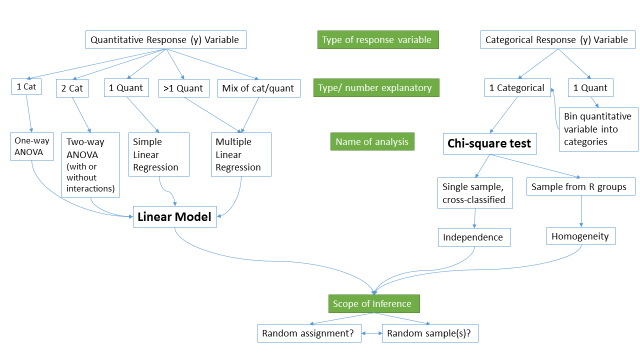
\includegraphics[width=8.89in]{chapter0_files/image001} \caption{Flow chart of methods}\label{fig:Figure1}
\end{figure}

We will be spending most of the semester working on methods for
quantitative response variables (the left side of Figure
\ref{fig:Figure1} covered in Chapters 1, 2, 3, 5, 6, and 7) and stepping
over to handle the situation with a categorical response variable (right
side of Figure \ref{fig:Figure1} that is discussed in Chapter 4).
Chapter 8 contains case studies illustrating all the methods discussed
previously, providing a final opportunity to explore additional examples
that illustrate how finding your way through the paths in Figure
\ref{fig:Figure1} leads to the appropriate analysis.

The first topics (Chapters 0 and 1) will be more familiar as we start
with single and two group situations with a quantitative response. In
your previous statistics course, you should have seen methods for
estimating and quantifying uncertainty for the mean of a single group
and for differences in the means of two groups. Once we have briefly
reviewed these methods and introduced the statistical software that we
will use throughout the course, we will consider the first new
statistical material in Chapter 2. It involves the situation with a
quantitative response variable where there are more than 2 groups to
compare -- this is what we call the \textbf{\emph{One-Way ANOVA}}
situation. It generalizes the 2-independent sample hypothesis test to
handle situations where more than 2 groups are being studied. When we
learn this method, we will begin discussing model assumptions and
methods for assessing those assumptions that will be present in every
analysis involving a quantitative response. The \textbf{\emph{Two-Way
ANOVA}} (Chapter 3) considers situations with two categorical
explanatory variables and a quantitative response. To make this somewhat
concrete, suppose we are interested in assessing differences in, say,
the \emph{yield} of wheat from a field based on the amount of
\emph{fertilizer} applied(none, low, or high) and \emph{variety} of
wheat (two types). Here, \emph{yield} is a quantitative response
variable that might be measured in bushels per acre and there are two
categorical explanatory variables, \emph{fertilizer}, with 3 levels, and
\emph{variety}, with two levels. In this material, we introduce the idea
of an \textbf{\emph{interaction}} between the two explanatory variables:
the relationship between one categorical variable and the mean of the
response changes depending on the levels of the other categorical
variable. For example, extra fertilizer might enhance the growth of one
variety and hinder the growth of another so we would say that
\emph{fertilizer} has different impacts based this interaction may or
may not actually be present, we will consider two versions of the model
in Two-Way ANOVAs, what are called the \textbf{\emph{additive}} (no
interaction) and the \textbf{\emph{interaction}} models.

Following the methods for two categorical variables and a quantitative
response, we explore a method for analyzing data where the response is
categorical, called the \textbf{\emph{Chi-square test}} in Chapter 4.
This most closely matches the One-Way ANOVA situation with a single
categorical explanatory variable, except now the response variable is
categorical. For example, we will assess whether taking a drug (vs
taking a \textbf{\emph{placebo}}\footnote{A \textbf{\emph{placebo}} is a
  treatment level designed to mimic the potentially efficacious level(s)
  but that can have no actual effect. The \textbf{\emph{placebo effect}}
  is the effect that thinking that an effective treatment was received
  has on subjects. There are other related issues in performing
  experiments like the \textbf{\emph{Hawthorne}} or observer
  \textbf{\emph{effect}} where subjects modify behavior because they are
  being observed.}) has an \textbf{\emph{effect}}\footnote{We will
  reserve the term ``effect'' for situations where we could potentially
  infer causal impacts on the response of the explanatory variable which
  occurs in situations where the levels of the explanatory variable are
  randomly assigned to the subjects.} on the type of improvement the
subjects demonstrate. There are two different scenarios for study design
that impact the analysis technique and hypotheses tested in Chapter 4.
If the explanatory variable reflects the group that subjects were
obtained from, either through randomization of the treatment level to
the subjects or by taking samples from separate populations, this is
called a \textbf{\emph{Chi-square Homogeneity Test}}. It is also
possible to obtain a single sample from a population and then obtain
information on the levels of the explanatory variable for each subject.
We will analyze these results using what is called a
\textbf{\emph{Chi-square Independence Test}}. They both use the same
test statistic but we use slightly different graphics and are testing
different hypotheses in these two related situations. Figure
\ref{fig:Figure1} also shows that if we had a quantitative explanatory
variable and a categorical response that we would need to ``bin'' or
create categories of responses from the quantitative variable to use the
Chi-square testing methods.

If the predictor and response variables are both quantitative, we start
with scatterplots, correlation, and \textbf{\emph{simple linear
regression}} models (Chapters 5 and 6) -- things you should have seen,
at least to some degree, previously. The biggest differences here will
be the depth of exploration of diagnostics and inferences for this model
and discussions of transformations of variables. If there is more than
one explanatory variable, then we say that we are doing
\textbf{\emph{multiple linear regression}} (Chapter 7) -- the
``multiple'' part of the name reflects that there will be more than one
explanatory variable. We use the same name if we have a mix of
categorical and quantitative predictor variables but there are some new
issues in setting up the models and interpreting the coefficients that
we need to consider. In the situation with one categorical predictor and
one quantitative predictor, we revisit the idea of an interaction. It
allows us to consider situations where the estimated relationship
between a quantitative predictor and the mean response varies among
different levels of the categorical variable.

By the end of Chapter 8 you should be able to identify, perform using
the statistical software R (R Core Team, 2016), and interpret the
results from each of these methods. There is a lot to learn, but many of
the tools for using R and interpreting results of the analyses
accumulate and repeat during the semester. If you work hard to
understand the initial methods, it will help you when the methods get
more complicated. You will likely feel like you are just starting to
learn how to use R at the end of the semester and for learning a new
language that is actually an accomplishment. We will just be taking you
on the first steps of a potentially long journey and it is up to you to
decide how much further you want to go with learning the software.

All the methods you will learn require you to carefully consider how the
data were collected, how that pertains to the population of interest,
and how that impacts the inferences that can be made. The
\textbf{\emph{scope of inference}} from the bottom of Figure
\ref{fig:Figure1} is our shorthand term for remembering to think about
two aspects of the study -- \textbf{\emph{random assignment}} and
\textbf{\emph{random sampling}} . In a given situation, you need to use
the description of the study to decide if the explanatory variable was
randomly assigned to study units (this allows for \textbf{\emph{causal
inferences}} if differences are detected) or not (so no causal
statements are possible). As an example, think about two studies, one
where students are randomly assigned to either get tutoring with their
statistics course or not and another where the students are asked at the
end of the semester whether they sought out tutoring or not. Suppose we
compare the final grades in the course for the two groups (tutoring/not)
and find a big difference. In the first study with random assignment, we
can say the tutoring caused the differences we observed. In the second,
we could only say that the tutoring was associated with differences but
because students self-selected the group they ended up in, we can't say
that the tutoring caused the differences. The other aspect of scope of
inference concerns random sampling: If the data were obtained using a
random sampling mechanism, then our inferences can be safely extended to
the population that the sample was taken from. However, if we have
non-random sample, our inference can only apply to the sample collected.
In the previous example, the difference would be studying a random
sample of students from the population of, say, Introductory Statistics
students at a university vs studying a sample of students that
volunteered for the research project, maybe for extra credit in the
class. We could still randomly assign them to tutoring/not but the
non-random sample would only lead to conclusions about those students
that volunteered. The most powerful scope of inference is when there are
randomly assigned levels of explanatory variables with a random sample
from population -- conclusions would be about causal impacts that would
happen in the population.

By the end of this material, you should have some basic R skills and
abilities to create basic ANOVA and Regression models, as well as to
handle Chi-squared testing situations. Together, this should prepare you
for future statistics courses or for other situations where you are
expected to be able to identify an appropriate analysis, do the
calculations for a given data set, and then effectively communicate
interpretations for the methods discussed here.

\section{Getting started in R}\label{getting-started-in-r}

You will need to download the statistical software package called R and
an enhanced interface to R called RStudio (RStudio, 2016). They are open
source and free to download and use (and will always be that way). This
means that the skills you learn now can follow you the rest of your
life. R is becoming the primary language of statistics and is being
adopted across academia, government, and businesses to help manage and
learn from the growing volume of data being obtained. Hopefully you will
get a sense of some of the power of R in this book.

The next pages will walk you through the process of getting the software
downloaded and provide you with an initial experience using RStudio to
do things that should look familiar even though the interface will be a
new experience. Do not expect to master R quickly -- it takes years
(sorry!) even if you know the statistical methods being used. We will
try to keep all your interactions with R code in a similar code format
and that should help you in learning how to use R as we move through
various methods. We will also usually provide you with example code.
Everyone that learns R starts with copying other people's code and then
making changes for specific applications -- so expect to go back to
examples from the text and focus on learning how to modify that code to
work for your particular data set. Only really experienced R users
``know'' functions without having to check other resources. After we
complete this basic introduction, Chapter 1 begins doing more
sophisticated things with R, allowing us to compare quantitative
responses from two groups, make some graphical displays, do hypothesis
testing and create confidence intervals in a couple of different ways.

You will have two downloading activities to complete before you can do
anything more than read this book\footnote{I recorded a video that walks
  through the material on the following pages that is available here:
  \url{https://camtasia.msu.montana.edu/Relay/Files/w76c139/RandRstudio_Final/RandRstudio_Final_-_20160715_130555_23.html}
  in the digital version of the book.}. First, you need to download R.
It is the engine that will do all the computing for us, but you will
only interact with it once. Go to \url{http://cran.rstudio.com} and
click on the ``\textbf{Download R for\ldots{}}'' button that corresponds
to your operating system. On the next page, click on ``\textbf{base}''
and then it will take you to a screen to download the most current
version of R that is compiled for your operating system, something like
``\textbf{Download R 3.3.1 for Windows}''. Click on that link and then
open the file you downloaded. You will need to select your preferred
language (choose English so your instructor can help you), then hit
``\textbf{Next}'' until it starts to unpack and install the program (all
the base settings will be fine). After you hit ``\textbf{Finish}'' you
will not do anything further with R directly.

Second, you need to download RStudio. It is an enhanced interface that
will make interacting with R less frustrating. To download RStudio, go
to \url{http://www.rstudio.com/products/rstudio/download/} and select
the correct version under ``Installers for Supported Platforms'' for
your operating system. Download and then install RStudio using the
installer. From this point forward, you should only open RStudio; it
provides your interface with R. Note that both R and RStudio are updated
frequently (up to four times a year) and if you downloaded either more
than a few months previously, you should download the up-to-date
versions, especially if something you are trying to do is not working.
Sometimes code will not work in older versions of R and sometimes old
code won't work in new versions of R.\footnote{The need to keep the code
  up-to-date as R continues to evolve is one reason that this book is
  locally published and that this is the 3\(^{rd}\) version in three
  years\ldots{}}

To get started, we can complete some basic tasks in R using the RStudio
interface. When you open RStudio, you will see a screen like Figure 2.
The added annotation in this and the following screen-grabs is there to
help you get initially oriented to the software interface. R is
command-line software -- meaning that most of the time you have to
create code and then enter and execute it at a command prompt to get any
results. RStudio makes the management and execution of that code more
efficient than the basic version of R. In RStudio, the lower left panel
is called the ``console'' window and is where you can type R code
directly into R or where you will see the code you run and (most
importantly!) where the results of your executed commands will show up.
The most basic interaction with R is available once you get the cursor
active at the command prompt ``\textgreater{}'' by clicking in that
panel (look for a blinking vertical line). The upper left panel is for
writing, saving, and running your R code. Once you have code available
in this window, the ``Run'' button will execute the code for the line
that your cursor is on or for any text that you have highlighted with
your mouse. The ``data management'' or environment panel is in the upper
right, providing information on what data sets have been loaded. It also
contains the ``Import Dataset'' button that provides the easiest way for
you to read a data set into R so you can analyze it. The lower right
panel contains information on the ``Packages'' (additional code we will
download and install to add functionality to R) that are available and
is where you will see plots that you make and requests for ``Help'' on
specific functions.



\begin{figure}
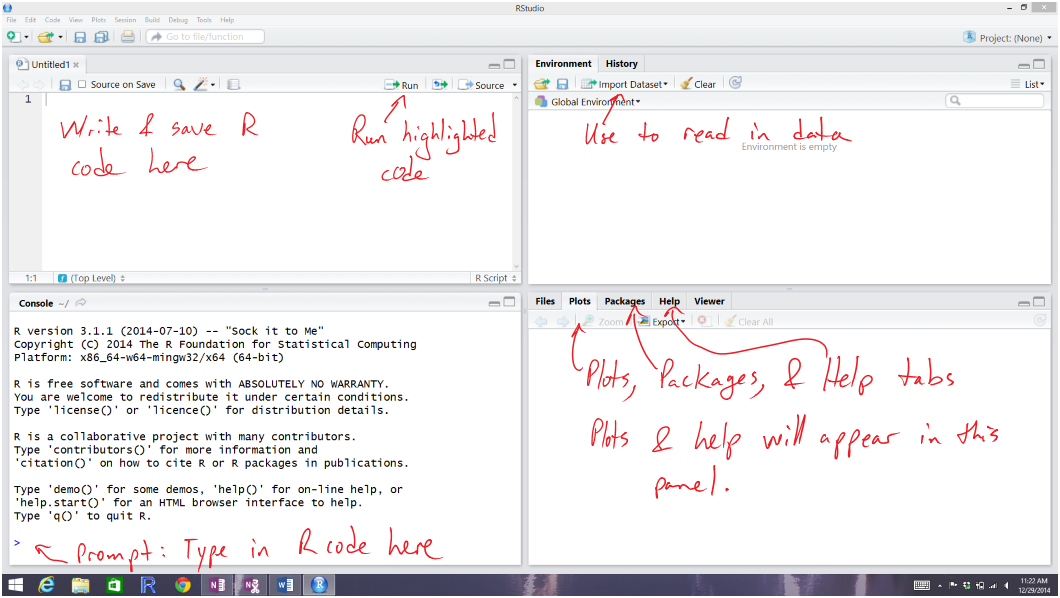
\includegraphics[width=14.72in]{chapter0_files/image003} \caption{Initial RStudio layout}\label{fig:Figure2}
\end{figure}

As a first interaction with R we can use it as a calculator. To do this,
click near the command prompt (\texttt{\textgreater{}}) in the lower
left ``console'' panel, type 3+4, and then hit enter. It should look
like this:

\begin{Shaded}
\begin{Highlighting}[]
\NormalTok{>}\StringTok{ }\DecValTok{3+4}
\NormalTok{[}\DecValTok{1}\NormalTok{] }\DecValTok{7}
\end{Highlighting}
\end{Shaded}

You can do more interesting calculations, like finding the mean of the
numbers 3, 5, 7, and 8 by adding them up and dividing by 4:

\begin{Shaded}
\begin{Highlighting}[]
\NormalTok{>}\StringTok{ }\NormalTok{(-}\DecValTok{3+5+7+8}\NormalTok{)/}\DecValTok{4}
\NormalTok{[}\DecValTok{1}\NormalTok{] }\DecValTok{4}\NormalTok{. }\DecValTok{25}
\end{Highlighting}
\end{Shaded}

Note that the parentheses help R to figure out your desired order of
operations. If you drop that grouping, you get a very different (and
wrong!) result:

\begin{Shaded}
\begin{Highlighting}[]
\NormalTok{>}\StringTok{ }\NormalTok{-}\DecValTok{3+5+7+8}\NormalTok{/}\DecValTok{4}
\NormalTok{[}\DecValTok{1}\NormalTok{] }\DecValTok{11}
\end{Highlighting}
\end{Shaded}

We could estimate the standard deviation similarly using the formula you
might remember from introductory statistics, but that will only work in
very limited situations. To use the real power of R this semester, we
need to work with data sets that store the Basically, we need to store
observations in named vectors (one dimensional arrays) that contain a
list of the observations. To create a vector containing the four numbers
and assign it to a variable named \emph{variable1}, we need to create a
vector using the function \texttt{c} which means ``combine the items''
that follow, if they are inside parentheses and have commas separating
the values, as follows:

\begin{Shaded}
\begin{Highlighting}[]
\NormalTok{>}\StringTok{ }\KeywordTok{c}\NormalTok{(-}\DecValTok{3}\NormalTok{, }\DecValTok{5}\NormalTok{, }\DecValTok{7}\NormalTok{, }\DecValTok{8}\NormalTok{)}
\NormalTok{[}\DecValTok{1}\NormalTok{] -}\DecValTok{3} \DecValTok{5} \DecValTok{7} \DecValTok{8}
\end{Highlighting}
\end{Shaded}

To get this vector stored in a variable called \emph{variable1} we need
to use the assignment operator, \texttt{\textless{}-} (read as ``stored
as'') that assigns the information on the right into the variable that
you are creating on the left.

\begin{Shaded}
\begin{Highlighting}[]
\NormalTok{>}\StringTok{ }\NormalTok{variable1 <-}\StringTok{ }\KeywordTok{c}\NormalTok{(-}\DecValTok{3}\NormalTok{, }\DecValTok{5}\NormalTok{, }\DecValTok{7}\NormalTok{, }\DecValTok{8}\NormalTok{)}
\end{Highlighting}
\end{Shaded}

In R, the assignment operator, \texttt{\textless{}-}, is created by
typing a ``less than'' symbol \texttt{\textless{}} followed by a
``minus'' sign (\texttt{-}) ever want to see what numbers are residing
in an object in R, just type its name and hit \emph{enter}. You can see
how that variable contains the same information that was initially
generated by \texttt{c(-3,\ 5,\ 7,\ 8)} but is easier to access since we
just need the text for the variable name representing that vector.

\begin{Shaded}
\begin{Highlighting}[]
\NormalTok{>}\StringTok{ }\NormalTok{variable1}
\NormalTok{[}\DecValTok{1}\NormalTok{] -}\DecValTok{3} \DecValTok{5} \DecValTok{7} \DecValTok{8}
\end{Highlighting}
\end{Shaded}

With the data stored in a variable, wean use functions such as
\texttt{mean} and \texttt{sd} to find the mean and standard deviation of
the observations contained in \texttt{variable1} :

\begin{Shaded}
\begin{Highlighting}[]
\NormalTok{>}\StringTok{ }\KeywordTok{mean}\NormalTok{(variable1)}
\NormalTok{[}\DecValTok{1}\NormalTok{] }\FloatTok{4.25}
\NormalTok{>}\StringTok{ }\KeywordTok{sd}\NormalTok{(variable1)}
\NormalTok{[}\DecValTok{1}\NormalTok{] }\FloatTok{4.99166}
\end{Highlighting}
\end{Shaded}

When dealing with real data, we will often have information about more
than one variable. We could enter all observations by hand for each
variable but this is prone to error and onerous for all but the smallest
data sets. If you are to ever utilize the power of statistics in the
evolving data-centered world, data management has to be accomplished in
a more sophisticated way. While you can manage data sets quite
effectively in R, it is often easiest to start with your data set in
something like Microsoft Excel or OpenOffice's Calc. You want to make
sure that observations are in the rows and the names of variables are in
the columns and that there is no ``extra stuff'' in the spreadsheet. If
you have missing observations, they should be represented with blank
cells. The file should be saved as a ``.csv'' file (stands for
comma-separated values although Excel calls it ``CSV (Comma
Delimited)'', which basically strips off some of the junk that Excel
adds to the necessary information in the file. Excel will tell you that
this is a bad idea, but it actually creates a more stable archival
format and one that R can use directly\footnote{There are ways to read
  ``.xls'' and ``.xlsx'' files directly into R but to handle multiple
  sheets they are more complicated and not as stable across operating
  systems as the simpler version we recommend.}.

With data set converted to a CSV file, we need to read the data set into
R. There are two ways to do this, either using the point-and-click GUI
in RStudio (click the ``Import Data Set'' button in the upper right
``Environment'' panel as indicated in Figure \ref{fig:Figure2}) or
modifying the

\texttt{read.csv} function to find the file of interest. To practice
this, you can download an Excel (.xls) file from
\url{http://www.math.montana.edu/courses/s217/documents/treadmill.xls}
31 males that volunteered for a study on methods for measuring
fitness(Westfall and Young, 1993). In the spreadsheet, you will find a
data set that starts and ends with the following information (only
results for Subjects 1, 2, 30, and 31 shown here):

\begin{longtable}[]{@{}lllrrlrr@{}}
\toprule
\begin{minipage}[b]{0.07\columnwidth}\raggedright\strut
Sub- ject\strut
\end{minipage} & \begin{minipage}[b]{0.10\columnwidth}\raggedright\strut
Tread- MillOx\strut
\end{minipage} & \begin{minipage}[b]{0.14\columnwidth}\raggedright\strut
TreadMill- MaxPulse\strut
\end{minipage} & \begin{minipage}[b]{0.09\columnwidth}\raggedleft\strut
RunTime\strut
\end{minipage} & \begin{minipage}[b]{0.10\columnwidth}\raggedleft\strut
RunPulse\strut
\end{minipage} & \begin{minipage}[b]{0.08\columnwidth}\raggedright\strut
Rest Pulse\strut
\end{minipage} & \begin{minipage}[b]{0.15\columnwidth}\raggedleft\strut
BodyWeight\strut
\end{minipage} & \begin{minipage}[b]{0.04\columnwidth}\raggedleft\strut
Age\strut
\end{minipage}\tabularnewline
\midrule
\endhead
\begin{minipage}[t]{0.07\columnwidth}\raggedright\strut
1\strut
\end{minipage} & \begin{minipage}[t]{0.10\columnwidth}\raggedright\strut
60.05\strut
\end{minipage} & \begin{minipage}[t]{0.14\columnwidth}\raggedright\strut
186\strut
\end{minipage} & \begin{minipage}[t]{0.09\columnwidth}\raggedleft\strut
8.63\strut
\end{minipage} & \begin{minipage}[t]{0.10\columnwidth}\raggedleft\strut
170\strut
\end{minipage} & \begin{minipage}[t]{0.08\columnwidth}\raggedright\strut
48\strut
\end{minipage} & \begin{minipage}[t]{0.15\columnwidth}\raggedleft\strut
81.87\strut
\end{minipage} & \begin{minipage}[t]{0.04\columnwidth}\raggedleft\strut
38\strut
\end{minipage}\tabularnewline
\begin{minipage}[t]{0.07\columnwidth}\raggedright\strut
2\strut
\end{minipage} & \begin{minipage}[t]{0.10\columnwidth}\raggedright\strut
59.57\strut
\end{minipage} & \begin{minipage}[t]{0.14\columnwidth}\raggedright\strut
172\strut
\end{minipage} & \begin{minipage}[t]{0.09\columnwidth}\raggedleft\strut
8.17\strut
\end{minipage} & \begin{minipage}[t]{0.10\columnwidth}\raggedleft\strut
166\strut
\end{minipage} & \begin{minipage}[t]{0.08\columnwidth}\raggedright\strut
40\strut
\end{minipage} & \begin{minipage}[t]{0.15\columnwidth}\raggedleft\strut
68.15\strut
\end{minipage} & \begin{minipage}[t]{0.04\columnwidth}\raggedleft\strut
42\strut
\end{minipage}\tabularnewline
\begin{minipage}[t]{0.07\columnwidth}\raggedright\strut
\ldots{}\strut
\end{minipage} & \begin{minipage}[t]{0.10\columnwidth}\raggedright\strut
\ldots{}\strut
\end{minipage} & \begin{minipage}[t]{0.14\columnwidth}\raggedright\strut
\ldots{}\strut
\end{minipage} & \begin{minipage}[t]{0.09\columnwidth}\raggedleft\strut
\ldots{}\strut
\end{minipage} & \begin{minipage}[t]{0.10\columnwidth}\raggedleft\strut
\ldots{}\strut
\end{minipage} & \begin{minipage}[t]{0.08\columnwidth}\raggedright\strut
\ldots{}\strut
\end{minipage} & \begin{minipage}[t]{0.15\columnwidth}\raggedleft\strut
\ldots{}\strut
\end{minipage} & \begin{minipage}[t]{0.04\columnwidth}\raggedleft\strut
\ldots{}\strut
\end{minipage}\tabularnewline
\begin{minipage}[t]{0.07\columnwidth}\raggedright\strut
30\strut
\end{minipage} & \begin{minipage}[t]{0.10\columnwidth}\raggedright\strut
39.2\strut
\end{minipage} & \begin{minipage}[t]{0.14\columnwidth}\raggedright\strut
172\strut
\end{minipage} & \begin{minipage}[t]{0.09\columnwidth}\raggedleft\strut
12.88\strut
\end{minipage} & \begin{minipage}[t]{0.10\columnwidth}\raggedleft\strut
168\strut
\end{minipage} & \begin{minipage}[t]{0.08\columnwidth}\raggedright\strut
44\strut
\end{minipage} & \begin{minipage}[t]{0.15\columnwidth}\raggedleft\strut
91.63\strut
\end{minipage} & \begin{minipage}[t]{0.04\columnwidth}\raggedleft\strut
54\strut
\end{minipage}\tabularnewline
\begin{minipage}[t]{0.07\columnwidth}\raggedright\strut
31\strut
\end{minipage} & \begin{minipage}[t]{0.10\columnwidth}\raggedright\strut
37.39\strut
\end{minipage} & \begin{minipage}[t]{0.14\columnwidth}\raggedright\strut
192\strut
\end{minipage} & \begin{minipage}[t]{0.09\columnwidth}\raggedleft\strut
14.03\strut
\end{minipage} & \begin{minipage}[t]{0.10\columnwidth}\raggedleft\strut
186\strut
\end{minipage} & \begin{minipage}[t]{0.08\columnwidth}\raggedright\strut
56\strut
\end{minipage} & \begin{minipage}[t]{0.15\columnwidth}\raggedleft\strut
87.66\strut
\end{minipage} & \begin{minipage}[t]{0.04\columnwidth}\raggedleft\strut
45\strut
\end{minipage}\tabularnewline
\bottomrule
\end{longtable}

The variables contain information on the subject number
(\emph{Subject}), subjects' treadmill oxygen consumption
(\emph{TreadMillOx}, in ml per kg per minute) and maximum pulse rate
(\emph{TreadMillMaxPulse}, in beats per minute), time to run 1.5 miles
(\emph{Run Time}, in minutes), maximum pulse during 1.5 mile run
(\emph{RunPulse}, in beats per minute), resting pulse rate
(\emph{RestPulse}, beats per minute), Body Weight (\emph{BodyWeight}, in
kg), and \emph{Age} (in years). Open the file in Excel or equivalent
software and then save it as a .csv file in a location you can find on
your computer. Then go to RStudio and click on \textbf{File} , then
\textbf{Import Dataset} , then \textbf{From CSV\ldots{}}\footnote{If you
  are having trouble getting the file converted and read into R, copy
  and run the following code:
  \texttt{treadmill\ \textless{}-read.csv("http://www.math.montana.edu/courses/s217/documents/treadmill.csv",\ header=T)}.}
Find your file and check ``\textbf{Import}''. R will store the data set
as an object named whatever the .csv file was named. You could use
another name as well, but it is often easiest just to keep the data set
name in R related to the original file name. You should see some text
appear in the console (lower left panel) like in Figure
\ref{fig:Figure3}. The text that is created will look something like the
following -- if you had stored the file in a drive labeled D:, it would
be:

\begin{Shaded}
\begin{Highlighting}[]
\NormalTok{treadmill <-}\StringTok{ }\KeywordTok{read.csv}\NormalTok{(}\StringTok{"D:/treadmill.csv"}\NormalTok{)}
\end{Highlighting}
\end{Shaded}

What is put inside the \texttt{"\ "} will depend on the location and
name of your saved .csv file. A version of the data set in what looks
like a spreadsheet will appear in the upper left window due to the
second line of code (\texttt{View(treadmill})).



\begin{figure}
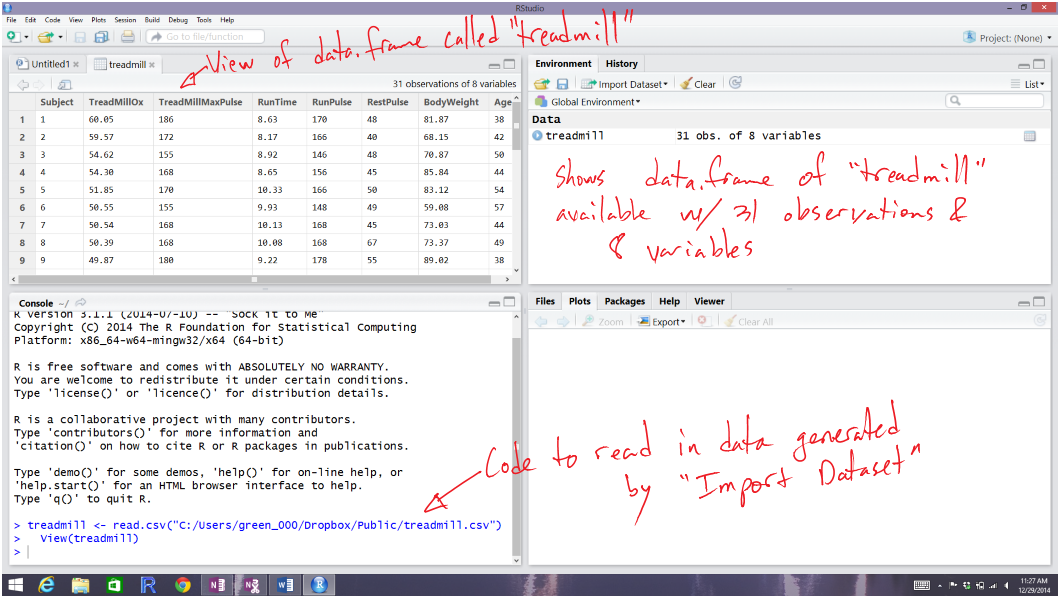
\includegraphics[width=14.72in]{chapter0_files/image005} \caption{RStudio with initial data set loaded}\label{fig:Figure3}
\end{figure}

Just directly typing (or using) a line of code like this is actually the
other way that we can read in files. If you choose to use the text-only
interface, then you need to tell R where to look in your computer to
find the data file. \texttt{read.csv} is a function that takes a path as
an argument. To use it, specify the path to your data file, put quotes
around it, and put it as the input to \texttt{read.csv(...)} . For some
examples later in the book, you will be able to copy a command like this
from the text and read data sets and other code directly from my the
course folder, assuming you are connected to the internet.

To verify that you read the data set in correctly, it is always good to
check its contents. We can view the first and last rows in the data set
using the \texttt{head} and \texttt{tail} functions on the data set,
which show the following results for the \texttt{treadmill} data. Note
that you will sometimes need to resize the console window in RStudio to
get all the columns to display in a single row which can be performed by
dragging the gray bars that separate the panels.

\begin{Shaded}
\begin{Highlighting}[]
\KeywordTok{head}\NormalTok{(treadmill)}
\end{Highlighting}
\end{Shaded}

\begin{verbatim}
##   Subject TreadMillOx TreadMillMaxPulse RunTime RunPulse RestPulse
## 1       1       60.05               186    8.63      170        48
## 2       2       59.57               172    8.17      166        40
## 3       3       54.62               155    8.92      146        48
## 4       4       54.30               168    8.65      156        45
## 5       5       51.85               170   10.33      166        50
## 6       6       50.55               155    9.93      148        49
##   BodyWeight Age
## 1      81.87  38
## 2      68.15  42
## 3      70.87  50
## 4      85.84  44
## 5      83.12  54
## 6      59.08  57
\end{verbatim}

\begin{Shaded}
\begin{Highlighting}[]
\KeywordTok{tail}\NormalTok{(treadmill)}
\end{Highlighting}
\end{Shaded}

\begin{verbatim}
##    Subject TreadMillOx TreadMillMaxPulse RunTime RunPulse RestPulse
## 26      26       44.61               182   11.37      178        62
## 27      27       40.84               172   10.95      168        57
## 28      28       39.44               176   13.08      174        63
## 29      29       39.41               176   12.63      174        58
## 30      30       39.20               172   12.88      168        44
## 31      31       37.39               192   14.03      186        56
##    BodyWeight Age
## 26      89.47  44
## 27      69.63  51
## 28      81.42  44
## 29      73.37  57
## 30      91.63  54
## 31      87.66  45
\end{verbatim}

While not always required, for many of the analyses, we will tap into a
large suite of additional functions available in R packages by
``installing'' (basically downloading) and then ``loading'' the
packages. There are some packages that we will use frequently, starting
with the \texttt{mosaic} package (Pruim, Kaplan, and Horton, tab in the
lower right panel of RStudio. Click on the \textbf{Install} button and
then type in the name of the package in the box (here type in
\texttt{mosaic}). RStudio will try to auto-complete the package name you
are typing which should help you make sure you got it typed correctly.
This will be the first of \emph{many} times that we will mention that R
is case sensitive -- in other words, \texttt{Mosaic} is different from
\texttt{mosaic} in R syntax and this sort of thing applies to everything
you do in R. You should only need to install each R package once on a
given computer. If you ever see a message that R can't find a package,
make sure it appears in the list in the \textbf{Packages} tab and if it
doesn't, repeat the previous steps to install it.

After installing the package, we need to load it to make it active in a
given work session. Go to the command prompt and type (or copy and
paste) \texttt{require(mosaic)} :

\begin{Shaded}
\begin{Highlighting}[]
\KeywordTok{require}\NormalTok{(mosaic)}
\end{Highlighting}
\end{Shaded}

You may see a warning message about versions of the package and versions
of R -- this is \emph{usually} something you can ignore. Other warning
messages could be more ominous for proceeding but before getting too
concerned, there are couple of basic things to check. First, double
check that the package is installed (see previous steps). Second, check
for typographical errors in your code -- especially for mis-spellings or
unintended capitalization. If you are still having issues, try repeating
the installation process. If that fails, find someone more used to using
R to help you (for example in the Math Learning Center or by emailing
your instructor)\footnote{Most computer lab computers at Montana State
  University have RStudio installed and so provide another venue to try
  this where the software is already installed.}.

To help you go from basic to intermediate R usage and especially to help
with more complicated problems, you will want to learn how to manage and
save your R code. The best way to do this is using the upper left panel
in RStudio using what are called R Scripts, which are files that have a
file extension of ``.R''. To start a new ``.R''" file to store your
code, click on \textbf{File} , then \textbf{New File}, then **R Script*.
This will create a blank page to enter and edit code -- then save the
file as MyFileName.R in your preferred location. Saving your code will
mean that you can return to where you last were working by simply
re-running the saved script file. With code in the script window, you
can place the cursor on a line of code or highlight a chunk of code and
hit the ``Run'' button on the upper part of the panel. It will appear in
the console with results just like what you would obtain if you typed it
after the command prompt and hit enter for each line.

Figure \ref{fig:Figure4} shows the screen with the code used in this
section in the upper left panel, saved in file called Ch0.R, with the
results of highlighting and executing the first section of code using
the ``Run'' button.



\begin{figure}
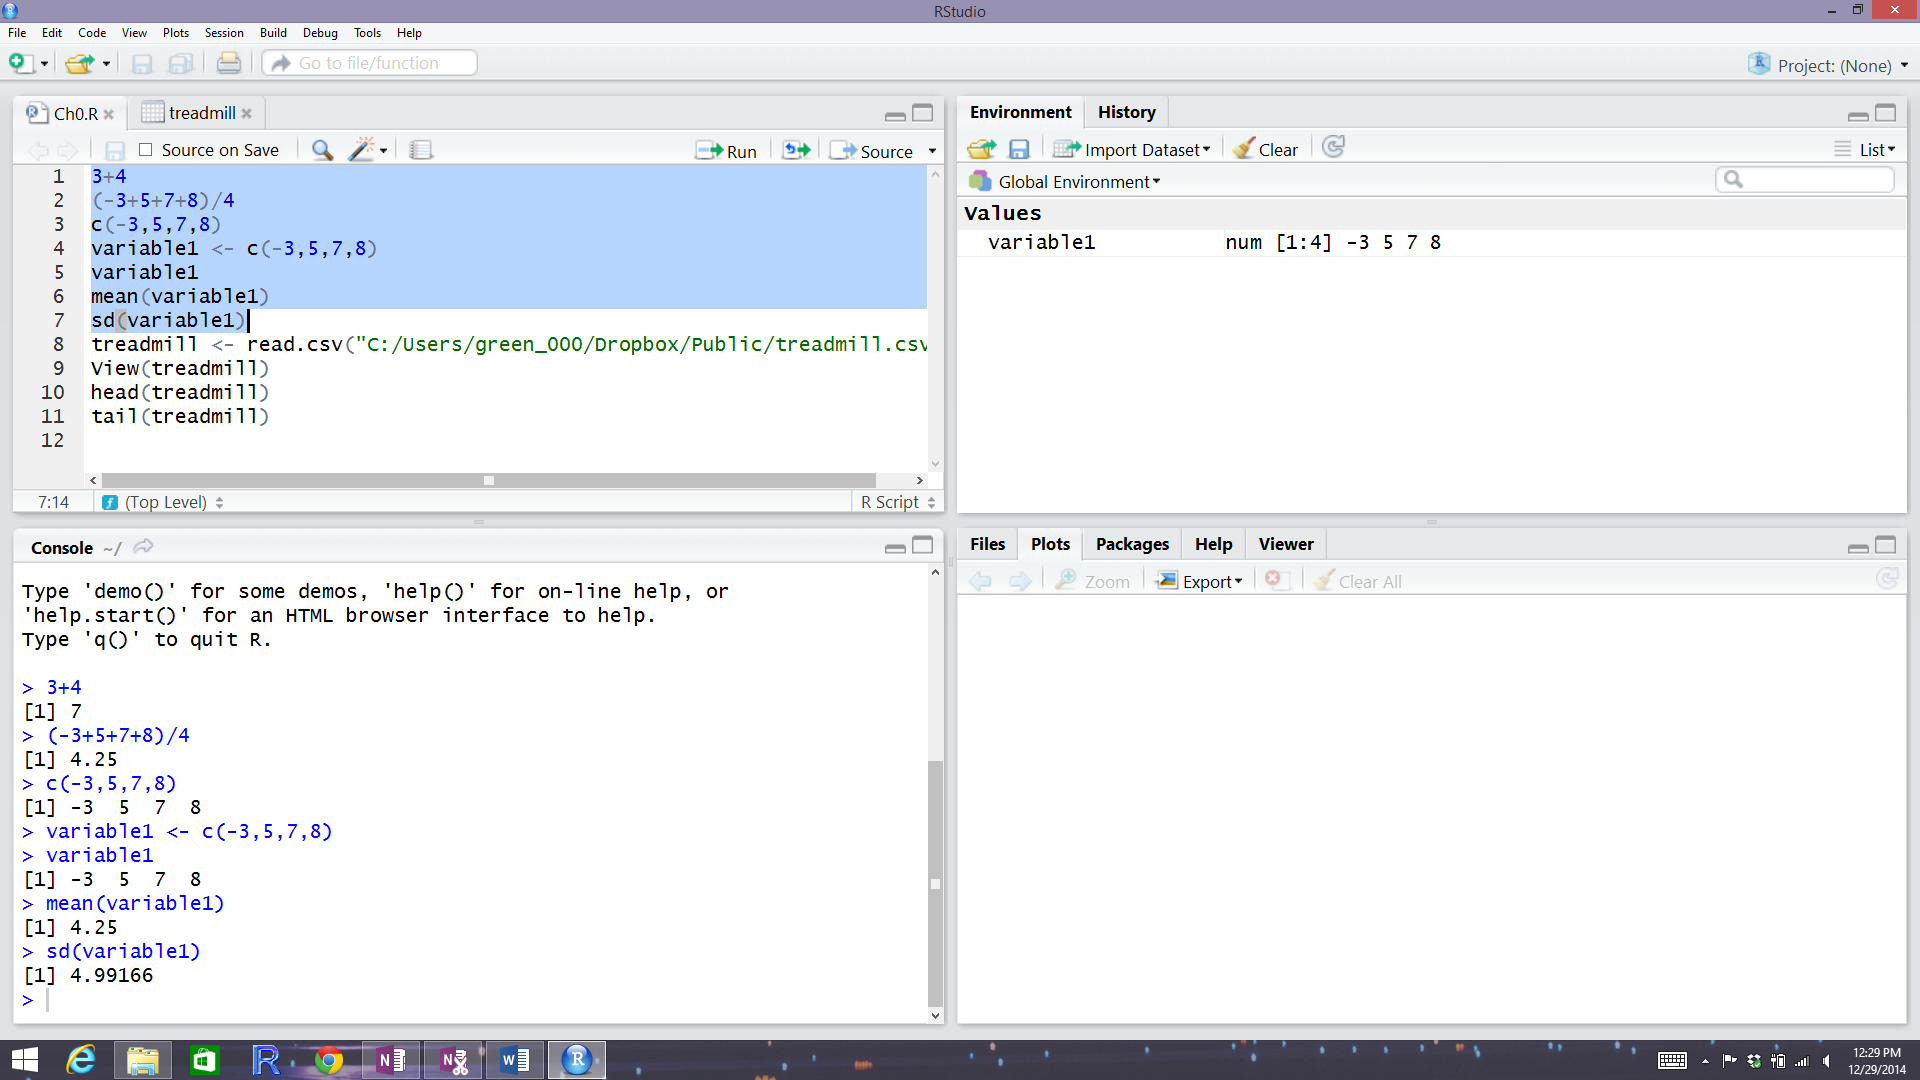
\includegraphics[width=26.67in]{chapter0_files/image006} \caption{RStudio with highlighted code run}\label{fig:Figure4}
\end{figure}

\section{Basic summary statistics, histograms, and boxplots using
R}\label{basic-summary-statistics-histograms-and-boxplots-using-r}

With RStudio running, the \texttt{mosaic} package loaded, a place to
write and save code, and the \texttt{treadmill} data set loaded, we can
(finally!) start to summarize the results of the study. The
\texttt{treadmill} object is what R calls a
\textbf{\emph{data.frame}}\footnote{Data frames in R are objects that
  can contain both categorical and quantitative variables on your n
  subjects with a name for each variable that is also the name of each
  column in a matrix. Each subject is a row of the data set.} and
contains columns corresponding to each variable in the spreadsheet.
Every function in R will involve specifying the variable(s) of interest
and how you want to use them. To access a particular variable (column)
in a data. frame, you can use a \$ between the data. frame name and the
name of the variable of interest, generically as
\texttt{dataframename\$variablename}. To identify the \texttt{RunTime}
variable here it would be \texttt{treadmill\$RunTime}. In the command
line it would look like:

\begin{Shaded}
\begin{Highlighting}[]
\NormalTok{treadmill$RunTime}
\end{Highlighting}
\end{Shaded}

\begin{verbatim}
##  [1]  8.63  8.17  8.92  8.65 10.33  9.93 10.13 10.08  9.22  8.95 10.85
## [12]  9.40 11.50 10.50 10.60 10.25 10.00 11.17 10.47 11.95  9.63 10.07
## [23] 11.08 11.63 11.12 11.37 10.95 13.08 12.63 12.88 14.03
\end{verbatim}

Just as in the previous section, we can generate summary statistics
using functions like \texttt{mean} and \texttt{sd} by running them on a
specific variable:

\begin{Shaded}
\begin{Highlighting}[]
\KeywordTok{mean}\NormalTok{(treadmill$RunTime)}
\end{Highlighting}
\end{Shaded}

\begin{verbatim}
## [1] 10.58613
\end{verbatim}

\begin{Shaded}
\begin{Highlighting}[]
\KeywordTok{sd}\NormalTok{(treadmill$RunTime)}
\end{Highlighting}
\end{Shaded}

\begin{verbatim}
## [1] 1.387414
\end{verbatim}

And now we know that the average running time for 1.5 miles for the
subjects in the study was 10.6 minutes with a standard deviation (SD) of
1.39 minutes. But you should remember that the mean and SD are only
appropriate summaries if the distribution is roughly
\textbf{\emph{symmetric}} (both sides of the distribution are
approximately the same). The \texttt{mosaic} package provides a useful
function called \texttt{favstats} that provides the mean and SD as well
as the \textbf{\emph{5 number summary}} : the minimum (\texttt{min}),
the first quartile (\texttt{Q1}, the 25\(^{th}\) percentile), the median
(50\(^{th}\) percentile), the third quartile (\texttt{Q3} , the
75\(^{th}\) percentile), and the maximum (\texttt{max}). It also
provides the number of observations (\texttt{n}) which was 31, as noted
above, and a count of whether any missing values were encountered
(\texttt{missing}), which was 0 here since all subjects had measurements
available on this variable.

\begin{Shaded}
\begin{Highlighting}[]
\KeywordTok{favstats}\NormalTok{(treadmill$RunTime)}
\end{Highlighting}
\end{Shaded}

\begin{verbatim}
##   min   Q1 median    Q3   max     mean       sd  n missing
##  8.17 9.78  10.47 11.27 14.03 10.58613 1.387414 31       0
\end{verbatim}

We are starting to get somewhere with understanding that the runners
were somewhat fit with worst runner covering 1.5 miles in 14 minutes
(the equivalent of a 9.3 minute mile) and the best running at a 5.4
minute mile pace. The limited variation in the results suggests that the
sample was obtained from a restricted group with somewhat common
characteristics. When you explore the ages and weights of the subjects
in the Practice Problems in Section 0.5, you will get even more
information about how similar all the subjects in this study were.

A graphical display of these results will help us to assess the shape of
the distribution of run times -- including considering the potential for
the presence of a \textbf{\emph{skew}} (whether the right or left tail
of the distribution is noticeably more spread out with left skew meaning
that the left tail is more spread out than the right tail) and
\textbf{\emph{outliers}}\\
(unusual observations). A \textbf{\emph{histogram }} is a good place to
start. Histograms display connected bars with counts of observations
defining the height of bars based on a set of bins of values of the
quantitative variable. We will apply the \texttt{hist} function to the
\texttt{RunTime} variable, which produces Figure \ref{fig:Figure5}.




\begin{Shaded}
\begin{Highlighting}[]
\KeywordTok{hist}\NormalTok{(treadmill$RunTime)}
\end{Highlighting}
\end{Shaded}

\begin{figure}[htbp]
\centering
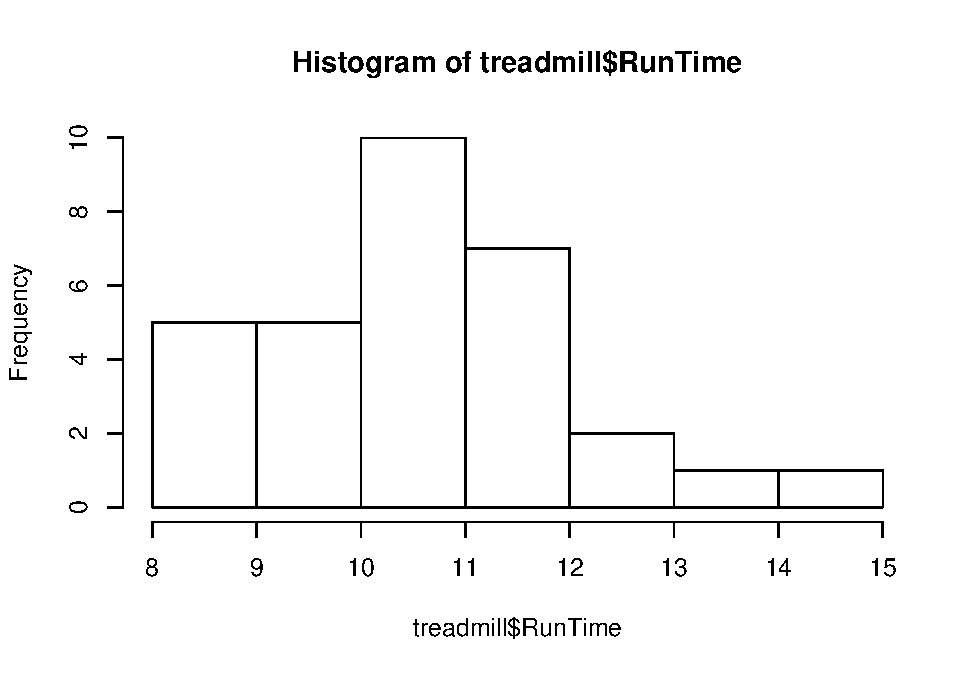
\includegraphics{GreenwoodBanner_files/figure-latex/Figure5-1.pdf}
\caption{\label{fig:Figure5}Histogram of Run Times \#(minutes) of n=31 subjects in
Treadmill study.}
\end{figure}

I used the \textbf{Export} button found above the plot, followed by
\textbf{Copy to Clipboard} and clicking on the \textbf{Copy Plot}
button. Then if you open your favorite word-processing program, you
should be able to paste it into a document for writing reports that
include the figures. You can see the first parts of this process in the
screen grab in Figure \ref{fig:Figure6}.



\begin{figure}
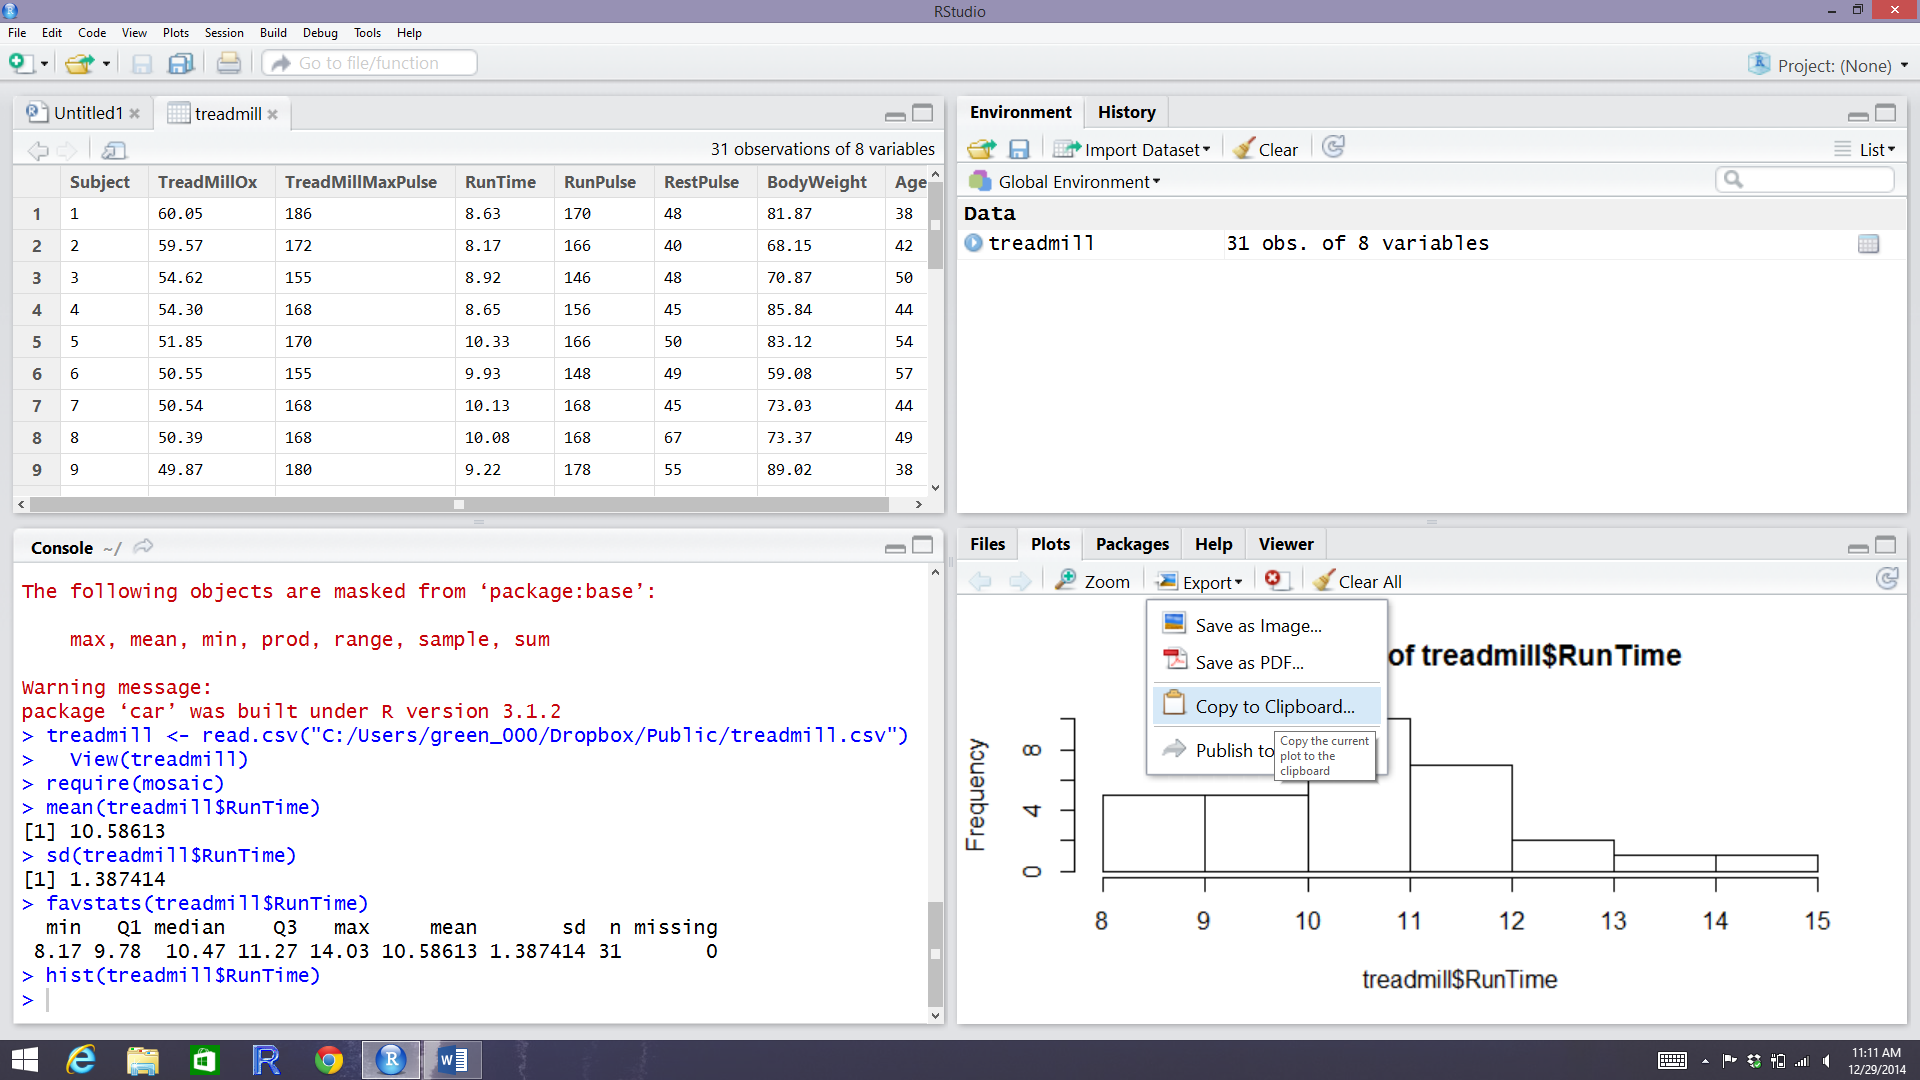
\includegraphics[width=26.67in]{chapter0_files/image010} \caption{RStudio while in the process of copying the histogram}\label{fig:Figure6}
\end{figure}

You can also directly save the figures as separate files using
\textbf{Save as Image} or \textbf{Save as PDF}and then insert them into
your word processing documents.

The function \texttt{hist} defaults into providing a histogram on the
\textbf{\emph{frequency}} (count) scale. In most R functions, there are
the default options that will occur if we don't make any specific
choices but we can override the default options if we desire. One option
we can modify here is to add labels to the bars to be able to see
exactly how many observations fell into each bar. Specifically, we can
turn the \texttt{labels} option ``on'' by making it true (``T'') by
adding \texttt{labels=T} to the previous call to the \texttt{hist}
function, separated by a comma:



\begin{Shaded}
\begin{Highlighting}[]
\KeywordTok{hist}\NormalTok{(treadmill$RunTime, }\DataTypeTok{labels=}\NormalTok{T)}
\end{Highlighting}
\end{Shaded}

\begin{figure}[htbp]
\centering
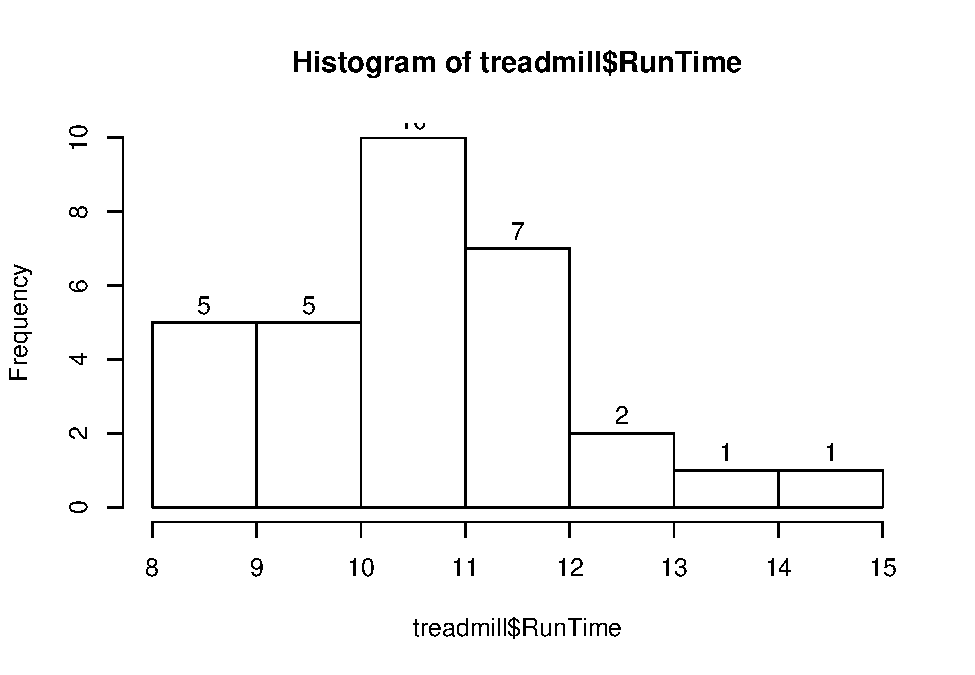
\includegraphics{GreenwoodBanner_files/figure-latex/Figure7-1.pdf}
\caption{\label{fig:Figure7}Histogram of \#Run Times with counts in bars labeled.}
\end{figure}

Based on this histogram, it does not appear that there any outliers in
the responses since there are no bars that are separated from the other
observations. However, the distribution does not look symmetric and
there might be a skew to the distribution. Specifically, it appears to
be \textbf{\emph{skewed right}} (the right tail is longer than the
left). But histograms can sometimes mask features of the data set by
binning observations and it is hard to find the percentiles accurately
from the plot.

When assessing outliers and skew, the \textbf{\emph{boxplot}}\\
(or \emph{Box and Whiskers} plot) can also be helpful (Figure
\ref{fig:Figure8}) to describe the shape of the distribution as it
displays the 5-number summary and will also indicate observations that
are ``far'' above the middle of the observations. R's \texttt{boxplot}
function uses the standard rule to indicate an observation as a
\textbf{\emph{potential outlier}} if it falls more than 1.5 times the
\textbf{\emph{IQR}} (Inter-Quartile Range, calculated as Q3-Q1) below Q1
or above Q3. The potential outliers are plotted with circles and the
\emph{Whiskers} (lines that extend from Q1 and Q3 typically to the
minimum and maximum) are shortened to only go as far as observations
that are within \(1.5*\)IQR of the upper and lower quartiles. The
\emph{box} part of the boxplot is a box that goes from Q1 to Q3 and the
median is displayed as a line somewhere inside the box\footnote{The
  median, quartiles and whiskers sometimes occur at the same values when
  there are many tied observations. If you can't see all the components
  of the boxplot, produce the numerical summary to help you understand
  what happened.}. Looking back at the summary statistics above, Q1=9.78
and Q3=11.27, providing an IQR of:

\begin{Shaded}
\begin{Highlighting}[]
\NormalTok{IQR <-}\StringTok{ }\FloatTok{11.27} \NormalTok{-}\StringTok{ }\FloatTok{9.78}
\end{Highlighting}
\end{Shaded}

One observation (the maximum value of 14.03) is indicated as a potential
outlier based on this result by being larger than Q3 \(+1.5*\)IQR, which
was 13.505:

\begin{Shaded}
\begin{Highlighting}[]
\FloatTok{11.27} \NormalTok{+}\StringTok{ }\FloatTok{1.5}\NormalTok{*IQR}
\end{Highlighting}
\end{Shaded}

\begin{verbatim}
## [1] 13.505
\end{verbatim}

The boxplot also shows a slight indication of a right skew (skew towards
larger values) with the distance from the minimum to the median being
smaller than the distance from the median to the maximum. Additionally,
the distance from Q1 to the median is smaller than the distance from the
median to Q3. It is modest skew, but worth noting.



\begin{Shaded}
\begin{Highlighting}[]
\KeywordTok{boxplot}\NormalTok{(treadmill$RunTime)}
\end{Highlighting}
\end{Shaded}

\begin{figure}[htbp]
\centering
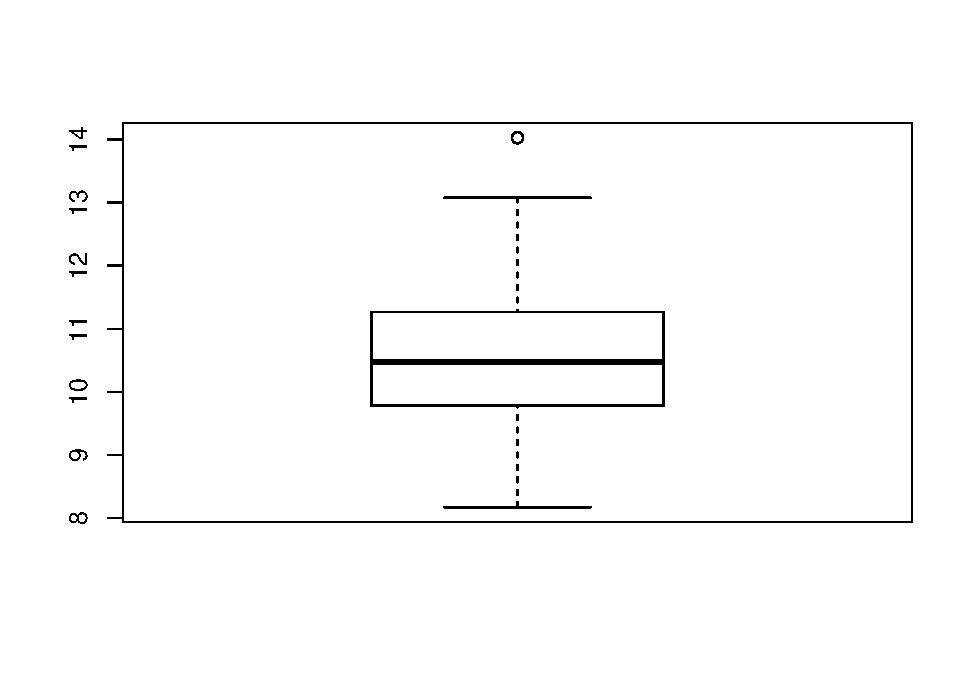
\includegraphics{GreenwoodBanner_files/figure-latex/Figure8-1.pdf}
\caption{\label{fig:Figure8}Boxplot of 1.5 mile Run Times.}
\end{figure}

While the default boxplot is fine, it fails to provide good graphical
labels, especially on the y-axis. Additionally, there is no title on the
plot. The following code provides some enhancements to the plot by using
the \texttt{ylab} and \texttt{main} options in the call to
\texttt{boxplot}, with the results displayed in Figure
\ref{fig:Figure9}. When we add text to plots, it will be contained
within quotes and be assigned into the options \texttt{ylab} (for
y-axis) or \texttt{main} (for the title) here to put it into those
locations.



\begin{Shaded}
\begin{Highlighting}[]
\KeywordTok{boxplot}\NormalTok{(treadmill$RunTime, }\DataTypeTok{ylab=}\StringTok{"1.5 Mile Run Time (minutes)"}\NormalTok{, }
        \DataTypeTok{main=}\StringTok{"Boxplot of the Run Times of n=31 participants"}\NormalTok{)}
\end{Highlighting}
\end{Shaded}

\begin{figure}[htbp]
\centering
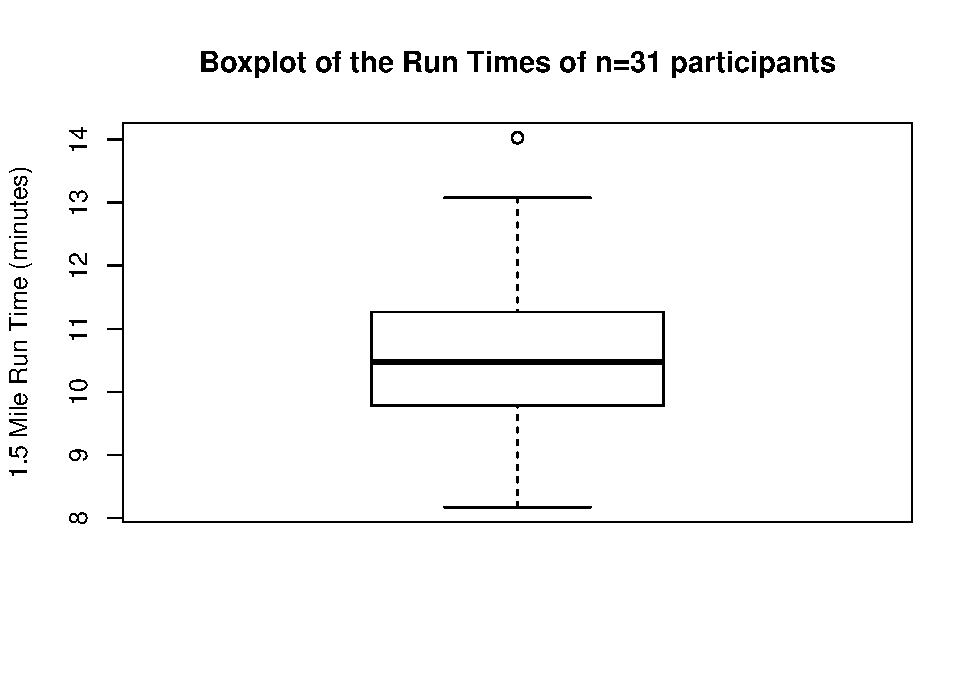
\includegraphics{GreenwoodBanner_files/figure-latex/Figure9-1.pdf}
\caption{\label{fig:Figure9}Boxplot of Run Times with improved labels.}
\end{figure}

Throughout the book, we will often use extra options to make figures
that are easier for you to understand. There are often simpler versions
of the functions that will suffice but the extra work to get better
labeled figures is often worth it. I guess the point is that ``a picture
is worth a thousand words'' but in data visualization, that is only true
if the reader can understand what is being displayed. It is also
important to think about the quality of the information that is being
displayed, regardless of how pretty the graphic might be.

All the previous results were created by running the R code and then
``grabbing'' the results from either the console or by copying the
figure. There is another way to use RStudio where you can have it
compile the results (both output and figures) directly into a document
together with the code that generated it, using what is called RMarkdown
(\url{http://shiny.rstudio.com/articles/rmarkdown.html}). It adds some
additional setup complexity we want to avoid for now but is what we used
to do all the analyses that follow in the book. The main reason to
mention this is that you will see a change in formatting of the R code
and output from here forward as you will no longer see the command
prompt (``\textgreater{}'') with the code. The output will be flagged by
having two ``\#\#'''s before it. For example, the summary statistics for
the \emph{RunTime} variable from `\texttt{favstats} function would look
like:

\begin{Shaded}
\begin{Highlighting}[]
\KeywordTok{favstats}\NormalTok{(treadmill$RunTime)}
\end{Highlighting}
\end{Shaded}

\begin{verbatim}
##   min   Q1 median    Q3   max     mean       sd  n missing
##  8.17 9.78  10.47 11.27 14.03 10.58613 1.387414 31       0
\end{verbatim}

Statisticians (and other scientists) are starting to use these methods
because they provide what is called ``Reproducible research'' (Gandrud,
2015) where all the code and output it produced are available in a
single place. This allows different researchers to run and verify
results or the original researchers to revisit their earlier work at a
later date and recreate all their results. Scientific publications are
currently encouraging researchers to work in this way and may someday
require it. In this book, we focus on the R code and show the results
from running it, but you may want to consider exploring these
alternative options.

Finally, when you are done with your work and attempt to exit out of
RStudio, it will ask you to save your workspace. You do not need to do
this and would be better served not to do this. If you are in the
practice of saving your workspace, you will end up with tons of data.
frames that open each time you use it and it will be harder to find and
manage the ones you are currently working with. If you save your R code
via the script window, you can re-create any results by simply
re-running that code. If you find that you have lots of ``stuff'' in
your workspace, just run \texttt{rm(list\ =\ ls())}. It will delete all
the data sets from your workspace.

\section{Chapter summary}\label{chapter-summary}

This chapter covered getting R and RStudio downloaded and some basics of
working with R via RStudio. You should be able to read a data set into R
and run some basic functions, all done using the RStudio interface. If
you are struggling with this, you should seek additional help with these
technical issues so that you are ready for more complicated statistical
methods that are going to be encountered in the following chapters. For
most assignments, we will give you a seed of the basic R code that you
need and then you will modify it to work on your data set of interest.
As mentioned previously, the way everyone learns R is by starting with
some example code that does most of what you want to do and then you
modify it. If you can complete the Practice Problems that follow, you
are well on your way to learning to use R.

The statistical methods in this chapter were minimal and all should have
been review. They involved a quick reminder of summarizing the center,
spread, and shape of distributions using numerical summaries of the mean
and SD and/or the min, Q1, median, Q3, and max and the histogram and
boxplot as graphical summaries. We revisited the ideas of symmetry and
skew. But the main point was really to get a start on using R to provide
results you should be familiar with from your previous statistics
experience(s).

\section{Important R Code}\label{important-r-code}

To help you learn and use R, there is a section highlighting the most
important R code used near the end of each chapter. The dark text will
never change but the lighter (red) text will need to be customized to
your particular application. The sub-bullet for each function will
discuss the use of the function and pertinent options or packages
required. You can use this as a guide to finding the function names and
some hints about options that will help you to get the code to work or
you can revisit the worked examples using each of the functions.

\begin{itemize}
\item
  FILENAME
  \texttt{\textless{}-\ read.csv("path\ to\ csv\ file/FILENAME.csv")}

  \begin{itemize}
  \tightlist
  \item
    Can be generated using ``Import Dataset'' button or by modifying
    this text.
  \end{itemize}
\item
  DATASETNAME \texttt{\$}VARIABLENAME

  \begin{itemize}
  \tightlist
  \item
    To access a particular variable in a data. frame called DATASETNAME,
    use a \$ and then the VARIABLENAME.
  \end{itemize}
\item
  \texttt{head(}DATASETNAME\texttt{)}

  \begin{itemize}
  \tightlist
  \item
    Provides a list of the first few rows of the data set for all the
    variables in it.
  \end{itemize}
\item
  \texttt{mean(}DATASETNAME\texttt{\$}VARIABLENAME\texttt{)}

  \begin{itemize}
  \tightlist
  \item
    Calculates the mean of the observations in a variable.
  \end{itemize}
\item
  \texttt{sd(}DATASETNAME\texttt{\$}VARIABLENAME\texttt{)}

  \begin{itemize}
  \tightlist
  \item
    Calculates the SD of the observations in a variable.
  \end{itemize}
\item
  \texttt{favstats(}DATASETNAME\texttt{\$}VARIABLENAME\texttt{)}

  \begin{itemize}
  \item
    Provides a suite of numerical summaries of the observations in a
    variable.
  \item
    Requires the package to be loaded (\texttt{require(mosaic}) after
    installing the package).
  \end{itemize}
\item
  \texttt{hist(}DATASETNAME\texttt{\$}VARIABLENAME\texttt{)}

  \begin{itemize}
  \tightlist
  \item
    Makes a histogram.
  \end{itemize}
\item
  \texttt{boxplot(}DATASETNAME\texttt{\$}VARIABLENAME\texttt{)}

  \begin{itemize}
  \tightlist
  \item
    Makes a boxplot.
  \end{itemize}
\end{itemize}

\section{Practice problems}\label{practice-problems}

In each chapter, the last section contains some questions for you to
complete to make sure you understood the material. You can download the
code to answer questions 0.1 to 0.5 below at
\url{http://www.math.montana.edu/courses/s217/documents/Ch0.Rmd}. But to
practice learning R, it would be most useful for you to try to
accomplish the requested tasks yourself and then only refer to the
provided R code if/when you struggle. These questions provide a great
venue to check your learning, often to see the methods applied to
another data set, and for something to discuss in study groups, with
your instructor, and/or at the Math Learning Center.

0.1. Read in the treadmill data set discussed above and find the mean
and SD of the Ages (\emph{Age} variable) and Body Weights
(\emph{BodyWeight} variable). In studies involving human subjects, it is
common to report a summary of characteristics of the subjects. Why does
this matter? Think about how your interpretation of any study of the
fitness of subjects would change if the mean age had been 20 years older
or 35 years younger.

0.2. How does knowing about the distribution of results for \emph{Age}
and \emph{BodyWeight} help you understand the results for the Run Times
discussed above?

0.3. The mean and SD are most useful as summary statistics only if the
distribution is relatively symmetric. Make a discuss the shape of the
distribution (is it skewed right, skewed left, approximately symmetric?;
are there outliers?). Approximately what range of ages does this study
pertain to?

0.4. The weight responses are in kilograms and you might prefer to see
them in pounds. The conversion is lbs=2. 205\emph{kgs. Create a new
variable in the \texttt{treadmill}\\
data.frame called }BWlb* using this code:

\texttt{treadmill\$BWlb\ \textless{}-\ 2.\ 205*treadmill\$BodyWeight}

and find the mean and SD of the new variable (\emph{BWlb}).

0.5. Make histograms and boxplots of the original \emph{BodyWeight} and
new \emph{BWlb} variables. Discuss aspects of the distributions that
changed and those that remained the same with the transformation from
kilograms to pounds.

\chapter{(R)e-Introduction to statistics}\label{chapter2}

\begin{verbatim}
## Warning: package 'pander' was built under R version 3.3.3
\end{verbatim}

The previous material served to get us started in R and to get a quick
review of same basic descriptive statistics. Now we will begin to engage
some new material and exploit the power of R to do some statistical
inference. Because inference is one of the hardest topics to master in
statistics, we will also review some basic terminology that is required
to move forward in learning more sophisticated statistical methods. To
keep this ``review'' as short as possible, we will not consider every
situation you learned in introductory statistics and instead focus
exclusively on the situation where we have a quantitative response
variable measured on two groups, adding a new graphic called a ``bean
plot'' to help us see the differences in the observations in the groups.

\section{Histograms, boxplots, and density curves}\label{section2-1}

Part of learning statistics is learning to correctly use the
terminology, some of which is used colloquially differently than it is
used in formal statistical settings. The most commonly ``misused'' term
is \textbf{\emph{data}}. In statistical parlance, we want to note the
plurality of data. Specifically, \textbf{\emph{datum}} is a single
measurement, possibly on multiple random variables, and so it is
appropriate to say that ``\textbf{a datum is\ldots{}}''. Once we move to
discussing data, we are now referring to more than one observation,
again on one, or possibly more than one, random variable, and so we need
to use ``\textbf{data are\ldots{}}'' when talking about our
observations. We want to distinguish our use of the term ``data'' from
its more colloquial\footnote{You will more typically hear ``data is''
  but that more often refers to information, sometimes even statistical
  summaries of data sets, than to observations collected as part of a
  study, suggesting the confusion of this term in the general public. We
  will explore a data set in Chapter 4 related to perceptions of this
  issue collected by researchers at \url{http://fivethirtyeight.com/}.}
usage that often involves treating it as singular. In a statistical
setting ``data'' refers to measurements of our cases or units. When we
summarize the results of a study (say providing the mean and SD), that
information is not ``data''. We used our data to generate that
information. Sometimes we also use the term ``data set'' to refer to all
our observations and this is a singular term to refer to the group of
observations and this makes it really easy to make mistakes on the usage
of this term.

It is also really important to note that \textbf{\emph{variables}} have
to vary -- if you measure the sex of your subjects but are only
measuring females, then you do not have a ``variable''. You may not know
if you have real variability in a ``variable'' until you explore the
results you obtained.

The last, but probably most important, aspect of data is the context of
the measurement. The ``who, what, when, and where'' of the collection of
the observations is critical to the sort of conclusions we can make
based on the results. The information on the study design provides
information required to assess the scope of inference of the study.
Generally, remember to think about the research questions the
researchers were trying to answer and whether their study actually would
answer those questions. There are no formulas to help us sort some of
these things out, just critical thinking about the context of the
measurements.

To make this concrete, consider the data collected from a study
(Plaster, 1989) to investigate whether perceived physical attractiveness
had an impact on the sentences or perceived seriousness of a crime that
male jurors might give to female defendants. The researchers showed the
participants in the study (men who volunteered from a prison) pictures
of one of three young women. Each picture had previously been decided to
be either beautiful, average, or unattractive by the researchers. Each
``juror'' was randomly assigned to one of three levels of this factor
(which is a categorical predictor or explanatory variable) and then each
rated their picture on a variety of traits such as how warm or sincere
the woman appeared. Finally, they were told the women had committed a
crime (also randomly assigned to either be told she committed a burglary
or a swindle) and were asked to rate the seriousness of the crime and
provide a suggested length of sentence. We will bypass some aspects of
their research and just focus on differences in the sentence suggested
among the three pictures. To get a sense of these data, let's consider
the first and last parts of the data set:

\begin{longtable}[]{@{}lllllll@{}}
\toprule
\begin{minipage}[b]{0.11\columnwidth}\raggedright\strut
Subject\strut
\end{minipage} & \begin{minipage}[b]{0.13\columnwidth}\raggedright\strut
Attr\strut
\end{minipage} & \begin{minipage}[b]{0.13\columnwidth}\raggedright\strut
Crime\strut
\end{minipage} & \begin{minipage}[b]{0.09\columnwidth}\raggedright\strut
Years\strut
\end{minipage} & \begin{minipage}[b]{0.11\columnwidth}\raggedright\strut
Serious\strut
\end{minipage} & \begin{minipage}[b]{0.15\columnwidth}\raggedright\strut
independent\strut
\end{minipage} & \begin{minipage}[b]{0.09\columnwidth}\raggedright\strut
Sincere\strut
\end{minipage}\tabularnewline
\midrule
\endhead
\begin{minipage}[t]{0.11\columnwidth}\raggedright\strut
1\strut
\end{minipage} & \begin{minipage}[t]{0.13\columnwidth}\raggedright\strut
Beautiful\strut
\end{minipage} & \begin{minipage}[t]{0.13\columnwidth}\raggedright\strut
Burglary\strut
\end{minipage} & \begin{minipage}[t]{0.09\columnwidth}\raggedright\strut
10\strut
\end{minipage} & \begin{minipage}[t]{0.11\columnwidth}\raggedright\strut
8\strut
\end{minipage} & \begin{minipage}[t]{0.15\columnwidth}\raggedright\strut
9\strut
\end{minipage} & \begin{minipage}[t]{0.09\columnwidth}\raggedright\strut
8\strut
\end{minipage}\tabularnewline
\begin{minipage}[t]{0.11\columnwidth}\raggedright\strut
2\strut
\end{minipage} & \begin{minipage}[t]{0.13\columnwidth}\raggedright\strut
Beautiful\strut
\end{minipage} & \begin{minipage}[t]{0.13\columnwidth}\raggedright\strut
Burglary\strut
\end{minipage} & \begin{minipage}[t]{0.09\columnwidth}\raggedright\strut
3\strut
\end{minipage} & \begin{minipage}[t]{0.11\columnwidth}\raggedright\strut
8\strut
\end{minipage} & \begin{minipage}[t]{0.15\columnwidth}\raggedright\strut
9\strut
\end{minipage} & \begin{minipage}[t]{0.09\columnwidth}\raggedright\strut
3\strut
\end{minipage}\tabularnewline
\begin{minipage}[t]{0.11\columnwidth}\raggedright\strut
3\strut
\end{minipage} & \begin{minipage}[t]{0.13\columnwidth}\raggedright\strut
Beautiful\strut
\end{minipage} & \begin{minipage}[t]{0.13\columnwidth}\raggedright\strut
Burglary\strut
\end{minipage} & \begin{minipage}[t]{0.09\columnwidth}\raggedright\strut
5\strut
\end{minipage} & \begin{minipage}[t]{0.11\columnwidth}\raggedright\strut
5\strut
\end{minipage} & \begin{minipage}[t]{0.15\columnwidth}\raggedright\strut
6\strut
\end{minipage} & \begin{minipage}[t]{0.09\columnwidth}\raggedright\strut
3\strut
\end{minipage}\tabularnewline
\begin{minipage}[t]{0.11\columnwidth}\raggedright\strut
4\strut
\end{minipage} & \begin{minipage}[t]{0.13\columnwidth}\raggedright\strut
Beautiful\strut
\end{minipage} & \begin{minipage}[t]{0.13\columnwidth}\raggedright\strut
Burglary\strut
\end{minipage} & \begin{minipage}[t]{0.09\columnwidth}\raggedright\strut
1\strut
\end{minipage} & \begin{minipage}[t]{0.11\columnwidth}\raggedright\strut
3\strut
\end{minipage} & \begin{minipage}[t]{0.15\columnwidth}\raggedright\strut
9\strut
\end{minipage} & \begin{minipage}[t]{0.09\columnwidth}\raggedright\strut
8\strut
\end{minipage}\tabularnewline
\begin{minipage}[t]{0.11\columnwidth}\raggedright\strut
5\strut
\end{minipage} & \begin{minipage}[t]{0.13\columnwidth}\raggedright\strut
Beautiful\strut
\end{minipage} & \begin{minipage}[t]{0.13\columnwidth}\raggedright\strut
Burglary\strut
\end{minipage} & \begin{minipage}[t]{0.09\columnwidth}\raggedright\strut
7\strut
\end{minipage} & \begin{minipage}[t]{0.11\columnwidth}\raggedright\strut
9\strut
\end{minipage} & \begin{minipage}[t]{0.15\columnwidth}\raggedright\strut
5\strut
\end{minipage} & \begin{minipage}[t]{0.09\columnwidth}\raggedright\strut
1\strut
\end{minipage}\tabularnewline
\begin{minipage}[t]{0.11\columnwidth}\raggedright\strut
\ldots{}\strut
\end{minipage} & \begin{minipage}[t]{0.13\columnwidth}\raggedright\strut
\ldots{}\strut
\end{minipage} & \begin{minipage}[t]{0.13\columnwidth}\raggedright\strut
\ldots{}\strut
\end{minipage} & \begin{minipage}[t]{0.09\columnwidth}\raggedright\strut
\ldots{}\strut
\end{minipage} & \begin{minipage}[t]{0.11\columnwidth}\raggedright\strut
\ldots{}\strut
\end{minipage} & \begin{minipage}[t]{0.15\columnwidth}\raggedright\strut
\ldots{}\strut
\end{minipage} & \begin{minipage}[t]{0.09\columnwidth}\raggedright\strut
\ldots{}\strut
\end{minipage}\tabularnewline
\begin{minipage}[t]{0.11\columnwidth}\raggedright\strut
108\strut
\end{minipage} & \begin{minipage}[t]{0.13\columnwidth}\raggedright\strut
Average\strut
\end{minipage} & \begin{minipage}[t]{0.13\columnwidth}\raggedright\strut
Swindle\strut
\end{minipage} & \begin{minipage}[t]{0.09\columnwidth}\raggedright\strut
3\strut
\end{minipage} & \begin{minipage}[t]{0.11\columnwidth}\raggedright\strut
3\strut
\end{minipage} & \begin{minipage}[t]{0.15\columnwidth}\raggedright\strut
5\strut
\end{minipage} & \begin{minipage}[t]{0.09\columnwidth}\raggedright\strut
4\strut
\end{minipage}\tabularnewline
\begin{minipage}[t]{0.11\columnwidth}\raggedright\strut
109\strut
\end{minipage} & \begin{minipage}[t]{0.13\columnwidth}\raggedright\strut
Average\strut
\end{minipage} & \begin{minipage}[t]{0.13\columnwidth}\raggedright\strut
Swindle\strut
\end{minipage} & \begin{minipage}[t]{0.09\columnwidth}\raggedright\strut
3\strut
\end{minipage} & \begin{minipage}[t]{0.11\columnwidth}\raggedright\strut
2\strut
\end{minipage} & \begin{minipage}[t]{0.15\columnwidth}\raggedright\strut
9\strut
\end{minipage} & \begin{minipage}[t]{0.09\columnwidth}\raggedright\strut
9\strut
\end{minipage}\tabularnewline
\begin{minipage}[t]{0.11\columnwidth}\raggedright\strut
110\strut
\end{minipage} & \begin{minipage}[t]{0.13\columnwidth}\raggedright\strut
Average\strut
\end{minipage} & \begin{minipage}[t]{0.13\columnwidth}\raggedright\strut
Swindle\strut
\end{minipage} & \begin{minipage}[t]{0.09\columnwidth}\raggedright\strut
2\strut
\end{minipage} & \begin{minipage}[t]{0.11\columnwidth}\raggedright\strut
1\strut
\end{minipage} & \begin{minipage}[t]{0.15\columnwidth}\raggedright\strut
8\strut
\end{minipage} & \begin{minipage}[t]{0.09\columnwidth}\raggedright\strut
8\strut
\end{minipage}\tabularnewline
\begin{minipage}[t]{0.11\columnwidth}\raggedright\strut
111\strut
\end{minipage} & \begin{minipage}[t]{0.13\columnwidth}\raggedright\strut
Average\strut
\end{minipage} & \begin{minipage}[t]{0.13\columnwidth}\raggedright\strut
Swindle\strut
\end{minipage} & \begin{minipage}[t]{0.09\columnwidth}\raggedright\strut
7\strut
\end{minipage} & \begin{minipage}[t]{0.11\columnwidth}\raggedright\strut
4\strut
\end{minipage} & \begin{minipage}[t]{0.15\columnwidth}\raggedright\strut
9\strut
\end{minipage} & \begin{minipage}[t]{0.09\columnwidth}\raggedright\strut
1\strut
\end{minipage}\tabularnewline
\begin{minipage}[t]{0.11\columnwidth}\raggedright\strut
112\strut
\end{minipage} & \begin{minipage}[t]{0.13\columnwidth}\raggedright\strut
Average\strut
\end{minipage} & \begin{minipage}[t]{0.13\columnwidth}\raggedright\strut
Swindle\strut
\end{minipage} & \begin{minipage}[t]{0.09\columnwidth}\raggedright\strut
6\strut
\end{minipage} & \begin{minipage}[t]{0.11\columnwidth}\raggedright\strut
3\strut
\end{minipage} & \begin{minipage}[t]{0.15\columnwidth}\raggedright\strut
5\strut
\end{minipage} & \begin{minipage}[t]{0.09\columnwidth}\raggedright\strut
2\strut
\end{minipage}\tabularnewline
\begin{minipage}[t]{0.11\columnwidth}\raggedright\strut
113\strut
\end{minipage} & \begin{minipage}[t]{0.13\columnwidth}\raggedright\strut
Average\strut
\end{minipage} & \begin{minipage}[t]{0.13\columnwidth}\raggedright\strut
Swindle\strut
\end{minipage} & \begin{minipage}[t]{0.09\columnwidth}\raggedright\strut
12\strut
\end{minipage} & \begin{minipage}[t]{0.11\columnwidth}\raggedright\strut
9\strut
\end{minipage} & \begin{minipage}[t]{0.15\columnwidth}\raggedright\strut
9\strut
\end{minipage} & \begin{minipage}[t]{0.09\columnwidth}\raggedright\strut
1\strut
\end{minipage}\tabularnewline
\begin{minipage}[t]{0.11\columnwidth}\raggedright\strut
114\strut
\end{minipage} & \begin{minipage}[t]{0.13\columnwidth}\raggedright\strut
Average\strut
\end{minipage} & \begin{minipage}[t]{0.13\columnwidth}\raggedright\strut
Swindle\strut
\end{minipage} & \begin{minipage}[t]{0.09\columnwidth}\raggedright\strut
8\strut
\end{minipage} & \begin{minipage}[t]{0.11\columnwidth}\raggedright\strut
8\strut
\end{minipage} & \begin{minipage}[t]{0.15\columnwidth}\raggedright\strut
1\strut
\end{minipage} & \begin{minipage}[t]{0.09\columnwidth}\raggedright\strut
5\strut
\end{minipage}\tabularnewline
\bottomrule
\end{longtable}

When working with data, we should always start with summarizing the
sample size. We will use \textbf{\emph{n}} for the number of subjects in
the sample and denote the population size (if available) with
\textbf{\emph{N}}. Here, the sample size is \textbf{\emph{n=114}}. In
this situation, we do not have a random sample from a population (these
were volunteers from the population of prisoners at the particular
prison) so we cannot make inferences to a larger group. But we can
assess whether there is a \textbf{\emph{causal effect}}\footnote{As
  noted previously, we reserve the term ``effect'' for situations where
  random assignment allows us to consider causality as the reason for
  the differences in the response variable among levels of the
  explanatory variable, but this is only the case if we find evidence
  against the null hypothesis of no difference in the groups.}: if
sufficient evidence is found to conclude that there is some difference
in the responses across the treated groups, we can attribute those
differences to the treatments applied, since the groups should be same
otherwise due to the pictures being randomly assigned to the ``jurors''.
The story of the data set -- that it was collected on prisoners --
becomes pretty important in thinking about the ramifications of any
results. Are male prisoners different from the population of college
males or all residents of a state such as Montana? If so, then we should
not assume that the detected differences, if detected, would also exist
in some other group of male subjects. The lack of a random sample makes
it impossible to assume that this set of prisoners might be like other
prisoners. So there are definite limitations to the inferences in the
following results. But it is still interesting to see if the pictures
caused a difference in the suggested mean sentences, even though the
inferences are limited to this group of prisoners. If this had been an
observational study (suppose that the prisoners could select one of the
three pictures), then we would have to avoid any of the ``causal''
language that we can consider here because the pictures were not
randomly assigned to the subjects. Without random assignment, the
explanatory variable of picture choice could be
\textbf{\emph{confounded}} with another characteristic of prisoners that
was related to which picture they selected and the rating they provided.
Confounding is not the only reason to avoid causal statements with
non-random assignment but the inability to separate the effect of other
variables (measured or unmeasured) from the differences we are observing
means that our inferences in these situations need to be carefully
stated.

Instead of loading this data set into R using the ``Import Dataset''
functionality, we can load an R package that contains the data, making
for easy access to this data set. The package called \texttt{heplots}
contains a data set called MockJury that contains the results of the
study. We also rely the R package called \texttt{mosaic} (Pruim, Kaplan,
and Horton, 2016) that was introduced previously. First (but only once),
you need to install both packages, which can be done either using the
Packages tab in the lower right panel of R-studio or using the
\texttt{install.packages} function with quotes around the package name:

\begin{Shaded}
\begin{Highlighting}[]
\NormalTok{>}\StringTok{ }\NormalTok{install. }\KeywordTok{packages}\NormalTok{(}\StringTok{"heplots"}\NormalTok{)}
\end{Highlighting}
\end{Shaded}

After making sure that both packages are installed, we use the
\texttt{require} function around the package name (no quotes now!) to
load the package, something that you need to do any time you want to use
features of a package.

\begin{Shaded}
\begin{Highlighting}[]
\KeywordTok{require}\NormalTok{(heplots)}
\KeywordTok{require}\NormalTok{(mosaic)}
\end{Highlighting}
\end{Shaded}

There will be some results of the loading process that may discuss
loading other required packages. If the output says that it needs a
package that is unavailable, then follow the same process noted above to
install that package as well.

To load the data set that is available in an active package, we use the
\texttt{data} function.

\begin{Shaded}
\begin{Highlighting}[]
\KeywordTok{data}\NormalTok{(MockJury)}
\end{Highlighting}
\end{Shaded}

Now there will be a data.frame called \texttt{MockJury} available for us
to analyze and some information about it in the Environment tab. Again,
we can find out more about the data set in a couple of ways. First, we
can use the \texttt{View} function to provide a spreadsheet type of
display in the upper left panel. Second, we can use the \texttt{head}
and \texttt{tail} functions to print out the beginning and end of the
data set. Because there are so many variables, it may wrap around to
show all the columns.

\begin{Shaded}
\begin{Highlighting}[]
\KeywordTok{View}\NormalTok{(MockJury)}
\KeywordTok{head}\NormalTok{(MockJury)}
\end{Highlighting}
\end{Shaded}

\begin{verbatim}
##        Attr    Crime Years Serious exciting calm independent sincere warm
## 1 Beautiful Burglary    10       8        6    9           9       8    5
## 2 Beautiful Burglary     3       8        9    5           9       3    5
## 3 Beautiful Burglary     5       5        3    4           6       3    6
## 4 Beautiful Burglary     1       3        3    6           9       8    8
## 5 Beautiful Burglary     7       9        1    1           5       1    8
## 6 Beautiful Burglary     7       9        1    5           7       5    8
##   phyattr sociable kind intelligent strong sophisticated happy ownPA
## 1       9        9    9           6      9             9     5     9
## 2       9        9    4           9      5             5     5     7
## 3       7        4    2           4      5             4     5     5
## 4       9        9    9           9      9             9     9     9
## 5       8        9    4           7      9             9     8     7
## 6       8        9    5           8      9             9     9     9
\end{verbatim}

\begin{Shaded}
\begin{Highlighting}[]
\KeywordTok{tail}\NormalTok{(MockJury)}
\end{Highlighting}
\end{Shaded}

\begin{verbatim}
##        Attr   Crime Years Serious exciting calm independent sincere warm
## 109 Average Swindle     3       2        7    6           9       9    6
## 110 Average Swindle     2       1        8    8           8       8    8
## 111 Average Swindle     7       4        1    6           9       1    1
## 112 Average Swindle     6       3        5    3           5       2    4
## 113 Average Swindle    12       9        1    9           9       1    1
## 114 Average Swindle     8       8        1    9           1       5    1
##     phyattr sociable kind intelligent strong sophisticated happy ownPA
## 109       4        7    6           8      6             5     7     2
## 110       8        9    9           9      9             9     9     6
## 111       1        9    4           1      1             1     1     9
## 112       1        4    9           3      3             9     5     3
## 113       1        9    1           9      9             1     9     1
## 114       1        9    1           1      9             5     1     1
\end{verbatim}

When data sets are loaded from packages, there is often extra
documentation available about the data set which can be accessed using
the help function. In this case, it will bring up a screen with
information about the study and each variable that was measured.

\begin{Shaded}
\begin{Highlighting}[]
\KeywordTok{help}\NormalTok{(MockJury)}
\end{Highlighting}
\end{Shaded}

The help function is also useful with functions in R to help you
understand options and, at the bottom of the help, see examples of using
the function.

With many variables in a data set, it is often useful to get some quick
information about all of them; the \texttt{summary} function provides
useful information whether the variables are categorical or quantitative
and notes if any values were missing.

\begin{Shaded}
\begin{Highlighting}[]
\KeywordTok{summary}\NormalTok{(MockJury)}
\end{Highlighting}
\end{Shaded}

\begin{verbatim}
##            Attr         Crime        Years           Serious     
##  Beautiful   :39   Burglary:59   Min.   : 1.000   Min.   :1.000  
##  Average     :38   Swindle :55   1st Qu.: 2.000   1st Qu.:3.000  
##  Unattractive:37                 Median : 3.000   Median :5.000  
##                                  Mean   : 4.693   Mean   :5.018  
##                                  3rd Qu.: 7.000   3rd Qu.:6.750  
##                                  Max.   :15.000   Max.   :9.000  
##     exciting          calm        independent       sincere     
##  Min.   :1.000   Min.   :1.000   Min.   :1.000   Min.   :1.000  
##  1st Qu.:3.000   1st Qu.:4.250   1st Qu.:5.000   1st Qu.:3.000  
##  Median :5.000   Median :6.500   Median :6.500   Median :5.000  
##  Mean   :4.658   Mean   :5.982   Mean   :6.132   Mean   :4.789  
##  3rd Qu.:6.000   3rd Qu.:8.000   3rd Qu.:8.000   3rd Qu.:7.000  
##  Max.   :9.000   Max.   :9.000   Max.   :9.000   Max.   :9.000  
##       warm         phyattr        sociable          kind      
##  Min.   :1.00   Min.   :1.00   Min.   :1.000   Min.   :1.000  
##  1st Qu.:2.00   1st Qu.:2.00   1st Qu.:5.000   1st Qu.:3.000  
##  Median :5.00   Median :5.00   Median :7.000   Median :5.000  
##  Mean   :4.57   Mean   :4.93   Mean   :6.132   Mean   :4.728  
##  3rd Qu.:7.00   3rd Qu.:8.00   3rd Qu.:8.000   3rd Qu.:7.000  
##  Max.   :9.00   Max.   :9.00   Max.   :9.000   Max.   :9.000  
##   intelligent        strong      sophisticated       happy      
##  Min.   :1.000   Min.   :1.000   Min.   :1.000   Min.   :1.000  
##  1st Qu.:4.000   1st Qu.:4.000   1st Qu.:3.250   1st Qu.:3.000  
##  Median :7.000   Median :6.000   Median :5.000   Median :5.000  
##  Mean   :6.096   Mean   :5.649   Mean   :5.061   Mean   :5.061  
##  3rd Qu.:8.750   3rd Qu.:7.000   3rd Qu.:7.000   3rd Qu.:7.000  
##  Max.   :9.000   Max.   :9.000   Max.   :9.000   Max.   :9.000  
##      ownPA      
##  Min.   :1.000  
##  1st Qu.:5.000  
##  Median :6.000  
##  Mean   :6.377  
##  3rd Qu.:9.000  
##  Max.   :9.000
\end{verbatim}

If we take a few moments to explore the output we can discover some
useful aspects of the data set. The output is organized by variable,
providing summary information based on the type of variable, either
counts by category for categorical variables \texttt{Attr}\\
and \texttt{Crime} mean for quantitative variables. If present, you
would also get a count ofmissing values that are called ``NAs'' in R.
For the first variable, called \texttt{Attr} in the data.frame and that
we might we find counts of the number of subjects shown each picture:
37/114 viewed the ``Unattractive'' picture, 38 viewed ``Average'', and
39 viewed ``Beautiful''. We can also see that suggested prison sentences
(data.frame variable \texttt{Years} ) ranged from 1 year to 15 years
with a median of 3 years. It seems that all the other variables except
for \emph{Crime} (type of crime that they were told the pictured woman
committed) contained responses between 1 and 9 based on rating scales
from 1 = low to 9 = high.

To accompany the numerical summaries, histograms, and boxplots can
provide some initial information on the shape of the distribution of the
responses for the Figure \ref{fig:Figure2-1} contains the histogram and
boxplot of Years, ignoring any information on which picture the
``jurors'' were shown. The calls to the two plotting functions are
enhanced slightly to add better labels.



\begin{Shaded}
\begin{Highlighting}[]
\KeywordTok{hist}\NormalTok{(MockJury$Years, }\DataTypeTok{xlab=}\StringTok{"Years"}\NormalTok{, }\DataTypeTok{labels=}\NormalTok{T, }\DataTypeTok{main=}\StringTok{"Histogram of Years"}\NormalTok{)}
\KeywordTok{boxplot}\NormalTok{(MockJury$Years, }\DataTypeTok{ylab=}\StringTok{"Years"}\NormalTok{, }\DataTypeTok{main=}\StringTok{"Boxplot of Years"}\NormalTok{)}
\end{Highlighting}
\end{Shaded}

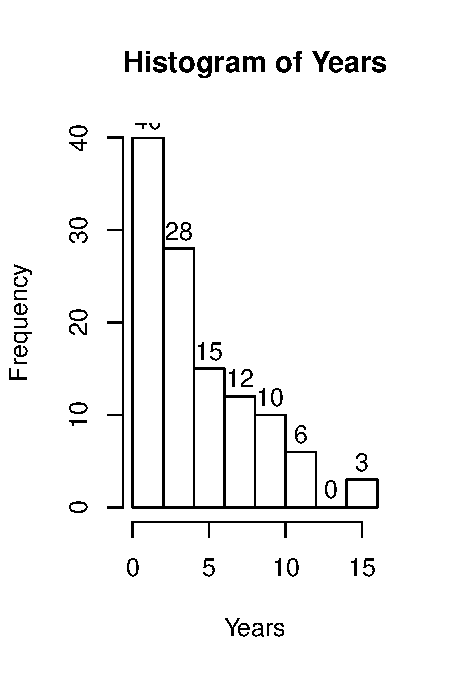
\includegraphics{GreenwoodBanner_files/figure-latex/Figure2-1-1.pdf}
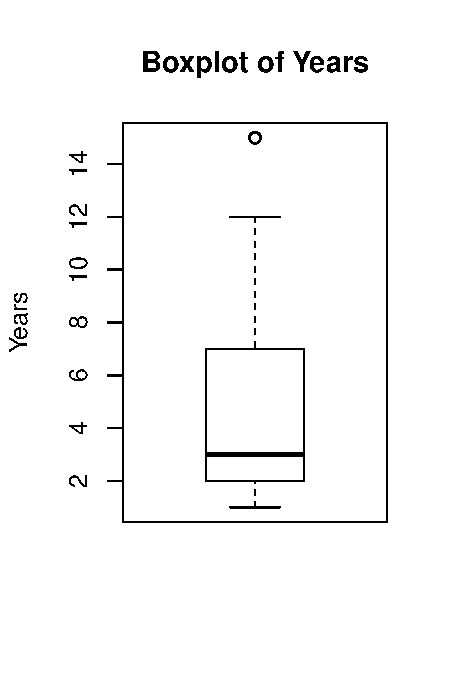
\includegraphics{GreenwoodBanner_files/figure-latex/Figure2-1-2.pdf}

The distribution appears to have a strong right skew with three
observations at 15 years flagged as potential outliers. You can only
tell that there are three observations and that they are at 15 by
looking at both plots -- the bar around 15 years in the histogram has a
count of three and the boxplot only shows a single point at 15 which is
actually three tied points at exactly 15 years plotted on top of each
other (we call this ``overplotting''). These three observations really
seem to be the upper edge of the overall pattern of a strongly right
skewed distribution, so even though they are flagged in the boxplot, we
likely would not want to remove them from our data set. In real data
sets, outliers are commonly encountered and the first step is to verify
that they were not errors in recording. The next step is to study their
impact on the statistical analyses performed, potentially considering
reporting results with and without the influential observation(s) in the
results. If the analysis is unaffected by the ``unusual'' observations,
then it matters little whether they are dropped or not. If they do
affect the results, then reporting both versions of results allows the
reader to judge the impacts for themselves. It is important to remember
that sometimes the outliers are the most interesting part of the data
set.

Often when statisticians think of distributions, we think of the smooth
underlying shape that led to the data set that is being displayed in the
histogram. Instead of binning up observations and making bars in the
histogram, we can estimate what is called a \textbf{\emph{density curve
}} as a smooth curve that represents the observed distribution of the
responses. Density curves can sometimes help us see features of the data
sets more clearly.

To understand the density curve, it is useful to initially see the
histogram and density curve together. The density curve is scaled so
that the total area\footnote{If you've taken calculus, you will know
  that the curve is being constructed so that the integral from
  \(-\infty\) to \(\infty\) is 1. If you don't know calculus, think of a
  rectangle with area of 1 based on its height and width. These cover
  the same area but the top of the region wiggles.} under the curve is
1. To make a comparable histogram, the y-axis needs to be scaled so that
the histogram is also on the ``density'' scale which makes the bar
heights required so that the proportion of the total data set in each
bar is represented by the area in each bar (remember that area is height
times width). So the height depends on the width of the bars and the
total area across all the bars has to be 1. In the \texttt{hist}
function, the \texttt{freq=F} to get density-scaled histogram bars. The
density curve is added to the histogram using the R code of
\texttt{lines(density())}, producing the result in Figure
\ref{fig:Figure2-2} with added modifications of options for \texttt{lwd}
(line width) and \texttt{col} (color) to make the plot more interesting.
You can see how the density curve somewhat matches the histogram bars
but deals with the bumps up and down and edges a little differently. We
can pick out the strong right skew using either display and will rarely
make both together.



\begin{Shaded}
\begin{Highlighting}[]
\KeywordTok{hist}\NormalTok{(MockJury$Years,}\DataTypeTok{freq=}\NormalTok{F,}\DataTypeTok{xlab=}\StringTok{"Years"}\NormalTok{,}\DataTypeTok{main=}\StringTok{"Histogram of Years"}\NormalTok{)}
\KeywordTok{lines}\NormalTok{(}\KeywordTok{density}\NormalTok{(MockJury$Years),}\DataTypeTok{lwd=}\DecValTok{3}\NormalTok{,}\DataTypeTok{col=}\StringTok{"red"}\NormalTok{)}
\end{Highlighting}
\end{Shaded}

\begin{figure}[htbp]
\centering
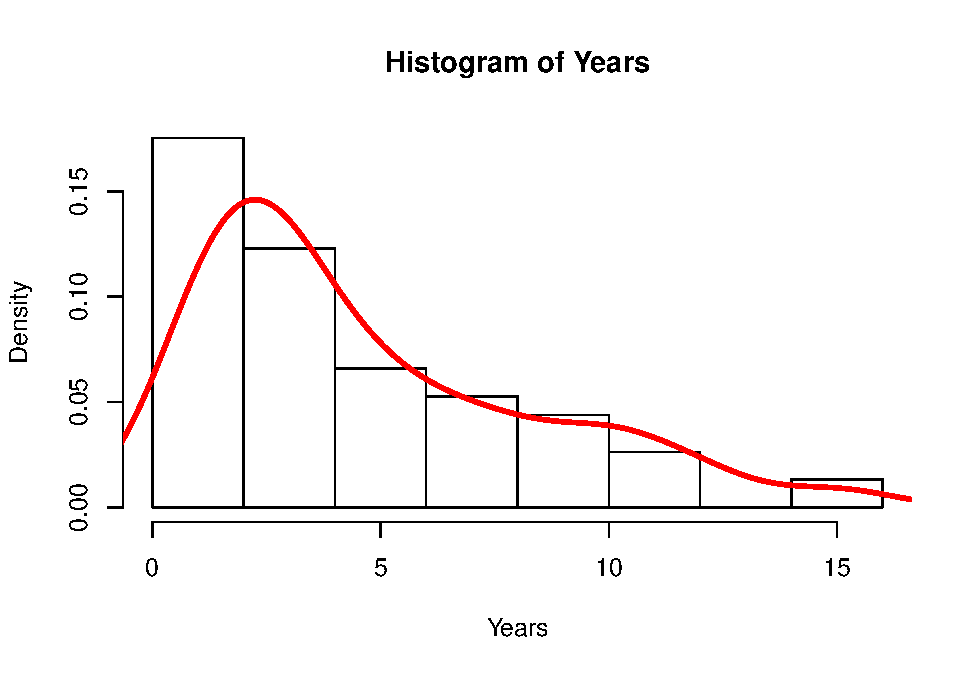
\includegraphics{GreenwoodBanner_files/figure-latex/Figure2-2-1.pdf}
\caption{\label{fig:Figure2-2}Histogram and density curve of Years data.}
\end{figure}

Histograms can be sensitive to the choice of the number of bars and even
the cut-offs used to define the bins for a given number of bars. Small
changes in the definition of cut-offs for the bins can have noticeable
impacts on the shapes observed but this does not impact density curves.
We are not going to tinker with the default choices for bars in
histogram as they are reasonably selected, but we can add information on
the original observations being included in each bar to better
understand the choices that \texttt{hist} is making. In the previous
display, we can add what is called a \textbf{\emph{rug}} to the plot,
were a tick mark is made on the x-axis for each observation. Because the
responses were provided as whole years (1, 2, 3, \ldots{}, 15), we need
to use a graphical technique called \textbf{\emph{jittering}} to add a
little noise\footnote{Jittering typically involves adding random
  variability to each observation that is uniformly distributed in a
  range determined based on the spacing of the function, the results
  will change. For more details, type \texttt{help(jitter)}\\
  in R.} to each observation so all the observations at each year value
do not plot as a single line. In Figure \ref{fig:Figure2-3}, the added
tick marks on the x-axis show the approximate locations of the original
observations. We can see how there are 3 observations at 15 (all were 15
and the noise added makes it possible to see them all). The limitations
of the histogram arise around the 10 year sentence area where there are
many responses at 10 years and just one at both 9 and 11 years, but the
histogram bars sort of miss this that aspect of the data set. The
density curve did show a small bump at 10 years. Density curves are,
however, not perfect and this one shows area for sentences less than 0
years which is not possible here.




\begin{Shaded}
\begin{Highlighting}[]
\KeywordTok{hist}\NormalTok{(MockJury$Years, }\DataTypeTok{freq=}\NormalTok{F, }\DataTypeTok{xlab=}\StringTok{"Years"}\NormalTok{,}
     \DataTypeTok{main=}\StringTok{"Histogram of Years with density curve and rug"}\NormalTok{)}
\KeywordTok{lines}\NormalTok{(}\KeywordTok{density}\NormalTok{(MockJury$Years),}\DataTypeTok{lwd=}\DecValTok{3}\NormalTok{,}\DataTypeTok{col=}\StringTok{"red"}\NormalTok{)}
\KeywordTok{rug}\NormalTok{(}\KeywordTok{jitter}\NormalTok{(MockJury$Years),}\DataTypeTok{col=}\StringTok{"blue"}\NormalTok{,}\DataTypeTok{lwd=}\DecValTok{2}\NormalTok{)}
\end{Highlighting}
\end{Shaded}

\begin{figure}[htbp]
\centering
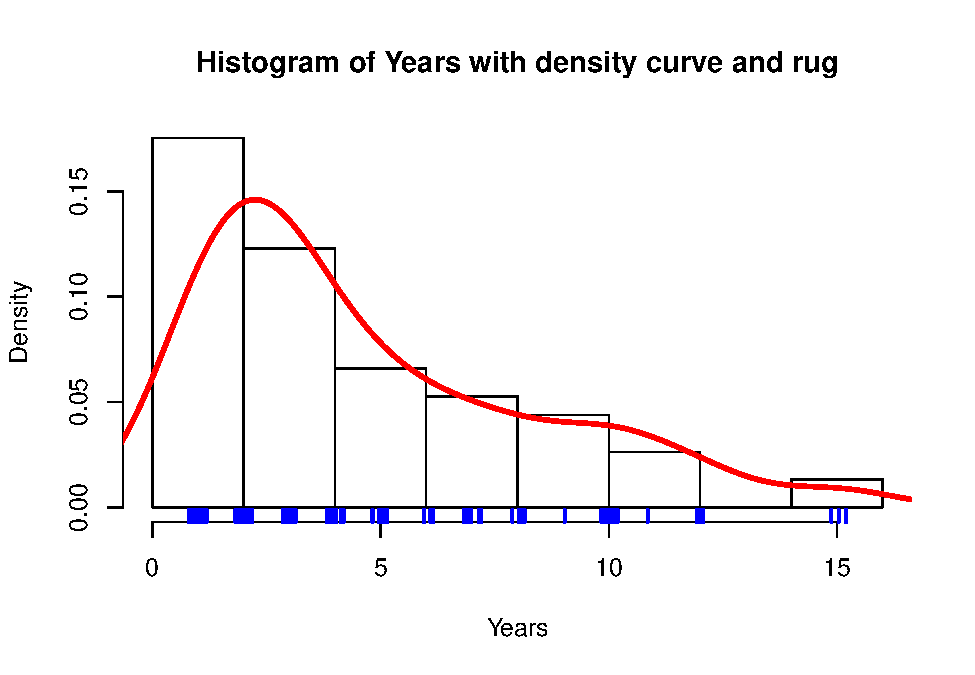
\includegraphics{GreenwoodBanner_files/figure-latex/Figure2-3-1.pdf}
\caption{\label{fig:Figure2-3}Histogram with density curve and rug plot of the jittered
responses.}
\end{figure}

The graphical tools we've just discussed are going to help us move to
comparing the distribution of responses across more than one group. We
will have two displays that will help us make these comparisons. The
simplest is \emph{the \textbf{side-by-side boxplot}}, where a boxplot is
displayed for each group of interest using the same y-axis scaling. In
R, we can use its \textbf{\emph{formula}} notation to see if the
response (\texttt{Years}) differs based on the group (\texttt{Attr}) by
using something like \texttt{Y\textasciitilde{}X} or, here,
\texttt{Years\textasciitilde{}Attr}. We also need to tell R where to
find the variables -- use the last option in the command,
\texttt{data=DATASETNAME} , to inform R of the data.frame to look in to
find the variables. In this example, \texttt{data=MockJury}. We will use
the formula and \texttt{data=...} options in almost every function we
use from here forward. Figure \ref{fig:Figure2-4} contains the
side-by-side boxplots showing right skew for all the groups, slightly
higher median and more variability for the \emph{Unattractive} group
along with some potential outliers indicated in two of the three groups.



\begin{Shaded}
\begin{Highlighting}[]
\KeywordTok{boxplot}\NormalTok{(Years~Attr,}\DataTypeTok{data=}\NormalTok{MockJury)}
\end{Highlighting}
\end{Shaded}

\begin{figure}[htbp]
\centering
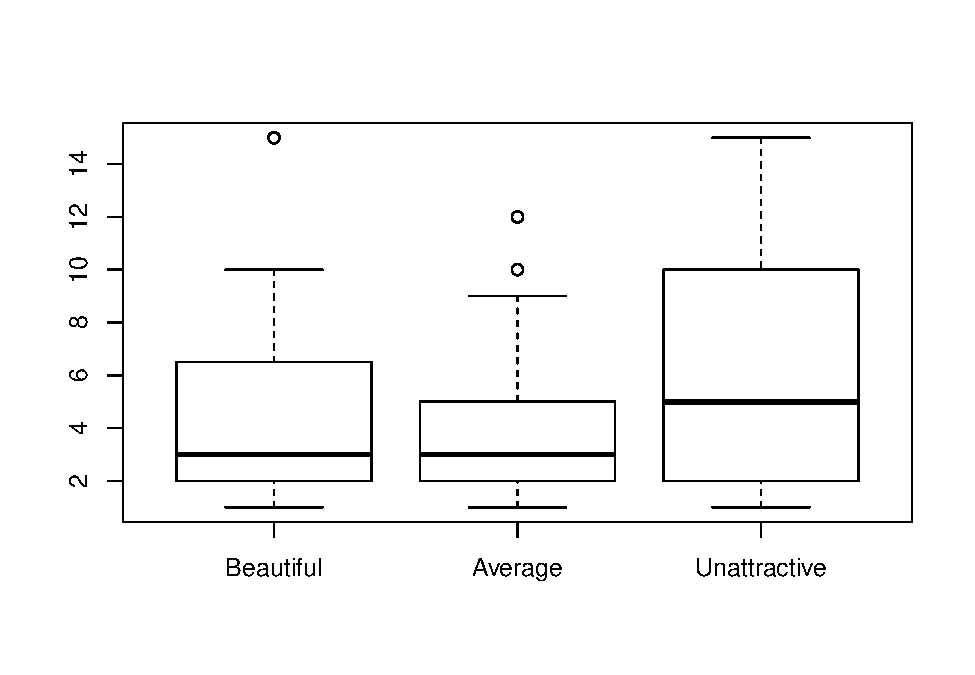
\includegraphics{GreenwoodBanner_files/figure-latex/Figure2-4-1.pdf}
\caption{\label{fig:Figure2-4}Side-by-side boxplot of Years based on picture groups.}
\end{figure}

The ``\textasciitilde{}'' (which is read as the \emph{tilde} symbol,
which you can find in the upper left corner of your keyboard) notation
will be used in two ways this semester. The formula use in R employed
previously declares that the response variable here is \emph{Years} and
the explanatory variable is \emph{Attr}. The other use for
``\textasciitilde{}'' is as shorthand for ``is distributed as'' and is
used in the context of \texttt{Y\textasciitilde{}N(0,1)}, which
translates (in statistics) to defining the random variable \emph{Y} as
following a Normal distribution\footnote{Remember the bell-shaped curve
  you encountered in introductory statistics? If not, you can see some
  at \url{https://en.wikipedia.org/wiki/Normal_distribution}} with mean
0 and standard deviation of 1. In the current situation, we could ask
whether the \texttt{Years} variable seems like it may follow a normal
distribution, in other words, is
\emph{Years}\texttt{\textasciitilde{}N(0,1)}? Since the responses are
right skewed with some groups having outliers, it is not reasonable to
assume that the \emph{Years} variable for any of the three groups may
follow a Normal distribution (more later on the issues this creates!).
Remember that\\
\(\mu\) and \(\sigma\) are parameters where\\
\(\mu\) (``mu'') is our standard symbol for the \textbf{\emph{population
mean}} and that \(\sigma\) (``sigma'') is the symbol of the\\
\textbf{\emph{population standard deviation}}.

\section{Beanplots}\label{section2-2}

The other graphical display for comparing multiple groups we will use is
a newer display called a \textbf{\emph{beanplot}} (Kampstra, 2008).
Figure \ref{fig:Figure2-5} shows an example of a beanplot that provides
a side-by-side display that contains the density curves, the original
observations that generated the density curve in a (jittered) rug-plot,
the mean of each group, and the overall mean of the entire data set. For
each group, the density curves are mirrored to aid in visual assessment
of the shape of the distribution, which makes a ``bean'' in some cases.
This mirroring also creates a shape that resembles a violin with skewed
distributions so this display has also been called a ``violin plot''.
The innovation in the beanplot is to add bold horizontal lines at the
mean for each group. It also adds a lighter dashed line for the overall
mean. All together this plot shows us information on the center (mean),
spread, and shape of the distributions of the responses. Our inferences
typically focus on the means of the groups and this plot allows us to
compare those across the groups while gaining information on the shapes
of the distributions of responses in each group.

To use the \texttt{beanplot} function we need to install and load the
\texttt{beanplot} package. The function works like the boxplot used
previously except that options for \texttt{log}, \texttt{col}, and
\texttt{method} need to be specified. Use these\footnote{Well, you can
  use other colors (try ``lightblue'' for example), but I think bisque
  looks nice in these plots.} options for any beanplots you make:
\texttt{log="",\ col="bisque",\ method="jitter"}




\begin{Shaded}
\begin{Highlighting}[]
\KeywordTok{require}\NormalTok{(beanplot)}
\KeywordTok{beanplot}\NormalTok{(Years~Attr,}\DataTypeTok{data=}\NormalTok{MockJury,}\DataTypeTok{log=}\StringTok{""}\NormalTok{,}\DataTypeTok{col=}\StringTok{"bisque"}\NormalTok{,}\DataTypeTok{method=}\StringTok{"jitter"}\NormalTok{)}
\end{Highlighting}
\end{Shaded}

\begin{figure}[htbp]
\centering
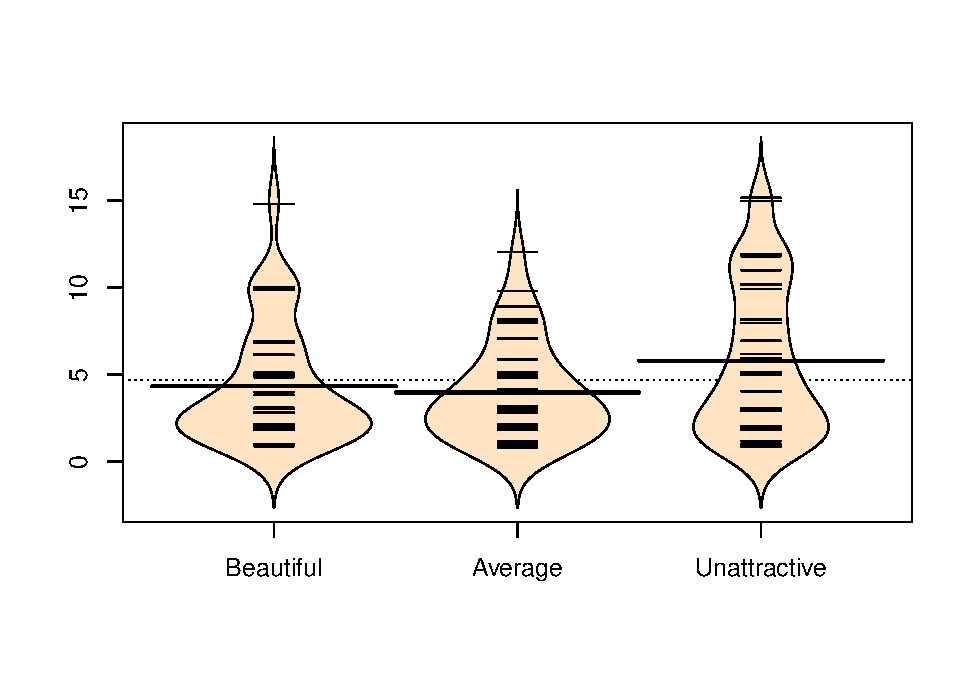
\includegraphics{GreenwoodBanner_files/figure-latex/Figure2-5-1.pdf}
\caption{\label{fig:Figure2-5}Beanplot of Years by picture group. Long, bold lines
correspond to mean of each group.}
\end{figure}

Figure \ref{fig:Figure2-5} reinforces the strong right skews that were
also detected in the boxplots previously. The three large sentences of
15 years can now be clearly identified, with one in the \emph{Beautiful}
group and two in the \emph{Unattractive} group. The \emph{Unattractive}
group seems to have more high observations than the other groups even
though the \emph{Beautiful} group had the largest number of observations
around 10years. The mean sentence was highest for the
\emph{Unattractive} group and the difference in the means between
\emph{Beautiful} and \emph{Average} was small.

In this example, it appears that the mean for \emph{Unattractive} is
larger than the other two groups. But is this difference real? We will
never know the answer to that question, but we can assess how likely we
are to have seen a result as extreme or more extreme than our result,
assuming that there is no difference in the means of the groups. And if
the observed result is (extremely) unlikely to occur, then we can reject
the hypothesis that the groups have the same mean and conclude that
there is evidence of a real difference. To start exploring whether there
are differences in the means, we need to have numerical values to
compare. We can get means and standard deviations by groups easily using
the same formula notation with the \texttt{mean} and \texttt{sd}
functions if the \texttt{mosaic} package is loaded.

\begin{Shaded}
\begin{Highlighting}[]
\KeywordTok{mean}\NormalTok{(Years ~}\StringTok{ }\NormalTok{Attr, }\DataTypeTok{data =} \NormalTok{MockJury)}
\end{Highlighting}
\end{Shaded}

\begin{verbatim}
##    Beautiful      Average Unattractive 
##     4.333333     3.973684     5.810811
\end{verbatim}

\begin{Shaded}
\begin{Highlighting}[]
\KeywordTok{sd}\NormalTok{(Years ~}\StringTok{ }\NormalTok{Attr, }\DataTypeTok{data =} \NormalTok{MockJury)}
\end{Highlighting}
\end{Shaded}

\begin{verbatim}
##    Beautiful      Average Unattractive 
##     3.405362     2.823519     4.364235
\end{verbatim}

We can also use the \texttt{favstats} function to get those summaries
and others.

\begin{Shaded}
\begin{Highlighting}[]
\KeywordTok{favstats}\NormalTok{(Years ~}\StringTok{ }\NormalTok{Attr, }\DataTypeTok{data =} \NormalTok{MockJury)}
\end{Highlighting}
\end{Shaded}

\begin{verbatim}
##           Attr min Q1 median   Q3 max     mean       sd  n missing
## 1    Beautiful   1  2      3  6.5  15 4.333333 3.405362 39       0
## 2      Average   1  2      3  5.0  12 3.973684 2.823519 38       0
## 3 Unattractive   1  2      5 10.0  15 5.810811 4.364235 37       0
\end{verbatim}

Based on these results, we can see that there is an estimated difference
of almost 2 years in the mean sentence between \emph{Average} and
\emph{Unattractive} groups. Because there are three groups being
compared in this study, we will have to wait until Chapter 3 and the
One-Way ANOVA test to fully assess evidence related to some difference
among the three groups. For now, we are going to focus on comparing the
mean \emph{Years} between \emph{Average} and \emph{Unattractive} groups
-- which is a \textbf{\emph{2 independent sample mean}} situation and
something you should have seen before. Remember that the ``independent''
sample part of this refers to observations that are independently
observed for the two groups as opposed to the paired sample situation
that you may have explored where one observation from the first group is
related to an observation in the second group (repeated measures on the
same person or the famous ``twin'' studies with one twin assigned to
each group).

Here we are going to use the ``simple'' two independent group scenario
to review some basic statistical concepts and connect two different
frameworks for conducting statistical inference: randomization and
parametric inference techniques. \textbf{\emph{Parametric}} statistical
methods involve making assumptions about the distribution of the
responses and obtaining confidence intervals and/or p-values using a
\emph{named} distribution (like the z or \(t\)-distributions). Typically
these results are generated using formulas and looking up areas under
curves or cutoffs using a table or a computer.
\textbf{\emph{Randomization}}-based statistical methods use a computer
to shuffle, sample, or simulate observations in ways that allow you to
obtain distributions of possible results to find areas and cutoffs
without resorting to using tables and named distributions. Randomization
methods are what are called \textbf{\emph{nonparametric}} methods that
often make fewer assumptions (they are \textbf{\emph{not free of
assumptions}}!) and so can handle a larger set of problems more easily
than parametric methods. When the assumptions involved in the parametric
procedures are met by a data set, the randomization methods often
provide very similar results to those provided by the parametric
techniques. To be a more sophisticated statistical consumer, it is
useful to have some knowledge of both of these approaches to statistical
inference and the fact that they can provide similar results might
deepen your understanding of both approaches.

We will start with comparing the \emph{Average} and \emph{Unattractive}
groups to compare these two ways of doing inference. We could remove the
\emph{Beautiful} group observations in a spreadsheet program and read
that new data set back into R, but it is actually pretty easy to use R
to do data management once the data set is loaded. To remove the
observations that came from the \emph{Beautiful} group, we are going to
generate a new variable that we will call \texttt{NotBeautiful} that is
true when observations came from another group (\emph{Average} or
\emph{Unattractive}) and false for observations from the
\emph{Beautiful} group. To do this, we will apply the \textbf{\emph{not
equal}} logical function (\texttt{!=} ) to the variable \texttt{Attr},
inquiring whether it was different from the \texttt{"Beautiful"} level.
You can see the content of the new variable in the output:

\begin{Shaded}
\begin{Highlighting}[]
\NormalTok{MockJury$NotBeautiful <-}\StringTok{ }\NormalTok{MockJury$Attr !=}\StringTok{ "Beautiful"}
\NormalTok{MockJury$NotBeautiful}
\end{Highlighting}
\end{Shaded}

\begin{verbatim}
##   [1] FALSE FALSE FALSE FALSE FALSE FALSE FALSE FALSE FALSE FALSE FALSE
##  [12] FALSE FALSE FALSE FALSE FALSE FALSE FALSE FALSE FALSE FALSE  TRUE
##  [23]  TRUE  TRUE  TRUE  TRUE  TRUE  TRUE  TRUE  TRUE  TRUE  TRUE  TRUE
##  [34]  TRUE  TRUE  TRUE  TRUE  TRUE  TRUE  TRUE  TRUE  TRUE  TRUE  TRUE
##  [45]  TRUE  TRUE  TRUE  TRUE  TRUE  TRUE  TRUE  TRUE  TRUE  TRUE  TRUE
##  [56]  TRUE  TRUE  TRUE  TRUE  TRUE  TRUE  TRUE  TRUE  TRUE  TRUE  TRUE
##  [67]  TRUE  TRUE  TRUE  TRUE  TRUE  TRUE  TRUE  TRUE  TRUE  TRUE FALSE
##  [78] FALSE FALSE FALSE FALSE FALSE FALSE FALSE FALSE FALSE FALSE FALSE
##  [89] FALSE FALSE FALSE FALSE FALSE FALSE  TRUE  TRUE  TRUE  TRUE  TRUE
## [100]  TRUE  TRUE  TRUE  TRUE  TRUE  TRUE  TRUE  TRUE  TRUE  TRUE  TRUE
## [111]  TRUE  TRUE  TRUE  TRUE
\end{verbatim}

This new variable is only FALSE for the \emph{Beautiful} responses as we
can see if we compare some of the results from the original and new
variable:

\begin{Shaded}
\begin{Highlighting}[]
\KeywordTok{head}\NormalTok{(}\KeywordTok{data.frame}\NormalTok{(MockJury$Attr, MockJury$NotBeautiful))}
\end{Highlighting}
\end{Shaded}

\begin{verbatim}
##   MockJury.Attr MockJury.NotBeautiful
## 1     Beautiful                 FALSE
## 2     Beautiful                 FALSE
## 3     Beautiful                 FALSE
## 4     Beautiful                 FALSE
## 5     Beautiful                 FALSE
## 6     Beautiful                 FALSE
\end{verbatim}

\begin{Shaded}
\begin{Highlighting}[]
\KeywordTok{tail}\NormalTok{(}\KeywordTok{data.frame}\NormalTok{(MockJury$Attr, MockJury$NotBeautiful))}
\end{Highlighting}
\end{Shaded}

\begin{verbatim}
##     MockJury.Attr MockJury.NotBeautiful
## 109       Average                  TRUE
## 110       Average                  TRUE
## 111       Average                  TRUE
## 112       Average                  TRUE
## 113       Average                  TRUE
## 114       Average                  TRUE
\end{verbatim}

To get rid of one of the groups, we need to learn a little bit about
data management in R. \textbf{\emph{Brackets}} \texttt{({[},\ {]})} are
used to modify the rows or columns in a data.frame with entries before
the comma operating on rows and entries after the comma on the columns.
For example, if you want to see the results for the 5\(^{th}\) subject,
you can reference the 5\(^{th}\) row of the data.frame using
\texttt{{[}5,\ {]}} after the data.frame name:

\begin{Shaded}
\begin{Highlighting}[]
\NormalTok{MockJury[}\DecValTok{5}\NormalTok{,]}
\end{Highlighting}
\end{Shaded}

\begin{verbatim}
##        Attr    Crime Years Serious exciting calm independent sincere warm
## 5 Beautiful Burglary     7       9        1    1           5       1    8
##   phyattr sociable kind intelligent strong sophisticated happy ownPA
## 5       8        9    4           7      9             9     8     7
##   NotBeautiful
## 5        FALSE
\end{verbatim}

We could just extract the \emph{Years} response for the 5\(^{th}\)
subject by incorporating information on the row and column of interest
(\texttt{Years} is the 3\(^{rd}\) column):

\begin{Shaded}
\begin{Highlighting}[]
\NormalTok{MockJury[}\DecValTok{5}\NormalTok{,}\DecValTok{3}\NormalTok{]}
\end{Highlighting}
\end{Shaded}

\begin{verbatim}
## [1] 7
\end{verbatim}

In R, we can use logical vectors to keep any rows of the data.frame
where the variable is true and drop any rows where it is false by
placing the logical variable in the first element of the brackets. The
reduced version of the data set should be saved with a different name
such as \texttt{MockJury2} that is used here to reduce the chances of
confusing it with the previous full data set:

\begin{Shaded}
\begin{Highlighting}[]
\NormalTok{MockJury2 <-}\StringTok{ }\NormalTok{MockJury[MockJury$NotBeautiful,]}
\end{Highlighting}
\end{Shaded}

You will always want to check that the correct observations were dropped
either using \texttt{View(MockJury2)} or by doing a quick summary of the
\texttt{Attr} variable in the new data.frame.

\begin{Shaded}
\begin{Highlighting}[]
\KeywordTok{summary}\NormalTok{(MockJury2$Attr)}
\end{Highlighting}
\end{Shaded}

\begin{verbatim}
##    Beautiful      Average Unattractive 
##            0           38           37
\end{verbatim}

It ends up that R remembers the \emph{Beautiful} category even though
there are 0 observations in it now and that can cause us some problems.
When we remove a group of observations, we sometimes need to clean up
categorical variables to just reflect the categories that are present.
The \texttt{factor} function creates categorical variables based on the
levels of the variables that are observed and is useful to run here to
clean up \texttt{Attr}.

\begin{Shaded}
\begin{Highlighting}[]
\NormalTok{MockJury2$Attr <-}\StringTok{ }\KeywordTok{factor}\NormalTok{(MockJury2$Attr) }
\KeywordTok{summary}\NormalTok{(MockJury2$Attr)}
\end{Highlighting}
\end{Shaded}

\begin{verbatim}
##      Average Unattractive 
##           38           37
\end{verbatim}

Now if we remake the boxplots and beanplots, they only contain results
for the two groups of interest here as seen in Figure
\ref{fig:Figure2-6}.




\begin{Shaded}
\begin{Highlighting}[]
\KeywordTok{boxplot}\NormalTok{(Years ~}\StringTok{ }\NormalTok{Attr,}\DataTypeTok{data=}\NormalTok{MockJury2) }
\KeywordTok{beanplot}\NormalTok{(Years ~}\StringTok{ }\NormalTok{Attr,}\DataTypeTok{data=}\NormalTok{MockJury2,}\DataTypeTok{log=}\StringTok{""}\NormalTok{,}\DataTypeTok{col=}\StringTok{"bisque"}\NormalTok{,}\DataTypeTok{method=}\StringTok{"jitter"}\NormalTok{)}
\end{Highlighting}
\end{Shaded}

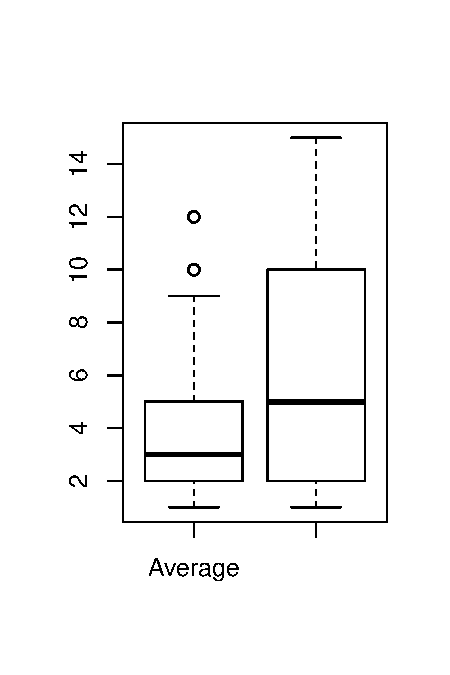
\includegraphics{GreenwoodBanner_files/figure-latex/Figure2-6-1.pdf}
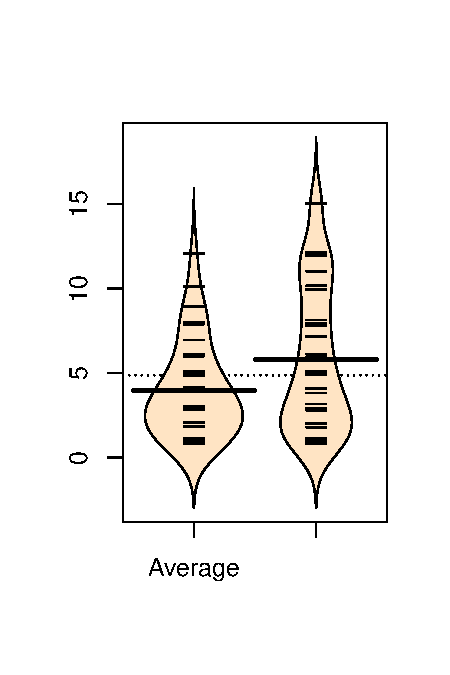
\includegraphics{GreenwoodBanner_files/figure-latex/Figure2-6-2.pdf}

The two-sample mean techniques you learned in your previous course all
start with comparing the means the two groups. We can obtain the two
means using the \texttt{mean} function or directly obtain the difference
in the means using the \texttt{diffmean} function (both require the
\texttt{mosaic} package). The \texttt{diffmean} function provides
\(\bar{x}_{Unattractive} - \bar{x}_{Average}\) where \(\bar{x}\) (read
as ``x-bar'') is the sample mean ofobservations in the subscripted
group. Note that there are two directions that you could compare the
means and this function chooses to take the mean from the second group
name \emph{alphabetically} and subtract the mean from the first
alphabetical group name. It is always good to check the direction of
this calculation as having a difference of \(-1.84\) years versus
\(1.84\) years could be important.

\begin{Shaded}
\begin{Highlighting}[]
\KeywordTok{mean}\NormalTok{(Years ~}\StringTok{ }\NormalTok{Attr, }\DataTypeTok{data=}\NormalTok{MockJury2)}
\end{Highlighting}
\end{Shaded}

\begin{verbatim}
##      Average Unattractive 
##     3.973684     5.810811
\end{verbatim}

\begin{Shaded}
\begin{Highlighting}[]
\KeywordTok{diffmean}\NormalTok{(Years ~}\StringTok{ }\NormalTok{Attr, }\DataTypeTok{data=}\NormalTok{MockJury2)}
\end{Highlighting}
\end{Shaded}

\begin{verbatim}
## diffmean 
## 1.837127
\end{verbatim}

\section{Models, hypotheses, and permutations for the 2 sample mean
situation}\label{section2-3}

There appears to be some evidence that the \emph{Unattractive} group is
getting higher average lengths of sentences from the prisoner ``jurors''
than the \emph{Average} group, but we want to make sure that the
difference is real -- that there is evidence to reject the assumption
that the means are the same ``in the population''. First, a
\textbf{\emph{null hypothesis}}\footnote{The hypothesis of no difference
  that is typically generated in the hopes of being rejected in favor of
  the alternative hypothesis which contains the sort of difference that
  is of interest in the application.} which defines a \textbf{\emph{null
model}}\footnote{The null model is the statistical model that is implied
  by the chosen null hypothesis. Here, a null hypothesis of no
  difference translates to having a model with the same mean for both
  groups.} needs to be determined in terms of \textbf{\emph{parameters}}
(the true values in the population). The research question should help
you determine the form of the hypotheses for the assumed population. In
the 2 independent sample mean problem, the interest is in testing a null
hypothesis of \(H_0: \mu_1 = \mu_2\) versus the alternative hypothesis
of \(H_A: \mu_1 \ne \mu_2\), where \(\mu_1\) is the parameter for the
true mean of the first group and \(\mu_2\) is the parameter for the true
mean of the second group. The alternative hypothesis involves assuming a
statistical model for the \(i^{th} (i=1,\ldots,n_j)\) response from the
\(j^{th} (j=1,2)\) group, \(\boldsymbol{y}_{ij}\), that involves
modeling it as \(y_{ij} = \mu_j + \epsilon_{ij}\), where we assume that
\(\epsilon_{ij} \sim N(0,\sigma^2)\). For the moment, focus on the
models that either assume the means are the same (null) or different
(alternative), which imply:

\begin{itemize}
\item
  Null Model: \(y_{ij} = \mu + \epsilon_{ij}\) There is \textbf{no}
  difference in \textbf{true} means for the two groups.
\item
  Alternative Model: \(y_{ij} = \mu_j + \epsilon_{ij}\) There is
  \textbf{a} difference in \textbf{true} means for the two groups.
\end{itemize}

Suppose we are considering the alternative model for the 4th observation
(\(i=4\)) from the second group (\(j=2\)), then the model for this
observation is \(y_{42} = \mu_2 +\epsilon_{42}\), that defines the
response as coming from the true mean for the second group plus a random
error term for that observation, \(\epsilon_{42}\). For, say, the 5th
observation from the first group (\(j=1\)), the model is
\(y_{51} = \mu_1 +\epsilon_{51}\). If we were working with the null
model, the mean is always the same (\(\mu\)) - the group specified does
not change the mean we use for that observation.

It can be helpful to think about the null and alternative models
graphically. By assuming the null hypothesis is true (means are equal)
and that the random errors around the mean follow a normal distribution,
we assume that the truth is as displayed in the left panel of Figure
\ref{fig:Figure2-7} -- two normal distributions with the same mean and
variability. The alternative model allows the two groups to potentially
have different means, such as those displayed in the right panel of
Figure \ref{fig:Figure2-7} where the second group has a larger mean.
Note that in this scenario, we assume that the observations all came
from the same distribution except that they had different means.
Depending on the statistical procedure we are using, we basically are
going to assume that the observations (\(y_{ij}\)) either were generated
as samples from the null or alternative model. You can imagine drawing
observations at random from the pictured distributions. For hypothesis
testing, the null model is assumed to be true and then the unusualness
of the actual result is assessed relative to that assumption. In
hypothesis testing, we have to decide if we have enough evidence to
reject the assumption that the null model (or hypothesis) is true. If we
reject the null hypothesis, then we would conclude that the other model
considered (the alternative model) is more reasonable. The researchers
obviously would have hoped to encounter some sort of noticeable
difference in the sentences provided for the different pictures and been
able to find enough evidence to reject the null model where the groups
``look the same''.





\begin{figure}
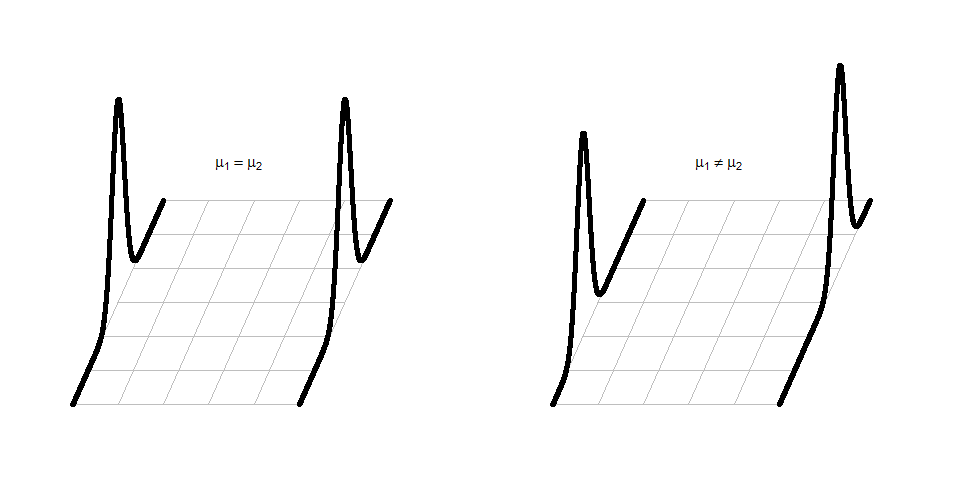
\includegraphics[width=13.33in]{chapter1_files/image015} \caption{Illustration of the assumed situations under the null
(left) and a single possibility that could occur if the alternative were
true (right) and the true means were different.}\label{fig:Figure2-7}
\end{figure}

In statistical inference, null hypotheses (and their implied models) are
set up as ``straw men'' with every interest in rejecting them even
though we assume they are true to be able to assess the evidence against
them. Consider the original study design here, the pictures were
randomly assigned to the subjects. If the null hypothesis were true,
then we would have no difference in the population means of the groups.
And this would apply if we had done a different random assignment of the
pictures to the subjects. So let's try this: assume that the null
hypothesis is true and randomly re-assign the treatments (pictures) to
the observations that were obtained. In other words, keep the sentences
(\emph{Years}) the same and shuffle the group labels randomly. The
technical term for this is doing a \textbf{\emph{permutation}} (a random
shuffling of the treatments relative to the responses). If the null is
true and the means in the two groups are the same, then we should be
able to re-shuffle the groups to the observed sentences (\emph{Years})
and get results similar to those we actually observed. If the null is
false and the means are really different in the two groups, then what we
observed should differ from what we get under other random permutations.
The differences between the two groups should be more noticeable in the
observed data set than in (most) of the shuffled data sets. It helps to
see an example of a permutation of the labels to understand what this
means here.

In the \texttt{mosaic} package, the \texttt{shuffle} function allows us
to easily perform a permutation\footnote{We'll see the \texttt{shuffle}
  function in a more common usage below; while the code to generate
  \texttt{Perm1} is provided, it isn't something to worry about right
  now.}. Just one time, we can explore what a permutation of the
treatment labels could look like in the \texttt{PermutedAttr} variable
below. Note that the \texttt{Years} are held in the same place the group
labels are shuffled.

\begin{Shaded}
\begin{Highlighting}[]
\KeywordTok{set.seed}\NormalTok{(}\DecValTok{1234}\NormalTok{)}
\end{Highlighting}
\end{Shaded}

\begin{Shaded}
\begin{Highlighting}[]
\NormalTok{Perm1 <-}\StringTok{ }\KeywordTok{with}\NormalTok{(MockJury2,}\KeywordTok{data.frame}\NormalTok{(Years,Attr,}\DataTypeTok{PermutedAttr=}\KeywordTok{shuffle}\NormalTok{(Attr)))}
\NormalTok{Perm1}
\end{Highlighting}
\end{Shaded}

\begin{verbatim}
##    Years         Attr PermutedAttr
## 1      1 Unattractive Unattractive
## 2      4 Unattractive      Average
## 3      3 Unattractive      Average
## 4      2 Unattractive      Average
## 5      8 Unattractive      Average
## 6      8 Unattractive      Average
## 7      1 Unattractive Unattractive
## 8      1 Unattractive Unattractive
## 9      5 Unattractive      Average
## 10     7 Unattractive Unattractive
## 11     1 Unattractive      Average
## 12     5 Unattractive Unattractive
## 13     2 Unattractive Unattractive
## 14    12 Unattractive      Average
## 15    10 Unattractive      Average
## 16     1 Unattractive      Average
## 17     6 Unattractive Unattractive
## 18     2 Unattractive      Average
## 19     5 Unattractive Unattractive
## 20    12 Unattractive Unattractive
## 21     6 Unattractive      Average
## 22     3 Unattractive      Average
## 23     8 Unattractive      Average
## 24     4 Unattractive Unattractive
## 25    10 Unattractive Unattractive
## 26    10 Unattractive      Average
## 27    15 Unattractive Unattractive
## 28    15 Unattractive      Average
## 29     3 Unattractive      Average
## 30     3 Unattractive      Average
## 31     3 Unattractive Unattractive
## 32    11 Unattractive      Average
## 33    12 Unattractive      Average
## 34     2 Unattractive Unattractive
## 35     1 Unattractive Unattractive
## 36     1 Unattractive Unattractive
## 37    12 Unattractive      Average
## 38     5      Average Unattractive
## 39     5      Average Unattractive
## 40     4      Average Unattractive
## 41     3      Average Unattractive
## 42     6      Average      Average
## 43     4      Average      Average
## 44     9      Average      Average
## 45     8      Average Unattractive
## 46     3      Average      Average
## 47     2      Average Unattractive
## 48    10      Average      Average
## 49     1      Average Unattractive
## 50     1      Average Unattractive
## 51     3      Average Unattractive
## 52     1      Average      Average
## 53     3      Average      Average
## 54     5      Average      Average
## 55     8      Average Unattractive
## 56     3      Average      Average
## 57     1      Average      Average
## 58     1      Average Unattractive
## 59     1      Average      Average
## 60     2      Average      Average
## 61     2      Average Unattractive
## 62     1      Average      Average
## 63     1      Average Unattractive
## 64     2      Average Unattractive
## 65     3      Average Unattractive
## 66     4      Average Unattractive
## 67     5      Average      Average
## 68     3      Average Unattractive
## 69     3      Average      Average
## 70     3      Average      Average
## 71     2      Average Unattractive
## 72     7      Average Unattractive
## 73     6      Average Unattractive
## 74    12      Average Unattractive
## 75     8      Average      Average
\end{verbatim}

If you count up the number of subjects in each group by counting the
number of times each label (Average, Unattractive) occurs, it is the
same in both the \texttt{Attr} and \texttt{PermutedAttr} columns.
Permutations involve randomly re-ordering the values of a variable --
here the \texttt{Attr} group labels -- without changing the content of
the variable. This result can also be generated using what is called
\textbf{\emph{sampling without replacement}}: sequentially select \(n\)
labels from the original variable, removing each used label and making
sure that each original \texttt{Attr} label is selected once and only
once. The new, randomly selected order of selected labels provides the
permuted labels. Stepping through the process helps to understand how it
works: after the initial random sample of one label, there would
\(n - 1\) choices possible; on the \(n^{th}\) selection, there would
only be one label remaining to select. This makes sure that all original
labels are re-used but that the order is random. Sampling without
replacement is like picking names out of a hat, one-at-a-time, and not
putting the names back in after they are selected. It is an exhaustive
process for all the original observations. \textbf{\emph{Sampling with
replacement}} , in contrast, involves sampling from the specified list
with each observation having an equal chance of selection for each
sampled observation -- in other words, observations can be selected more
than once. This is like picking \(n\) names out of a hat that contains
\(n\) names, except that every time a name is selected, it goes back
into the hat -- we'll use this technique in Section \ref{section2-8} to
do what is called \textbf{\emph{bootstrapping}}. Both sampling
mechanisms can be used to generate inferences but each has particular
situations where they are most useful. For hypothesis testing, we will
use permutations (sampling without replacement).

The comparison of the beanplots for the real data set and permuted
version of the labels is what is really interesting (Figure
\ref{fig:Figure2-8}). The original difference in the sample means of the
two groups was 1.84 years (Unattractive minus Average). The sample means
are the \textbf{\emph{statistics}}\\
that estimate the parameters for the true means of the two groups. In
the permuted data set, the difference in the means is 1.15 years in the
opposite direction (Average had a higher mean than Unattractive in the
permuted data).

\begin{Shaded}
\begin{Highlighting}[]
\KeywordTok{mean}\NormalTok{(Years ~}\StringTok{ }\NormalTok{PermutedAttr, }\DataTypeTok{data=}\NormalTok{Perm1)}
\end{Highlighting}
\end{Shaded}

\begin{verbatim}
##      Average Unattractive 
##     5.447368     4.297297
\end{verbatim}

\begin{Shaded}
\begin{Highlighting}[]
\KeywordTok{diffmean}\NormalTok{(Years ~}\StringTok{ }\NormalTok{PermutedAttr, }\DataTypeTok{data=}\NormalTok{Perm1)}
\end{Highlighting}
\end{Shaded}

\begin{verbatim}
##  diffmean 
## -1.150071
\end{verbatim}




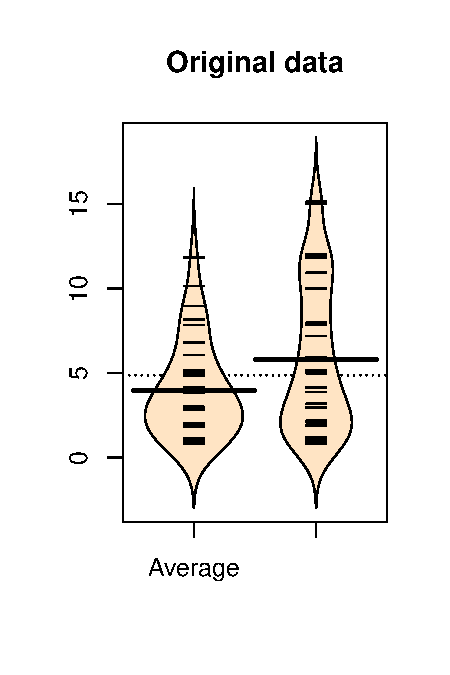
\includegraphics{GreenwoodBanner_files/figure-latex/Figure2-8-1.pdf}
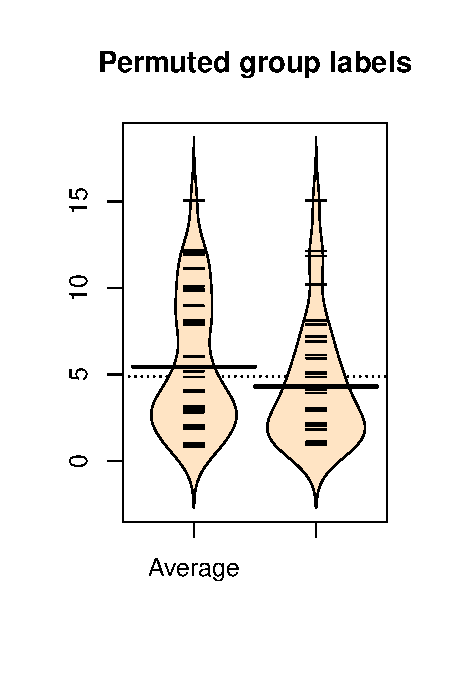
\includegraphics{GreenwoodBanner_files/figure-latex/Figure2-8-2.pdf}

These results suggest that the observed difference was larger than what
we got when we did a single permutation although it was only a little
bit larger than a difference we could observe in permutations if we
ignore the difference in directions. Conceptually, permuting
observations between group labels is consistent with the null hypothesis
-- this is a technique to generate results that we might have gotten if
the null hypothesis were true since the responses are the same in the
two groups if the null is true. We just need to repeat the permutation
process many times and track how unusual our observed result is relative
to this distribution of potential responses if the null were true. If
the observed differences are unusual relative to the results under
permutations, then there is evidence against the null hypothesis, the
null hypothesis should be rejected ( Reject \(H_0\)), and a conclusion
should be made, in the direction of the alternative hypothesis, that
there is evidence that the true means differ. If the observed
differences are similar to (or at least not unusual relative to) what we
get under random shuffling under the null model, we would have a tough
time concluding that there is any real difference between the groups
based on our observed data set.

\section{Permutation testing for the 2 sample mean
situation}\label{section2-4}

In any testing situation, you must define some function of the
observations that gives us a single number that addresses our question
of interest. This quantity is called a \textbf{\emph{test statistic}}.
These often take on complicated forms and have names like \(t\) or \(z\)
statistics that relate to their parametric (named) distributions so we
know where to look up \textbf{\emph{p-values}}\footnote{P-values are the
  probability of obtaining a result as extreme as or more extreme than
  we observed given that the null hypothesis is true.}. In randomization
settings, they can have simpler forms because we use the data set to
find the distribution of the statistic and don't need to rely on a named
distribution. We will label our test statistic \textbf{\emph{T}} (for
\textbf{T} statistic) unless the test statistic has a commonly used
name. Since we are interested in comparing the means of the two groups,
we can define

\[T=\bar{x}_{Unattractive}-\bar{x}_{Average},\]

which coincidentally is what the\texttt{diffmean} function provided us
previously. We label our \textbf{\emph{observed test statistic}} (the
one from the original data set) as

\[T_{obs}=\bar{x}_{Unattractive}-\bar{x}_{Average},\]

which happened to be 1.84 years here. We will compare this result to the
results for the test statistic that we obtain from permuting the group
labels. To denote permuted results, we will add a * to the labels:

\[T^*=\bar{x}_{Unattractive}-\bar{x}_{Average^*}.\]

We then compare the
\(T_{obs}=\bar{x}_{Unattractive}-\bar{x}_{Average} = 1.84\) to the
distribution of results that are possible for the permuted results
(\(T^*\)) which corresponds to assuming the null hypothesis is true.

We need to consider lots of permutations to do a permutation test. In
contrast to your introductory statistics course where, if you did this,
it was just a click away, we are going to learn what was going on under
the hood. Specifically, we need a \textbf{\emph{for loop}} in R to be
able to repeatedly generate the permuted data sets and record \(T^*\)
for each one. Loops are a basic programming task that make randomization
methods possible as well as potentially simplifying any repetitive
computing task. To write a ``for loop'', we need to choose how many
times we want to do the loop (call that \texttt{B}) and decide on a
counter to keep track of where we are at in the loops (call that
\texttt{b}, which goes from 1 up to \texttt{B}). The simplest loop just
involves printing out the index, \texttt{print(b)} at each step. This is
our first use of curly braces, \{ and\}, that are used to group the code
we want to repeatedly run as we proceed through the loop. By typing the
following code in the script window and then highlighting it all and
hitting the run button, R will go through the loop 5 times, printing out
the counter:

\begin{verbatim}
B <- 5
for (b in (1:B)){
  print(b)
}
\end{verbatim}

Note that when you highlight and run the code, it will look about the
same with ``+'' printed after the first line to indicate that all the
code is connected when it appears in the console, looking like this:

\begin{Shaded}
\begin{Highlighting}[]
\NormalTok{>}\StringTok{ }\NormalTok{for(b in (}\DecValTok{1}\NormalTok{:B))\{}
\NormalTok{+}\StringTok{   }\KeywordTok{print}\NormalTok{(b)}
\NormalTok{+\}}
\end{Highlighting}
\end{Shaded}

When you run these three lines ofcode, the console will show you the
following output:

\begin{Shaded}
\begin{Highlighting}[]
\NormalTok{[}\DecValTok{1}\NormalTok{] }\DecValTok{1}
\NormalTok{[}\DecValTok{1}\NormalTok{] }\DecValTok{2}
\NormalTok{[}\DecValTok{1}\NormalTok{] }\DecValTok{3}
\NormalTok{[}\DecValTok{1}\NormalTok{] }\DecValTok{4}
\NormalTok{[}\DecValTok{1}\NormalTok{] }\DecValTok{5}
\end{Highlighting}
\end{Shaded}

Instead of printing the counter, we want to use the loop to repeatedly
compute our test statistic across B random permutations of the
observations. The \texttt{shuffle} function performs permutations ofthe
group labels relative to responses and the \texttt{diffmean} difference
in the two group means in the permuted data set. For a single
permutation, the combination of shuffling \texttt{Attr} and finding the
difference in themeans, storing it in a variable called \texttt{Ts} is:

\begin{Shaded}
\begin{Highlighting}[]
\NormalTok{Ts <-}\StringTok{ }\KeywordTok{diffmean}\NormalTok{(Years ~}\StringTok{ }\KeywordTok{shuffle}\NormalTok{(Attr), }\DataTypeTok{data=}\NormalTok{MockJury2)}
\NormalTok{Ts}
\end{Highlighting}
\end{Shaded}

\begin{verbatim}
##  diffmean 
## -0.616643
\end{verbatim}

And putting this inside the \texttt{print} function allows us to find
the test statistic under 5 different permutations easily:

\begin{Shaded}
\begin{Highlighting}[]
\NormalTok{B <-}\StringTok{ }\DecValTok{5}
\NormalTok{for (b in (}\DecValTok{1}\NormalTok{:B))\{}
  \NormalTok{Ts <-}\StringTok{ }\KeywordTok{diffmean}\NormalTok{(Years ~}\StringTok{ }\KeywordTok{shuffle}\NormalTok{(Attr), }\DataTypeTok{data=}\NormalTok{MockJury2)}
  \KeywordTok{print}\NormalTok{(Ts)}
\NormalTok{\}}
\end{Highlighting}
\end{Shaded}

\begin{verbatim}
##   diffmean 
## -0.8300142 
##   diffmean 
## -0.1365576 
##    diffmean 
## -0.08321479 
##  diffmean 
## 0.5035562 
## diffmean 
## 1.677098
\end{verbatim}

Finally, we would like to store the values of the test statistic instead
of just printing them out on each pass through the loop. To do this, we
need to create a variable to store the results, let's call it
\texttt{Tstar}. We know that we need to store \texttt{B} results so will
create a vector of length B, which contains B elements, full of missing
values (NA) using the \texttt{matrix} function:

\begin{Shaded}
\begin{Highlighting}[]
\NormalTok{Tstar <-}\StringTok{ }\KeywordTok{matrix}\NormalTok{(}\OtherTok{NA}\NormalTok{, }\DataTypeTok{nrow=}\NormalTok{B)}
\NormalTok{Tstar}
\end{Highlighting}
\end{Shaded}

\begin{verbatim}
##      [,1]
## [1,]   NA
## [2,]   NA
## [3,]   NA
## [4,]   NA
## [5,]   NA
\end{verbatim}

Now we can run our loop B times andstore the results in \texttt{Tstar}.

\begin{Shaded}
\begin{Highlighting}[]
\NormalTok{for (b in (}\DecValTok{1}\NormalTok{:B))\{}
  \NormalTok{Tstar[b] <-}\StringTok{ }\KeywordTok{diffmean}\NormalTok{(Years ~}\StringTok{ }\KeywordTok{shuffle}\NormalTok{(Attr), }\DataTypeTok{data=}\NormalTok{MockJury2)}
\NormalTok{\}}
\NormalTok{Tstar}
\end{Highlighting}
\end{Shaded}

\begin{verbatim}
##             [,1]
## [1,] -0.08321479
## [2,]  0.23684211
## [3,] -0.24324324
## [4,] -0.61664296
## [5,]  0.66358464
\end{verbatim}

Five permutations are still not enough to assess whether our \(T_{obs}\)
of 1.84 is unusual and we need to do many permutations to get an
accurate assessment of the possibilities under the null hypothesis. It
is common practice to consider something like 1,000 permutations. The
\texttt{Tstar} vector when we set \emph{B} the permutation distribution
for the selected test statistic under\footnote{We often say ``under'' in
  statistics and we mean ``given that the following is true''.} the null
hypothesis -- what is called the \textbf{\emph{null distribution}} of
the statistic. The null distribution is the distribution of possible
values of a statistic under the null hypothesis. We want to visualize
this distribution and use it to assess how unusual our \(T_{obs}\)
result of 1.84 years was relative to all the possibilities under
permutations (under the null hypothesis). So we repeat the loop, now
with \(B=1000\) and generate a histogram, density curve and summary
statistics of the results:




\begin{Shaded}
\begin{Highlighting}[]
\NormalTok{B <-}\StringTok{ }\DecValTok{1000}
\NormalTok{Tstar <-}\StringTok{ }\KeywordTok{matrix}\NormalTok{(}\OtherTok{NA}\NormalTok{, }\DataTypeTok{nrow=}\NormalTok{B)}
\NormalTok{for (b in (}\DecValTok{1}\NormalTok{:B))\{}
  \NormalTok{Tstar[b] <-}\StringTok{ }\KeywordTok{diffmean}\NormalTok{(Years ~}\StringTok{ }\KeywordTok{shuffle}\NormalTok{(Attr), }\DataTypeTok{data=}\NormalTok{MockJury2)}
\NormalTok{\}}
\KeywordTok{hist}\NormalTok{(Tstar, }\DataTypeTok{label=}\NormalTok{T)}
\KeywordTok{plot}\NormalTok{(}\KeywordTok{density}\NormalTok{(Tstar), }\DataTypeTok{main=}\StringTok{"Density curve of Tstar"}\NormalTok{)}
\end{Highlighting}
\end{Shaded}

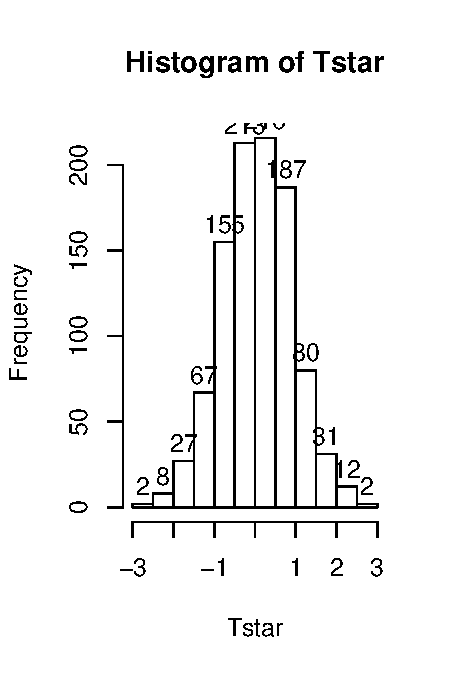
\includegraphics{GreenwoodBanner_files/figure-latex/Figure2-9-1.pdf}
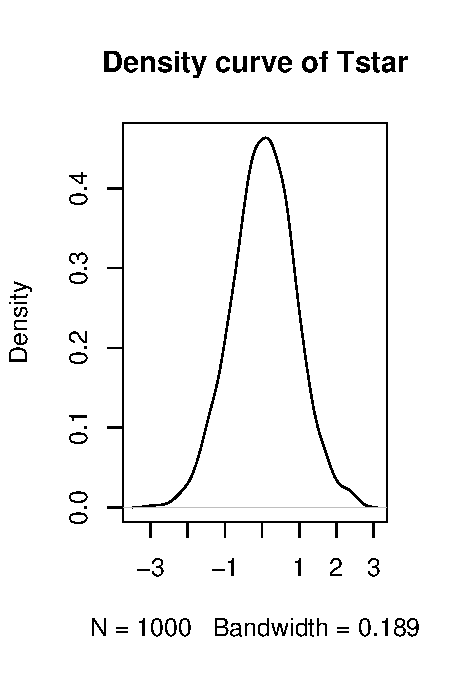
\includegraphics{GreenwoodBanner_files/figure-latex/Figure2-9-2.pdf}

\begin{Shaded}
\begin{Highlighting}[]
\KeywordTok{favstats}\NormalTok{(Tstar)}
\end{Highlighting}
\end{Shaded}

\begin{verbatim}
##        min         Q1     median        Q3      max       mean        sd
##  -2.910384 -0.5099573 0.07681366 0.6102418 2.530583 0.04694168 0.8497364
##     n missing
##  1000       0
\end{verbatim}

Figure \ref{fig:Figure2-9} contains visualizations of \(T^*\) and the
\texttt{favstats} summary provides the related numerical summaries. Our
observed \(T_{obs}\) of 1.84 seems fairly unusual relative to these
results with only 20 \(T^*\) values over 2 based on the histogram. We
need to make more specific comparisons of the permuted results versus
our observed result to be able to clearly decide whether our observed
result is really unusual.

To make the comparisons more concrete, first we can enhance the previous
graphs by adding the value of the test statistic from the real data set,
as shown in Figure \ref{fig:Figure2-10}, using the \texttt{abline}
function.





\begin{Shaded}
\begin{Highlighting}[]
\NormalTok{Tobs <-}\StringTok{ }\FloatTok{1.837}
\KeywordTok{hist}\NormalTok{(Tstar, }\DataTypeTok{labels=}\NormalTok{T)}
\KeywordTok{abline}\NormalTok{(}\DataTypeTok{v=}\NormalTok{Tobs, }\DataTypeTok{lwd=}\DecValTok{2}\NormalTok{, }\DataTypeTok{col=}\StringTok{"red"}\NormalTok{)}
\KeywordTok{plot}\NormalTok{(}\KeywordTok{density}\NormalTok{(Tstar),}\DataTypeTok{main=}\StringTok{"Density curve of Tstar"}\NormalTok{)}
\KeywordTok{abline}\NormalTok{(}\DataTypeTok{v=}\NormalTok{Tobs, }\DataTypeTok{lwd=}\DecValTok{2}\NormalTok{, }\DataTypeTok{col=}\StringTok{"red"}\NormalTok{)}
\end{Highlighting}
\end{Shaded}

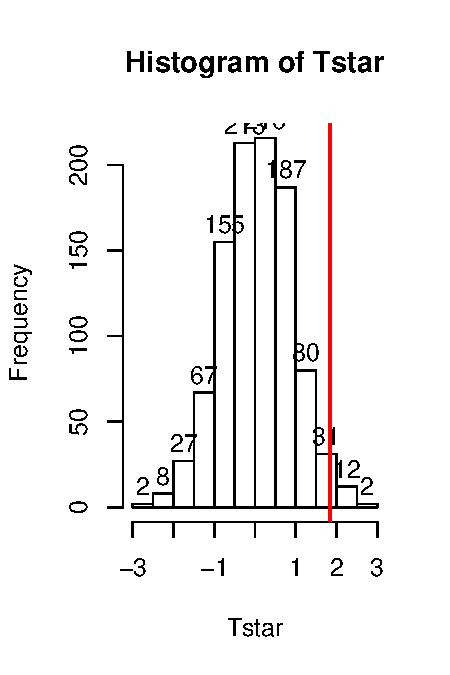
\includegraphics{GreenwoodBanner_files/figure-latex/Figure2-10-1.pdf}
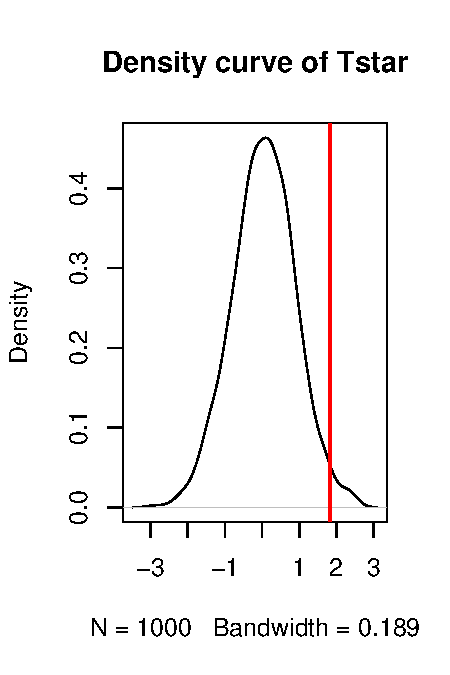
\includegraphics{GreenwoodBanner_files/figure-latex/Figure2-10-2.pdf}

Second, we can calculate the exact number of permuted results that were
larger than what we observed. To calculate the proportion of the 1,000
values that were larger than what we observed, we will use the
\texttt{pdata} function. To use this function, we need to provide the
distribution of values to compare to the cut-off (\texttt{Tstar}), the
cut-off point (\texttt{Tobs}), and whether we want calculate the
proportion that are below (left of) or above (right of) the cut-off
(\texttt{lower.tail=F} option provides the proportion of values above
the cutoff of interest).

\begin{Shaded}
\begin{Highlighting}[]
\KeywordTok{pdata}\NormalTok{(Tstar, Tobs, }\DataTypeTok{lower.tail=}\NormalTok{F)}
\end{Highlighting}
\end{Shaded}

\begin{verbatim}
## [1] 0.02
\end{verbatim}

The proportion of 0.02 tells us that 20 of the 1,000 permuted results
(2\%) were larger than what we observed. This type of work is how we can
generate \textbf{\emph{p-values}} using permutation distributions.
P-values, as you should remember, are the probability of getting a
result as extreme as or more extreme than what we observed, given that
the null is true. Finding only 20 permutations of 1,000 that were larger
than our observed result suggests that it is hard to find a result like
what we observed if there really were no difference, although it is not
impossible.

When testing hypotheses for two groups, there are two types of
alternative hypotheses, one-sided or two-sided. \textbf{\emph{One-sided
tests}} involve only considering differences in one-direction (like
\(\mu_1 > \mu_2\)) and are performed when researchers can decide
\textbf{\emph{a priori}}\footnote{This is a fancy way of saying ``in
  advance'', here in advance of seeing the observations.} which group
should have a larger mean if there is going to be any sort of
difference. In this situation, we did not know enough about the
potential impacts of the pictures to know which group should be larger
than the other so should do a two-sided test. It is important to
remember that you can't look at the responses to decide on the
hypotheses. It is often safer and more
\textbf{\emph{conservative}}\footnote{Statistically, a conservative
  method is one that provides less chance of rejecting the null
  hypothesis in comparison to some other method or less than some
  pre-defined standard.} to start with a \textbf{\emph{two-sided
alternative}} (\(\mathbf{H_A: \mu_1 \ne \mu_2}\)). To do a 2-sided test,
find the area larger than what we observed as above. We also need to add
the area in the other tail (here the left tail) similar to what we
observed in the right tail. Some people suggest doubling the area in one
tail but we will collect information on the number that were more
extreme than the same value in the other tail. In other words, we count
the proportion over 1.84 and below -1.84. So we need to also find how
many of the permuted results were smaller than -1.84years to add to our
previous proportion. Using \texttt{pdata} \texttt{-Tobs} as the cut-off
and \texttt{lower.tail=T} provides this result:

\begin{Shaded}
\begin{Highlighting}[]
\KeywordTok{pdata}\NormalTok{(Tstar, -Tobs, }\DataTypeTok{lower.tail=}\NormalTok{T)}
\end{Highlighting}
\end{Shaded}

\begin{verbatim}
## [1] 0.014
\end{verbatim}

So the p-value to test our null hypothesis of no difference in the true
means between the groups is 0.02 + 0.014, providing a p-value of 0.034.
Figure \ref{fig:Figure2-11} shows both cut-offs on the histogram and
density curve.





\begin{Shaded}
\begin{Highlighting}[]
\KeywordTok{hist}\NormalTok{(Tstar, }\DataTypeTok{labels=}\NormalTok{T)}
\KeywordTok{abline}\NormalTok{(}\DataTypeTok{v=}\KeywordTok{c}\NormalTok{(-}\DecValTok{1}\NormalTok{,}\DecValTok{1}\NormalTok{)*Tobs, }\DataTypeTok{lwd=}\DecValTok{2}\NormalTok{, }\DataTypeTok{col=}\StringTok{"red"}\NormalTok{)}
\KeywordTok{plot}\NormalTok{(}\KeywordTok{density}\NormalTok{(Tstar),}\DataTypeTok{main=}\StringTok{"Density curve of Tstar"}\NormalTok{)}
\KeywordTok{abline}\NormalTok{(}\DataTypeTok{v=}\KeywordTok{c}\NormalTok{(-}\DecValTok{1}\NormalTok{,}\DecValTok{1}\NormalTok{)*Tobs, }\DataTypeTok{lwd=}\DecValTok{2}\NormalTok{, }\DataTypeTok{col=}\StringTok{"red"}\NormalTok{)}
\end{Highlighting}
\end{Shaded}

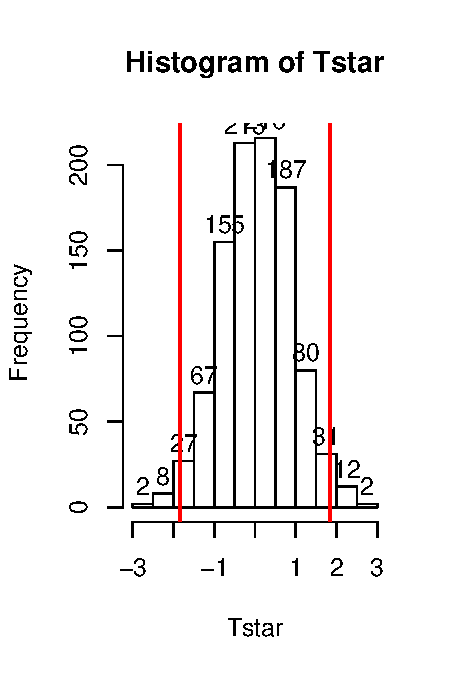
\includegraphics{GreenwoodBanner_files/figure-latex/Figure2-11-1.pdf}
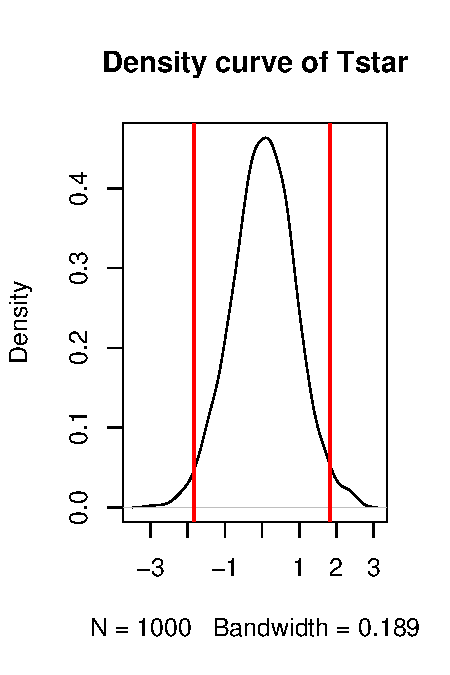
\includegraphics{GreenwoodBanner_files/figure-latex/Figure2-11-2.pdf}

In general, the \textbf{\emph{one-sided test p-value}} is the proportion
of the permuted results that are more extreme than observed in the
direction of the \emph{alternative} hypothesis (lower or upper tail,
remembering that this also depends on the direction of the difference
taken). For the 2-sided test, the p-value is the proportion of the
permuted results that are \emph{less than the negative version of the
observed statistic and greater than the positive version of the observed
statistic}. Using absolute values (\textbar{} \textbar{}), we can
simplify this: the \textbf{\emph{two-sided p-value}} is the
\emph{proportion of the \textbar{}permuted statistics\textbar{} that are
larger than \textbar{}observed statistic\textbar{}}. This will always
work and finds areas in both tails regardless of whether the observed
statistic is positive or negative. In R, the \texttt{abs} function
provides the \textbf{\emph{absolute value}} and we can again use
\texttt{pdata} to find our p-value in one line of code:

\begin{Shaded}
\begin{Highlighting}[]
\KeywordTok{pdata}\NormalTok{(}\KeywordTok{abs}\NormalTok{(Tstar), }\KeywordTok{abs}\NormalTok{(Tobs), }\DataTypeTok{lower.tail=}\NormalTok{F)}
\end{Highlighting}
\end{Shaded}

\begin{verbatim}
## [1] 0.034
\end{verbatim}

We will discuss the choice of \textbf{\emph{significance level}} below,
but for the moment, assume that \(\alpha\) is chosen to be our standard
value of 0.05. Since the p-value is smaller than \(\alpha\), this
suggests that we can \textbf{\emph{reject the null hypothesis}} and
conclude that there is evidence of some difference in the true mean
sentences given between the two types of pictures.

Before we move on, let's note some interesting features of the
permutation distribution of the difference in the sample means shown in
Figure \ref{fig:Figure2-11}.

\begin{enumerate}
\def\labelenumi{\arabic{enumi}.}
\item
  It is basically centered at 0. Since we are performing permutations
  assuming the null model is true, we are assuming that
  \(\mu_1 = \mu_2\) which implies that \(\mu_1 - \mu_2 = 0\). This also
  suggests that 0 should be the center of the permutation distribution
  and it was.
\item
  It is approximately normally distributed. This is due to the
  \textbf{\emph{Central Limit Theorem}}\footnote{We'll leave the
    discussion of the CLT to your previous stat coursework or an
    internet search. Remember that it has something to do with
    distributions looking more normal as the sample size increases.},
  where the\\
  \textbf{\emph{sampling distribution}} (distribution of all possible
  results for samples of this size) of the difference in sample means
  (\(\bar{x}_1 - \bar{x}_2\)) becomes more and normally distributed as
  the sample sizes increase. With 38 and 37 observations in the groups,
  we are likely to have a relatively normal looking distribution of the
  difference in the sample means. This result will allow us to use a
  parametric method to approximate this sampling distribution under the
  null model if some assumptions are met, as we'll discuss below.
\item
  Our observed difference in the sample means (1.84 years) is a fairly
  unusual result relative to the rest of these results but there are
  some permuted data sets that produce more extreme differences in the
  sample means. When the observed differences are really large, we may
  not see any permuted results that are as extreme as what we observed.
  When \texttt{pdata} gives you 0, the p-value should be reported to be
  smaller than 0.0001 (\textbf{not 0!}) since it happened in less than 1
  in 1000 tries but does occur once -- in the actual dataset.
\item
  Since our null model is not specific about the direction of the
  difference, considering a result like ours but in the other direction
  (-1.84 years) needs to be included. The observed result seems to put
  about the same area in both tails of the distribution but it is not
  exactly the same. The small difference in the tails is a useful aspect
  of this approach compared to the parametric method discussed below as
  it accounts for slight asymmetry in the sampling distribution.
\end{enumerate}

Earlier, we decided that the p-value was small enough to reject the null
hypothesis since it was smaller than our chosen level of significance.
In this course, you will often be allowed to use your own judgment about
an appropriate significance level in a particular situation (in other
words, if we forget to tell you an \(\alpha\) -level, you can still make
a decision using a reasonably selected significance level). Remembering
that the p-value is the probability you would observe a result like you
did (or more extreme), assuming the null hypothesis is true, this tells
you that the smaller the p-value is, the more evidence you have against
the null. The next section provides a more formal review of the
hypothesis testing infrastructure, terminology, and some of things that
can happen when testing hypotheses.

\section{Hypothesis testing (general)}\label{section2-5}

In hypothesis testing, it is formulated to answer a specific question
about a population or true parameter(s) using a statistic based on a
data set. In your previous statistics course, you (hopefully) considered
one-sample hypotheses about population means and proportions and the two
sample mean situation we are focused on here. Our hypotheses relate to
trying to answer the question about whether the population mean
sentences between the two groups are different, with an initial
assumption of no difference.

Hypothesis testing is much like a criminal trial where you are in the
role of a jury member or judge, if no jury is present. Initially, the
defendant is assumed innocent. In our situation, the true means are
assumed to be equal between the groups. Then evidence is presented and,
as a juror, you analyze it. In statistical hypothesis testing, data are
collected and analyzed. Then you have to decide if we had ``enough''
evidence to reject the initial assumption (``innocence'' that is
initially assumed). To make this decision, you want to have previously
decided on the standard of evidence required to reject the initial
assumption. In criminal cases, ``beyond a reasonable doubt'' is used.
Wikipedia's definition
(\url{https://en.wikipedia.org/wiki/Reasonable_doubt}) suggests that
this standard is that ``there can still be a doubt, but only to the
extent that it would not affect a reasonable person's belief regarding
whether or not the defendant is guilty''. In civil trials, a lower
standard called a ``preponderance of evidence'' is used. Based on that
defined and pre-decided (\emph{a priori}) measure, you decide that the
defendant is guilty or not guilty. In statistics, we compare our p-value
to a significance level, \(\alpha\), which is most of the time selected
to be 5\%. If our p-value is less than \(\alpha\), we reject the null
hypothesis. The choice of the significance level is like the variation
in standards of evidence between criminal and civil trials -- and in all
situations everyone should know the standards required for rejecting the
initial assumption before any information is ``analyzed''. Once someone
is found guilty, then there is the matter of sentencing which is related
to the impacts (``size'') of the crime. In statistics, this is similar
to the estimated size of differences and the related judgments about
whether the differences are practically important or not. If the crime
is proven beyond a reasonable doubt but it is a minor crime, then the
sentence will be small. With the same level of evidence and a more
serious crime, the sentence will be more dramatic.

There are some important aspects of the testing process to note that
inform how we interpret statistical hypothesis test results. When
someone is found ``not guilty'', it does not mean ``innocent'', it just
means that there was not enough evidence to find the person guilty
``beyond a reasonable doubt''. Not finding enough evidence to reject the
null hypothesis does not imply that the true means are equal, just that
there was not enough evidence to conclude that they were different.
There are many potential reasons why we might fail to reject the null,
but the most common one is that our sample size was too small (which is
related to having too little evidence).

Throughout this material, we will continue to re-iterate the
distinctions between parameters and statistics and want you to be clear
about the distinctions between estimates based on the sample and
inferences for the population or true values of the parameters of
interest. Remember that statistics are summaries of the sample
information and parameters are characteristics of populations (which we
rarely know). In the two-sample mean situation, the sample means are
always at least a little different -- that is not an interesting
conclusion. What is interesting is whether we have enough evidence to
prove that the population or true means differ ``beyond a reasonable
doubt''.

The scope of any inferences is constrained based on whether there is a\\
\textbf{\emph{random sample}} (RS) and/or \textbf{\emph{random
assignment}} (RA). Table \ref{tab:Table2-1} contains the four possible
combinations of these two characteristics of a given study. Random
assignment allows for causal inferences for differences that are
observed -- the difference in treatment levels causes differences in the
mean responses. Random sampling (or at least some sort of representative
sample) allows inferences to be made to the population of interest. If
we do not have RA, then causal inferences cannot be made. If we do not
have a representative sample, then our inferences are limited to the
sampled subjects.



\begin{table}

\caption{\label{tab:Table2-1}Scope of inference summary.}
\centering
\begin{tabular}[t]{l|l|l}
\hline
**Random Sampling/Random Assignment** & **Random Assignment (RA) -- Yes (controlled experiment)** & **Random Assignment (RA) -- No (observational study)**\\
\hline
**Random Sampling (RS) -- Yes (or some method that results in a representative sample of population of interest)** & Because we have RS, we can generalize inferences to the population the RS was taken from. Because we have RA we can assume the groups were equivalent on all aspects except for the treatment and can establish causal inference. & Can generalize inference to population the RS was taken from but cannot establish causal inference (no RA - cannot isolate treatment variable as only difference among groups, could be confounding variables).\\
\hline
**Random Sampling (RS) -- No (usually a convenience sample)** & Cannot generalize inference to the population of interest because the sample was not random and could be biased - may not be "representative" of the population of interest. Can establish causal inference due to RA   \&rarr; the inference from this type of study applies only to the sample. & Cannot generalize inference to the population of interest because the sample was not random and could be biased - may not be "representative" of the population of interest. Cannot establish causal inference due to lack of RA of the treatment.\\
\hline
\end{tabular}
\end{table}

A simple example helps to clarify how the scope of inference can change.
Suppose we are interested in studying the GPA of students. If we had
taken a random sample from, say, the STAT 217 students in a given
semester, our scope of inference would be the population of 217 students
in that semester. If we had taken a random sample from the entire MSU
population, then the inferences would be to the entire MSU population in
that semester. These are similar types of problems but the two
populations are very different and the group you are trying to make
conclusions about should be noted carefully in your results -- it does
matter! If we did not have a representative sample, say the students
could choose to provide this information or not, then we can only make
inferences to volunteers. These volunteers might differ in systematic
ways from the entire population of STAT 217 students so we cannot safely
extend our inferences beyond the group that volunteered.

To consider the impacts of RA versus observational studies, we need to
be comparing groups. Suppose that we are interested in differences in
the mean GPAs for different sections of STAT 217 and that we take a
random sample of students from each section and compare the results and
find evidence of some difference. In this scenario, we can conclude that
there is some difference in the population of STAT 217 students but we
can't say that being in different sections caused the differences in the
mean GPAs. Now suppose that we randomly assigned every 217 student to
get extra training in one of three different study techniques and found
evidence of differences among the training methods. We could conclude
that the training methods caused the differences in these students.
These conclusions would only apply to STAT 217 students and could not be
generalized to a larger population of students. If we took a random
sample of STAT 217 students (say only 10 from each section) and then
randomly assigned them to one of three training programs and found
evidence of differences, then we can say that the training programs
caused the differences. We can also say that we have evidence that those
differences pertain to the population of STAT 217 students. This seems
similar to the scenario where all 217 students participated in the
training programs except that by using random sampling, only a fraction
of the population needs to actually be studied to make inferences to the
entire population of interest -- saving time and money.

A quick summary of the terminology of hypothesis testing is useful at
this point. The \textbf{\emph{null hypothesis}} (\(H_0\)) states that
there is no difference or no relationship in the population. This is the
statement of no effect or no difference and the claim that we are trying
to find evidence against. In this chapter, \(H_0\): \(\mu_1=\mu_2\).
When doing two-group problems, you always need to specify which group is
1 and which one is 2 because the order does matter. The
\textbf{\emph{alternative hypothesis}} (\(H_1\) or \(H_A\)) states a
specific difference between parameters. This is the research hypothesis
and the claim about the population that we hope to demonstrate is more
reasonable to conclude than the null hypothesis. In the two-group
situation, we can have \textbf{\emph{one-sided alternatives}}
\(H_A\):\(\mu_1 > \mu_2\) (greater than) or \(H_A\):\(\mu_1 < \mu_2\)
(less than) or, the more common, \textbf{\emph{two-sided alternative}}
\(H_A\):\(\mu_1 \ne \mu_2\) (not equal to). We usually default to using
two-sided tests because we often do not know enough to know the
direction of a difference in advance, especially in more complicated
situations. The \textbf{\emph{sampling distribution under the null}} is
the distribution of all possible values of a statistic under \(H_0\) is
true. It is used to calculate the \textbf{\emph{p-value}} , the
probability of obtaining a result as extreme or more extreme than what
we observed given that the null hypothesis is true. We will find
sampling distributions using\\
\textbf{\emph{nonparametric}} approaches (like the permutation approach
used above) and \textbf{\emph{parametric}} methods (using ``named''
distributions like the \(t\), F, and \(\chi^2\)).

Small p-values are evidence against the null hypothesis because the
observed result is unlikely due to chance if \(H_0\) is true. Large
p-values provide no evidence against \(H_0\) but do not allow us to
conclude that there is no difference. The \textbf{\emph{level of
significance}} is an \emph{a priori} definition of how small the p-value
needs to be to provide ``enough'' (sufficient) evidence against \(H_0\).
This is most useful to prevent sliding the standards after the results
are found. We compare the p-value to the level of significance to decide
if the p-value is small enough to constitute sufficient evidence to
reject the null hypothesis. We use \(\alpha\) to denote the level of
significance and most typically use 0.05 which we refer to as the 5\%
significance level. We compare the p-value to this level and make a
decision. The two options for \emph{decisions} are to either
\emph{reject the null hypothesis} if the p-value \(\le \alpha\) or
\emph{fail to reject the null hypothesis} if the p-value \(> \alpha\).
When interpreting hypothesis testing results, remember that the p-value
is a measure of how unlikely the observed outcome was, assuming that the
null hypothesis is true. It is \textbf{NOT} the probability of the data
or the probability of either hypothesis being true. The p-value, simply,
is a measure of evidence against the null hypothesis.

The specific definition of \(\alpha\) is that it is the probability of
rejecting \(H_0\) when \(H_0\) is true, the probability of what is
called a \textbf{\emph{Type I error}}. Type I errors are also called
\textbf{\emph{false rejections}}. In the two-group mean situation, a
Type I error would be concluding that there is a difference in the true
means between the groups when none really exists in the population. In
the courtroom setting, this is like falsely finding someone guilty. We
don't want to do this very often, so we use small values of the
significance level, allowing us to control the rate of Type I errors at
\(\alpha\). We also have to worry about \textbf{Type II errors}, which
are failing to reject the null hypothesis when it's false. In a
courtroom, this is the same as failing to convict a truley guilty
person. This most often occurs due to a lack of evidence. You can use
the Table \ref{tab:Table2-2} to help you remember all the possibilities.




\begin{table}

\caption{\label{tab:Table2-2}Table of decisions and truth scenarios in a hypothesis
testing situation. But we never know the truth in a real situation.}
\centering
\begin{tabular}[t]{l|l|l}
\hline
 & **H<sub>0</sub> True** & **H<sub>0</sub> False**\\
\hline
**FTR H<sub>0</sub>** & Correct decision & Type II error\\
\hline
**Reject H<sub>0</sub>** & Type I error & Correct decision\\
\hline
\end{tabular}
\end{table}

In comparing different procedures, there is an interest in studying the
rate or probability of Type I and II errors. The probability of a Type I
error was defined previously as \(\alpha\), the significance level. The
\textbf{\emph{power}} of a procedure is the probability of rejecting the
null hypothesis when it is false. Power is defined as

\[\text{Power} = 1 - \text{Probability(Type II error) } = 
\text{Probability(Reject) } H_0 | H_0 \text{ is false),}\]

or, in words, the probability of detecting a difference when it actually
exists. We want to use a statistical procedure that controls the Type I
error rate at the pre-specified level and has high power to detect false
null alternatives. Increasing the sample size is one of the most
commonly used methods for increasing the power in a given situation.
Sometimes we can choose among different procedures and use the power of
the procedures to help us make that selection. Note that there are many
ways \(H_0\) false and the power changes based on how false the null
hypothesis actually is. To make this concrete, suppose that the true
mean sentences differed by either 1 or 20 years in previous example. The
chances of rejecting the null hypothesis are much larger when the groups
actually differ by 20 years than if they differ by just 1 year.

After making a decision (was there enough evidence to reject the null or
not), we want to make the conclusions specific to the problem of
interest. If we reject \(H_0\), then we can conclude that there was
sufficient evidence at the \(\alpha\)-level that the null hypothesis is
wrong (and the results point in the direction of the alternative). If we
fail to reject \(H_0\) (FTR \(H_0\)), then we can conclude that there
was insufficient evidence at the \(\alpha\)-level to say that the null
hypothesis is wrong. We are \textbf{NOT} saying that the null is correct
and we \textbf{NEVER} accept the null hypothesis. We just failed to find
enough evidence to say it's wrong. If we find sufficient evidence to
reject the null, then we need to revisit the method of data collection
and design of the study to discuss scope of inference. Can we discuss
causality (due to RA) and/or make inferences to a larger group than
those in the sample (due to RS)?

To perform a hypothesis test, there are some steps to remember to
complete to make sure you have thought through all the aspects of the
results.

\begin{longtable}[]{@{}l@{}}
\toprule
\begin{minipage}[t]{0.97\columnwidth}\raggedright\strut
\textbf{Outline of 6+ steps to perform a Hypothesis Test}\strut
\end{minipage}\tabularnewline
\begin{minipage}[t]{0.97\columnwidth}\raggedright\strut
Isolate the claim to be proved, method to use (define a test statistic
T), and significance level.\strut
\end{minipage}\tabularnewline
\begin{minipage}[t]{0.97\columnwidth}\raggedright\strut
1. Write the null and alternative hypotheses,\strut
\end{minipage}\tabularnewline
\begin{minipage}[t]{0.97\columnwidth}\raggedright\strut
2. Assess the ``Validity Conditions'' for the procedure being used
(discussed below),\strut
\end{minipage}\tabularnewline
\begin{minipage}[t]{0.97\columnwidth}\raggedright\strut
3. Find the value of the appropriate test statistic,\strut
\end{minipage}\tabularnewline
\begin{minipage}[t]{0.97\columnwidth}\raggedright\strut
4. Find the p-value,\strut
\end{minipage}\tabularnewline
\begin{minipage}[t]{0.97\columnwidth}\raggedright\strut
5. Make a decision, and\strut
\end{minipage}\tabularnewline
\begin{minipage}[t]{0.97\columnwidth}\raggedright\strut
6. Write a conclusion specific to the problem, including scope of
inference discussion.\strut
\end{minipage}\tabularnewline
\bottomrule
\end{longtable}

\section{Connecting randomization (nonparametric) and parametric
tests}\label{section2-6}

In developing statistical inference techniques, we need to define the
test quantity of interest. To compare the means of two groups, a
statistic is needed that measures their differences. In general, for
comparing two groups, the choices are simple -- a difference in the
means often works well and is a natural choice. There are other options
such as tracking the ratio of means or possibly the difference in
medians. Instead of just using the difference in the means, we also
could ``standardize'' the difference in the means by dividing by an
appropriate quantity that reflects the variation in the difference in
the means. All of these are valid and can sometimes provide similar
results - it ends up that there are many possibilities for testing using
the randomization (nonparametric) techniques introduced previously.
Parametric statistical methods focus on means because the statistical
theory surrounding means is quite a bit easier (not easy, just easier)
than other options but there are just a couple of test statistics that
you can use and end up with named distributions to use for generating
inferences. Randomization techniques allow inference for other
quantities but our focus here will be on using randomization for
inferences on means to see the similarities with the more traditional
parametric procedures.

In two-sample mean situations, instead of working just with the
difference in the means, we often calculate a test statistic that is
called the\\
\textbf{\emph{equal variance two-independent samples t-statistic}}. The
test statistic is

\[t = \frac{\bar{x}_1 - \bar{x}_2}{s_p\sqrt{\frac{1}{n_1}+\frac{1}{n_2}}},\]

where \(s_1^2\) and \(s_2^2\) are the sample variances for the two
groups, \(n_1\) and \(n_2\) are the sample sizes for the two groups, and
the \textbf{\emph{pooled sample standard deviation}} ,

\[s_p = \sqrt{\frac{(n_1-1)s_1^2 + (n_2-1)s_2^2}{n_1+n_2-2}}.\]

The \(t\)-statistic keeps the important comparison between the means in
the numerator that we used before and standardizes (re-scales) that
difference so that \(t\) will follow a \(t\)-distribution (a parametric
``named''distribution) if certain assumptions are met. But first we
should see if standardizing the difference in the means had an impact on
our permutation test results. Instead of using the \texttt{diffmean}
function, we will use the \texttt{t.test} function (see its full use
below) and have it calculate the formula for \(t\) for us. The R code
``\texttt{\$statistic}'' is basically a way of extracting just the
number we want to use for \(T\) from a larger set of output the
\texttt{t.test} function wants to provide you. We will see below that
\texttt{t.test} switches the order of the difference (now it is
\emph{Average} - \emph{Unattractive}) -- always carefully check for the
direction of the difference in the results. Since we are doing a
two-sided test, the code resembles the permutation test code in Section
\ref{section2-4} with the new \(t\)-statistic replacing the difference
in the sample means that we used before.

The permutation distribution in Figure \ref{fig:Figure2-12} looks
similar to the previous results with slightly different \(x\)-axis
scaling. The the proportion of permuted results that were more extreme
than the observed result was 0.031. This difference is due to a
different set of random permutations being selected. If you run
permutation code, you will often get slightly different results each
time you run it. If you are uncomfortable with the variation in the
results, you can run more than \(B=\) 1,000 permutations (say 10,000)
and the variability in the resulting p-values will be reduced further.
Usually this uncertainty will not cause any substantive problems -- but
do not be surprised if your results vary from a colleagues if you are
both analyzing the same data set or if you re-run your permutation code.



\begin{Shaded}
\begin{Highlighting}[]
\NormalTok{Tobs <-}\StringTok{ }\KeywordTok{t.test}\NormalTok{(Years ~}\StringTok{ }\NormalTok{Attr, }\DataTypeTok{data=}\NormalTok{MockJury2, }\DataTypeTok{var.equal=}\NormalTok{T)$statistic}
\NormalTok{Tobs}
\end{Highlighting}
\end{Shaded}

\begin{verbatim}
##        t 
## -2.17023
\end{verbatim}

\begin{Shaded}
\begin{Highlighting}[]
\NormalTok{Tstar <-}\StringTok{ }\KeywordTok{matrix}\NormalTok{(}\OtherTok{NA}\NormalTok{, }\DataTypeTok{nrow=}\NormalTok{B)}
\NormalTok{for (b in (}\DecValTok{1}\NormalTok{:B))\{}
  \NormalTok{Tstar[b] <-}\StringTok{ }\KeywordTok{t.test}\NormalTok{(Years ~}\StringTok{ }\KeywordTok{shuffle}\NormalTok{(Attr), }\DataTypeTok{data=}\NormalTok{MockJury2, }\DataTypeTok{var.equal=}\NormalTok{T)$statistic}
\NormalTok{\}}
\KeywordTok{hist}\NormalTok{(Tstar, }\DataTypeTok{labels=}\NormalTok{T)}
\KeywordTok{abline}\NormalTok{(}\DataTypeTok{v=}\KeywordTok{c}\NormalTok{(-}\DecValTok{1}\NormalTok{,}\DecValTok{1}\NormalTok{)*Tobs, }\DataTypeTok{lwd=}\DecValTok{2}\NormalTok{, }\DataTypeTok{col=}\StringTok{"red"}\NormalTok{)}
\KeywordTok{plot}\NormalTok{(}\KeywordTok{density}\NormalTok{(Tstar), }\DataTypeTok{main=}\StringTok{"Density curve of Tstar"}\NormalTok{)}
\KeywordTok{abline}\NormalTok{(}\DataTypeTok{v=}\KeywordTok{c}\NormalTok{(-}\DecValTok{1}\NormalTok{,}\DecValTok{1}\NormalTok{)*Tobs, }\DataTypeTok{lwd=}\DecValTok{2}\NormalTok{, }\DataTypeTok{col=}\StringTok{"red"}\NormalTok{)}
\KeywordTok{pdata}\NormalTok{(}\KeywordTok{abs}\NormalTok{(Tstar),}\KeywordTok{abs}\NormalTok{(Tobs),}\DataTypeTok{lower.tail=}\NormalTok{F)}
\end{Highlighting}
\end{Shaded}

\begin{verbatim}
##     t 
## 0.031
\end{verbatim}

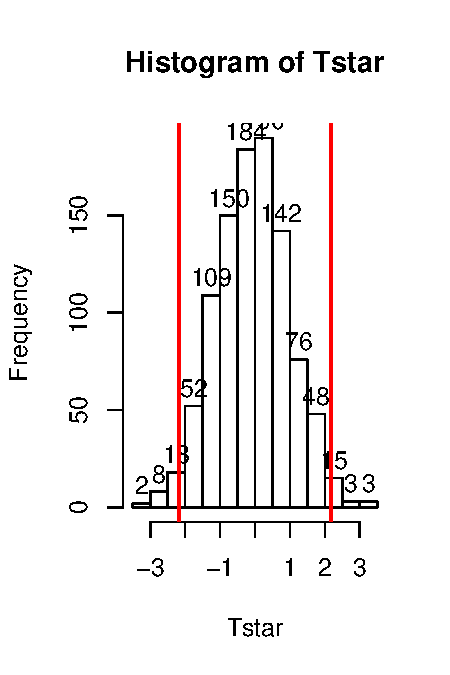
\includegraphics{GreenwoodBanner_files/figure-latex/Figure2-12-1.pdf}
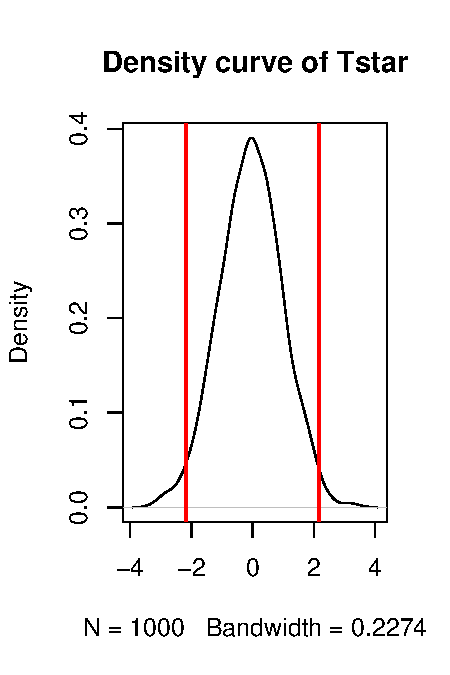
\includegraphics{GreenwoodBanner_files/figure-latex/Figure2-12-2.pdf}

The parametric version of these results is based on using what is called
the \textbf{\emph{two-independent sample t-test}}. There are actually
two versions of this test, one that assumes that variances are equal in
the groups and one that does not. There is a rule of thumb that if the
\textbf{ratio of the larger standard deviation over the smaller standard
deviation is less than 2, the equal variance procedure is ok}. It ends
up that this assumption is less important if the sample sizes in the
groups are approximately equal and more important if the groups contain
different numbers of observations. In comparing the two potential test
statistics, the procedure that assumes equal variances has a complicated
denominator (see the formula above for \(t\) involving \(s_p\)) but a
simple formula for \textbf{\emph{degrees of freedom}}
(\textbf{\emph{df}}) for the \(t\)-distribution (\(df=n_1+n_2-2\)) that
approximates the distribution of the test statistic, \(t\), under the
null hypothesis. The procedure that assumes unequal variances has a
simpler test statistic and a very complicated degrees of freedom
formula. The equal variance procedure is most similar to the ANOVA
methods we will consider in Chapters 2 and 3 so that will be our focus
for the two group problem. Fortunately, both of these methods are
readily available in the \texttt{t.test} function in R if needed.

If the assumptions for the equal variance \(t\)-test are met and the
null hypothesis is true, then the sampling distribution of the test
statistic should follow a \(t\)-distribution with \(n_1+n_2-2\) degrees
of freedom. The \textbf{\emph{t-distribution}} is a bell-shaped curve
that is more spread out for smaller values of degrees of freedom as
shown in Figure \ref{fig:Figure2-13}. The \(t\)-distribution looks more
and more like a \textbf{\emph{standard normal distribution}}
(\(N(0,1)\)) as the degrees of freedom increase.



\begin{figure}
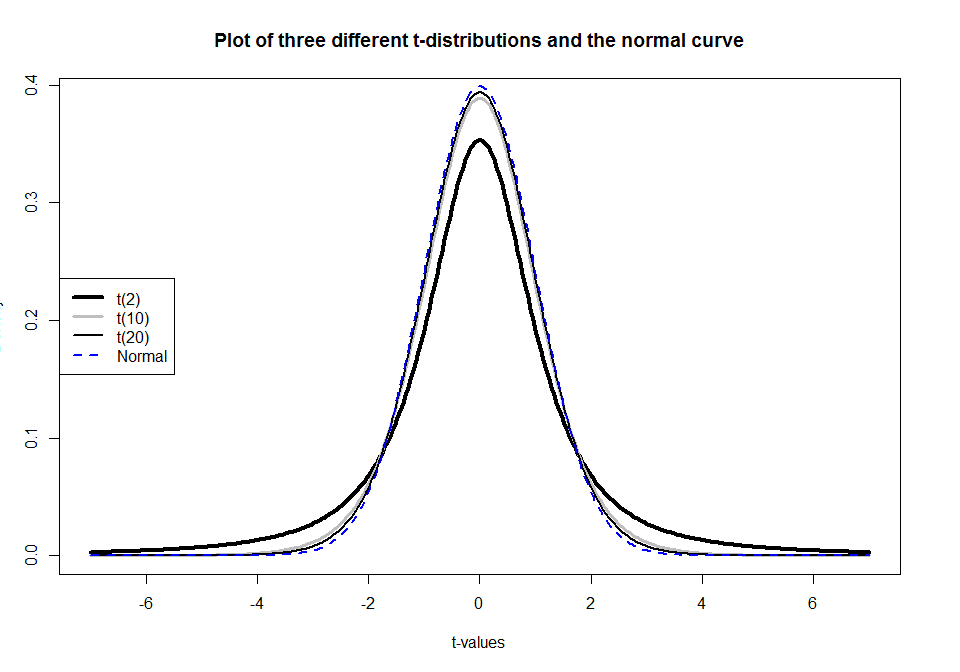
\includegraphics[width=13.33in]{chapter1_files/image045} \caption{Plots of \(t\) and normal distributions}\label{fig:Figure2-13}
\end{figure}

To get the p-value for the parametric \(t\)-test, we need to calculate
the test statistic and \(df\), then look up the areas in the tails of
the \(t\)-distribution relative to the observed \(t\)-statistic. We'll
learn how to use R to do this below, but for now we will allow the
\texttt{t.test} function to take care of this for us. The
\texttt{t.test} function uses our formula notation
(\texttt{Years\ \textasciitilde{}\ Attr}) and then \texttt{data=...} as
we saw before for making plots. To get the equal-variance test result,
the \texttt{var.equal=T} option needs to be turned on. Then
\texttt{t.test} provides us with lots of useful output. The three
results we've been discussing are highlighted in the output below -- the
test statistic value (-2.17), \(df=73\), and the p-value, from the
\(t\)-distribution with 73 degrees of freedom, of 0.033.

\begin{Shaded}
\begin{Highlighting}[]
\KeywordTok{t.test}\NormalTok{(Years ~}\StringTok{ }\NormalTok{Attr, }\DataTypeTok{data=}\NormalTok{MockJury2, }\DataTypeTok{var.equal=}\NormalTok{T)}
\end{Highlighting}
\end{Shaded}

\begin{verbatim}
## 
##  Two Sample t-test
## 
## data:  Years by Attr
## t = -2.1702, df = 73, p-value = 0.03324
## alternative hypothesis: true difference in means is not equal to 0
## 95 percent confidence interval:
##  -3.5242237 -0.1500295
## sample estimates:
##      mean in group Average mean in group Unattractive 
##                   3.973684                   5.810811
\end{verbatim}

So the parametric \(t\)-test gives a p-value of 0.033 from a test
statistic of -2.1702. The negative sign on the test statistic occurred
because the function took \emph{Average} - \emph{Unattractive} which is
the opposite direction as \texttt{diffmean}. The p-value is very similar
to the two permutation results found before. The reason for this
similarity is that the permutation distribution with 73 degrees of
freedom. Figure \ref{fig:Figure2-14} shows how similar the two
distributions happened to be here.



\begin{figure}
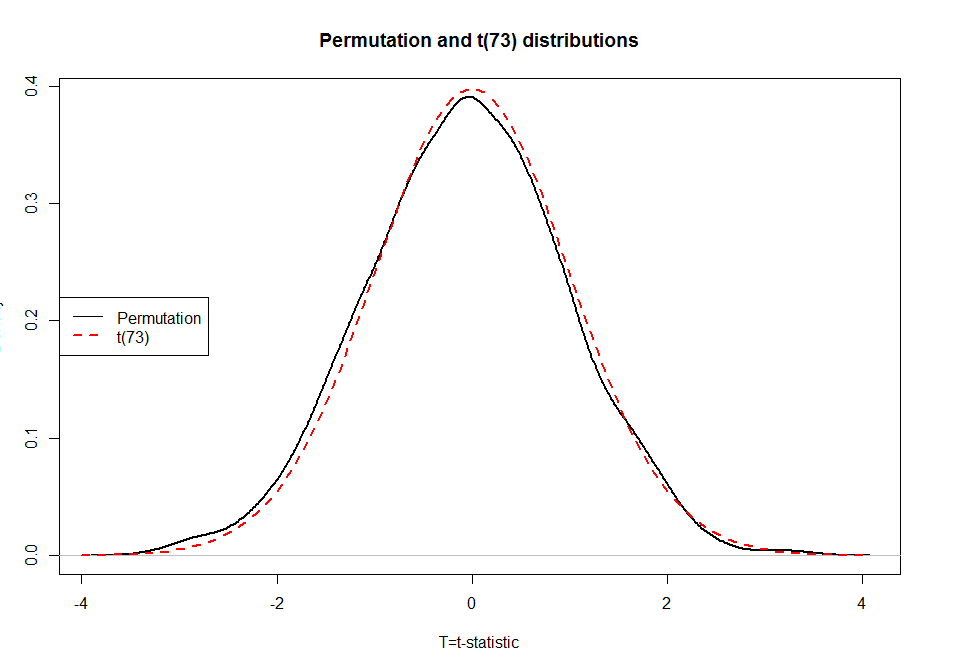
\includegraphics[width=13.33in]{chapter1_files/image047} \caption{Plot of permutation and \(t\) distribution with \(df=73\).}\label{fig:Figure2-14}
\end{figure}

In your previous statistics course, you might have used an applet or a
table to find p-values such as what was provided in the previous R
output. When not directly provided in the output of a function, R can be
used to look up p-values\footnote{On exams, you will be asked to
  describe the area of interest, sketch a picture of the area of
  interest, and/or note the distribution you would use.} from named
distributions such as the \(t\)-distribution. In this case, the
distribution of the test statistic under the null hypothesis is a
\(t(73)\) or a \(t\) with 73 degrees of freedom. The \texttt{pt}
function is used to get p-values from the \(t\)-distribution in the same
manner that \texttt{pdata} could help us to find p-values from the
permutation distribution. We need to provide the \texttt{df=...} and
specify the tail of the distribution of interest using the
\texttt{lower.tail} option along with the cutoff of interest. If we want
the area to the left of -2.17:

\begin{Shaded}
\begin{Highlighting}[]
\KeywordTok{pt}\NormalTok{(-}\FloatTok{2.1702}\NormalTok{, }\DataTypeTok{df=}\DecValTok{73}\NormalTok{, }\DataTypeTok{lower.tail=}\NormalTok{T)}
\end{Highlighting}
\end{Shaded}

\begin{verbatim}
## [1] 0.01662286
\end{verbatim}

And we can double it to get the p-value that \texttt{t.test} provided
earlier, because the \(t\)-distribution is symmetric:

\begin{Shaded}
\begin{Highlighting}[]
\DecValTok{2}\NormalTok{*}\KeywordTok{pt}\NormalTok{(-}\FloatTok{2.1702}\NormalTok{, }\DataTypeTok{df=}\DecValTok{73}\NormalTok{, }\DataTypeTok{lower.tail=}\NormalTok{T)}
\end{Highlighting}
\end{Shaded}

\begin{verbatim}
## [1] 0.03324571
\end{verbatim}

More generally, we could always make the test statistic positive using
the absolute value, find the area to the right of it, and then double
that for a two-sided test p-value:

\begin{Shaded}
\begin{Highlighting}[]
\DecValTok{2}\NormalTok{*}\KeywordTok{pt}\NormalTok{(}\KeywordTok{abs}\NormalTok{(-}\FloatTok{2.1702}\NormalTok{), }\DataTypeTok{df=}\DecValTok{73}\NormalTok{, }\DataTypeTok{lower.tail=}\NormalTok{T)}
\end{Highlighting}
\end{Shaded}

\begin{verbatim}
## [1] 1.966754
\end{verbatim}

Permutation distributions do not need to match the named parametric
distribution to work correctly, although this happened in the previous
example. The parametric certain conditions to be met for the sampling
distribution of the statistic to follow the named distribution and
provide accurate p-values. The conditions for the equal variance t-test
are:

\begin{enumerate}
\def\labelenumi{\arabic{enumi}.}
\item
  \textbf{Independent observations}: Each observation obtained is
  unrelated to all other observations. To assess this, consider whether
  anything in the data collection might lead to clustered or related
  observations that are un-related to the differences in the groups. For
  example, was the same person measured more than once?\footnote{In some
    studies, the same subject might be measured in both conditions and
    this violates the assumptions of this procedure.}
\item
  \textbf{Equal variances} in the groups (because we used a procedure
  that assumes equal variances! -- there is another procedure that
  allows you to relax this assumption if needed\ldots{}). To assess
  this, compare the standard deviations and variability in the beanplots
  and see if they look noticeably different. Be particularly critical of
  this assessment if the sample sizes differ greatly between groups.
\item
  \textbf{Normal distributions} of the observations in each group. We'll
  learn more diagnostics later, but the boxplots and beanplots are a
  good place to start to help you look for skews or outliers, which were
  both present here. If you find skew and/or outliers, that would
  suggest a problem with the assumption of normality as normal
  distributions are symmetric and extreme observations occur very
  rarely.
\end{enumerate}

For the permutation test, we relax the third condition and replace it
with:

\begin{enumerate}
\def\labelenumi{\arabic{enumi}.}
\setcounter{enumi}{2}
\tightlist
\item
  \textbf{\emph{Similar distributions between the groups:}} The
  permutation approach allows valid inferences as long as the two groups
  have similar shapes and only possibly differ in their centers. In
  other words, the distributions need not look normal for the procedure
  to work well, but they do need to look similar.
\end{enumerate}

In the prisoner ``juror'' study, we can assume that the independent
observation condition is met because there is no information suggesting
that the same subjects were measured more than once or that some other
type of grouping in the responses was present (like the subjects were
divided in groups and placed in rooms to discuss their responses prior
to submitting them). The equal variance condition might be violated. The
variances need not be equal as the procedure can still provide
reasonable results with some violation of this assumption. The standard
deviations are 2.8 vs 4.4, so this difference is not ``large'' according
to the rule of thumb noted above. It is, however, close to being
considered problematic. It would be difficult to reasonably assume that
the normality condition is met here (Figure \ref{fig:Figure2-6} with
clear right skews in both groups and potential outliers which causes
concerns for (3) for the parametric procedure. The shapes look similar
for the two groups so there is less reason to be concerned with using
the permutation approach based on its version of (3) above.

The permutation approach is resistant to impacts of violations of the
normality assumption. It is not resistant to impact of violations of any
of the other assumptions. In fact, it can be quite sensitive to unequal
variances as it will detect differences in the variances of the groups
instead of differences in the means. Its scope of inference is the same
as the parametric approach and can lead to similarly inaccurate
conclusions in the presence of non-independent observations as for the
parametric approach. In this example, we discover that parametric and
permutation approaches provide very similar inferences.

\section{Second example of permutation tests}\label{section2-7}

In every chapter, we will follow the first example used to motivate and
explain the methods with a ``worked'' example where we focus just on the
results. In a previous semester, some of the STAT 217 students (
\textbf{\emph{n}}=79) provided information on their \emph{Sex},
\emph{Age}, and current cumulative \emph{GPA}. We might be interested in
whether Males and Females had different average GPAs. First, we can take
a look at the difference in the responses by groups based on the output
and as displayed in Figure \ref{fig:Figure2-15}.




\begin{Shaded}
\begin{Highlighting}[]
\NormalTok{s217 <-}\StringTok{ }\KeywordTok{read.csv}\NormalTok{(}\StringTok{"http://www.math.montana.edu/courses/s217/documents/s217.csv"}\NormalTok{)}
\KeywordTok{require}\NormalTok{(mosaic)}
\KeywordTok{par}\NormalTok{(}\DataTypeTok{mfrow=}\KeywordTok{c}\NormalTok{(}\DecValTok{1}\NormalTok{,}\DecValTok{2}\NormalTok{))}
\KeywordTok{boxplot}\NormalTok{(GPA~Sex, }\DataTypeTok{data=}\NormalTok{s217)}
\KeywordTok{require}\NormalTok{(beanplot)}
\KeywordTok{beanplot}\NormalTok{(GPA~Sex, }\DataTypeTok{data=}\NormalTok{s217, }\DataTypeTok{log=}\StringTok{""}\NormalTok{, }\DataTypeTok{col=}\StringTok{"lightblue"}\NormalTok{, }\DataTypeTok{method=}\StringTok{"jitter"}\NormalTok{)}
\end{Highlighting}
\end{Shaded}

\begin{figure}[htbp]
\centering
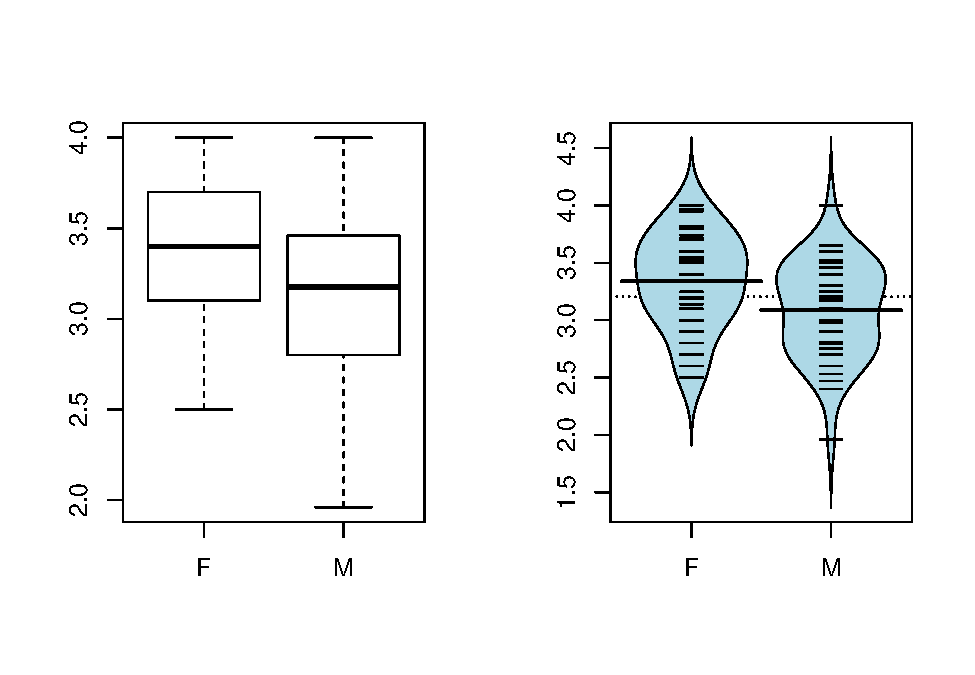
\includegraphics{GreenwoodBanner_files/figure-latex/Figure2-15-1.pdf}
\caption{\label{fig:Figure2-15}Side-by-side boxplot and beanplot of GPAs of STAT 217
students by sex.}
\end{figure}

\begin{Shaded}
\begin{Highlighting}[]
\KeywordTok{mean}\NormalTok{(GPA~Sex, }\DataTypeTok{data=}\NormalTok{s217)}
\end{Highlighting}
\end{Shaded}

\begin{verbatim}
##        F        M 
## 3.338378 3.088571
\end{verbatim}

\begin{Shaded}
\begin{Highlighting}[]
\KeywordTok{favstats}\NormalTok{(GPA~Sex, }\DataTypeTok{data=}\NormalTok{s217)}
\end{Highlighting}
\end{Shaded}

\begin{verbatim}
##   Sex  min  Q1 median   Q3 max     mean        sd  n missing
## 1   F 2.50 3.1  3.400 3.70   4 3.338378 0.4074549 37       0
## 2   M 1.96 2.8  3.175 3.46   4 3.088571 0.4151789 42       0
\end{verbatim}

In these data, the distributions of the GPAs look to be left skewed but
maybe not as dramatically as the responses were right-skewed in the
previous example. The Female GPAs look to be slightly higher than for
Males (0.25 GPA difference in the means) but is that a ``real''
difference? We need our inference tools to more fully assess these
differences.

\begin{Shaded}
\begin{Highlighting}[]
\KeywordTok{diffmean}\NormalTok{(GPA~Sex, }\DataTypeTok{data=}\NormalTok{s217)}
\end{Highlighting}
\end{Shaded}

\begin{verbatim}
##   diffmean 
## -0.2498069
\end{verbatim}

First, we can try the parametric approach:

\begin{Shaded}
\begin{Highlighting}[]
\KeywordTok{t.test}\NormalTok{(GPA~Sex, }\DataTypeTok{data=}\NormalTok{s217, }\DataTypeTok{var.equal=}\NormalTok{T)}
\end{Highlighting}
\end{Shaded}

\begin{verbatim}
## 
##  Two Sample t-test
## 
## data:  GPA by Sex
## t = 2.6919, df = 77, p-value = 0.008713
## alternative hypothesis: true difference in means is not equal to 0
## 95 percent confidence interval:
##  0.06501838 0.43459552
## sample estimates:
## mean in group F mean in group M 
##        3.338378        3.088571
\end{verbatim}

So the test statistic was observed to be \(t=2.69\) and it hopefully
follows a \(t(77)\) distribution under the null hypothesis. This
provides a p-value of 0.008713 that we can trust if all the conditions
to use this procedure are met. Compare these results to the permutation
approach, which relaxes that normality assumption, with the results that
follow. In the permutation test, \(T=2.692\) and the p-value is 0.005
which is a little smaller than the result provided by the parametric
approach. The agreement of the two approaches, again, provides some
re-assurance about the use of either approach.

\begin{Shaded}
\begin{Highlighting}[]
\NormalTok{Tobs <-}\StringTok{ }\KeywordTok{t.test}\NormalTok{(GPA~Sex, }\DataTypeTok{data=}\NormalTok{s217, }\DataTypeTok{var.equal=}\NormalTok{T)$statistic}
\NormalTok{Tstar <-}\StringTok{ }\KeywordTok{matrix}\NormalTok{(}\OtherTok{NA}\NormalTok{, }\DataTypeTok{nrow=}\NormalTok{B)}
\NormalTok{for (b in (}\DecValTok{1}\NormalTok{:B))\{}
  \NormalTok{Tstar[b] <-}\StringTok{ }\KeywordTok{t.test}\NormalTok{(GPA~}\KeywordTok{shuffle}\NormalTok{(Sex), }\DataTypeTok{data=}\NormalTok{s217, }\DataTypeTok{var.equal=}\NormalTok{T)$statistic}
\NormalTok{\}}
\end{Highlighting}
\end{Shaded}




\begin{Shaded}
\begin{Highlighting}[]
\KeywordTok{par}\NormalTok{(}\DataTypeTok{mfrow=}\KeywordTok{c}\NormalTok{(}\DecValTok{1}\NormalTok{,}\DecValTok{2}\NormalTok{))}
\KeywordTok{hist}\NormalTok{(Tstar,}\DataTypeTok{labels=}\NormalTok{T)}
\KeywordTok{abline}\NormalTok{(}\DataTypeTok{v=}\KeywordTok{c}\NormalTok{(-}\DecValTok{1}\NormalTok{,}\DecValTok{1}\NormalTok{)*Tobs, }\DataTypeTok{lwd=}\DecValTok{2}\NormalTok{, }\DataTypeTok{col=}\StringTok{"red"}\NormalTok{)}
\KeywordTok{plot}\NormalTok{(}\KeywordTok{density}\NormalTok{(Tstar), }\DataTypeTok{main=}\StringTok{"Density curve of Tstar"}\NormalTok{)}
\KeywordTok{abline}\NormalTok{(}\DataTypeTok{v=}\KeywordTok{c}\NormalTok{(-}\DecValTok{1}\NormalTok{,}\DecValTok{1}\NormalTok{)*Tobs, }\DataTypeTok{lwd=}\DecValTok{2}\NormalTok{, }\DataTypeTok{col=}\StringTok{"red"}\NormalTok{)}
\end{Highlighting}
\end{Shaded}

\begin{figure}[htbp]
\centering
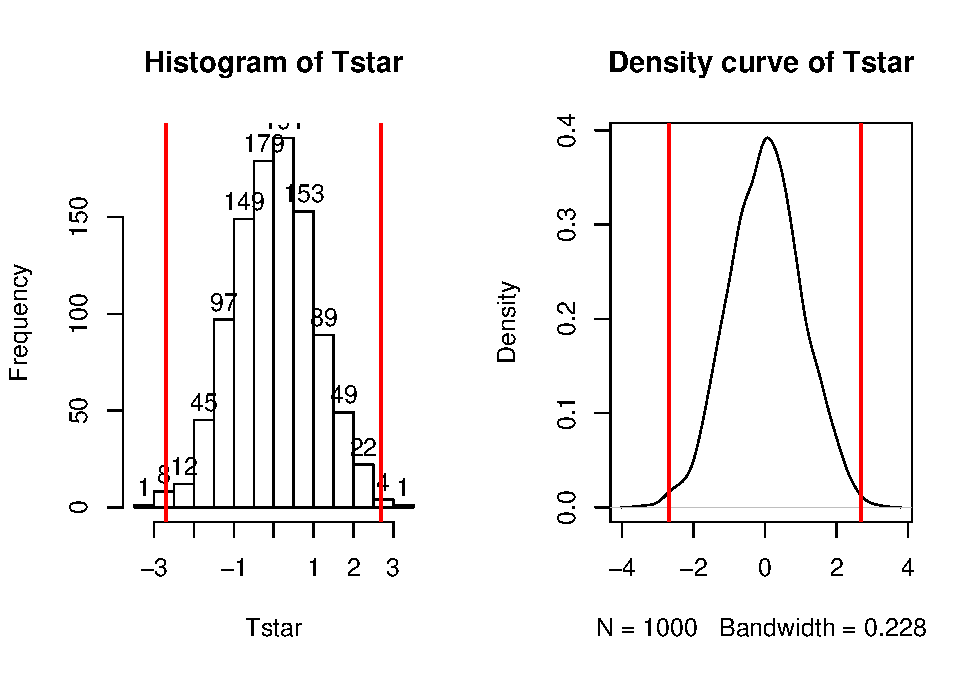
\includegraphics{GreenwoodBanner_files/figure-latex/Figure2-16-1.pdf}
\caption{\label{fig:Figure2-16}Histogram and density curve of permutation distribution of
test statistic for STAT 217 GPAs.}
\end{figure}

\begin{Shaded}
\begin{Highlighting}[]
\KeywordTok{pdata}\NormalTok{(}\KeywordTok{abs}\NormalTok{(Tstar),}\KeywordTok{abs}\NormalTok{(Tobs),}\DataTypeTok{lower.tail=}\NormalTok{F)}
\end{Highlighting}
\end{Shaded}

\begin{verbatim}
##     t 
## 0.005
\end{verbatim}

Here is a full write-up of the results using all 6+ hypothesis testing
steps, using the permutation results:

\begin{enumerate}
\def\labelenumi{\arabic{enumi}.}
\setcounter{enumi}{-1}
\item
  \emph{Isolate the claim to be proved and method to use (define a test
  statistic T)} We want to test for a difference in the means between
  males and females and will use the equal-variance two-sample t-test
  statistic to compare them, making a decision at the 5\% significance
  level.
\item
  Write the null and alternative hypotheses

  \begin{itemize}
  \item
    \(H_0: \mu_{male} = \mu_{female}\)

    \begin{itemize}
    \tightlist
    \item
      where \(\mu_{male}\) is the true mean GPA for males and
      \(\mu_{female}\) is true mean GPA for females.
    \end{itemize}
  \item
    \(H_A: \mu_{male} \ne \mu_{female}\)
  \end{itemize}
\item
  Check conditions for the procedure being used

  \begin{itemize}
  \item
    \textbf{Independent observations condition}: It appears that this
    assumption is met because there is no reason to assume any
    clustering or grouping of responses that might create dependence in
    the observations. The only possible consideration is that the
    observations were taken from different sections and there could be
    some differences between the sections. However, for overall GPA this
    not likely to be a big issue. The only way this could create a
    violation here is if certain sections tended to attract students
    with different GPA levels (such as the 9 am section had the
    best/worst GPA students\ldots{}).
  \item
    \textbf{Equal variance condition} : There is a small difference in
    the range of the observations in the two groups but the standard
    deviations are very similar so there is no evidence that this
    condition is violated.
  \item
    \textbf{Similar distribution condition}: Based on the side-by-side
    boxplots and beanplots, it appears that both groups have slightly
    left-skewed distributions, which could be problematic for the
    parametric approach, but the permutation approach condition is not
    violated since the distributions look to have fairly similar shapes.
  \end{itemize}
\item
  Find the value of the appropriate test statistic

  \begin{itemize}
  \tightlist
  \item
    \(T=2.69\) from the previous R output.
  \end{itemize}
\item
  Find the p-value

  \begin{itemize}
  \item
    p-value=0.005 from the permutation distribution results.
  \item
    This means that there is about a 0.5\% chance we would observe a
    difference in mean GPA (female-male or male-female) of 0.25 points
    or more if there in fact no difference in true mean GPA between
    females and males in STAT 217 in a particular semester.
  \end{itemize}
\item
  Decision

  \begin{itemize}
  \tightlist
  \item
    Since the p-value is ``small'' (\emph{a priori} 5\% significance
    level selected), we can reject the null hypothesis.
  \end{itemize}
\item
  Conclusion and scope of inference, specific to the problem

  \begin{itemize}
  \item
    There is strong evidence against the null hypothesis of no
    difference in the true mean GPA between males and females for the
    STAT 217 students in this semester and so we conclude that there is
    evidence of a difference in the mean GPAs between males and females
    in STAT 217 students.
  \item
    Because this was not a randomized experiment, we can't say that the
    difference in sex causes the difference in mean GPA and because it
    was not a random sample from a larger population, our inferences
    only pertain the STAT 217 students that responded to the survey in
    that semester.
  \end{itemize}
\end{enumerate}

\section{Confidence intervals and bootstrapping}\label{section2-8}

Randomly shuffling the treatments between the observations is like
randomly sampling the treatments without replacement. In other words, we
randomly sample one observation at a observations. This provides us with
a technique for testing hypotheses because it provides new splits of the
observations into groups that are as interesting as what we observed if
the null hypothesis is assumed true. In most situations, we also want to
estimate parameters of interest and provide \textbf{\emph{confidence
intervals}} for those parameters (an interval where we are \_\_\%
\textbf{\emph{confident}} that the true parameter lies). As before,
there are two options we will consider -- a parametric and a
nonparametric approach. The nonparametric approach will be using what is
called \textbf{\emph{bootstrapping}} and draws its name from ``pull
yourself up by your bootstraps'' where you improve your situation based
on your own efforts. In statistics, we make our situation or inferences
better by re-using the observations we have by assuming that the sample
represents the population. Since each observation represents other
similar observations in the population that we didn't get to measure, if
we \textbf{\emph{sample with replacement}} to generate a new data set of
size \emph{n} from our data set (also of size \emph{n}) it mimics the
process of taking our population of interest. This process also ends up
giving us useful sampling distributions of statistics even when our
standard normality assumption is violated, similar to what we
encountered in the permutation tests. Bootstrapping is especially useful
in situations where we are interested in statistics other than the mean
(say we want a confidence interval for a median or a standard deviation)
or when we consider functions of more than one parameter and don't want
to derive the distribution of the statistic (say the difference in two
medians). In this text, bootstrapping is used to provide more
trustworthy inferences when some of our assumptions (especially
normality) might be violated for our parametric procedure.

To perform bootstrapping, we will use the \texttt{resample} function
from the \texttt{mosaic} package. We can apply this function to a data
set and get a new version of the data set by sampling new observations
\emph{with replacement} from the original one. The new, bootstrapped
version of the data set (called \texttt{MockJury\_BTS} below) contains a
new variable called \texttt{orig.\ id} which is the number of the
subject from the original data set. By summarizing how often each of
these id's occurred in a bootstrapped data set, we can see how the
re-sampling works. The \texttt{table} function will count up how many
times each observation was used in the bootstrap sample, providing a row
with the id followed by a row with the count\footnote{The
  \texttt{as.numeric} function is also used here. It really isn't
  important but makes sure the output of \texttt{table} is sorted by
  observation number by first converting the \emph{orig.id} variable
  into a numeric vector.}. In the first bootstrap sample shown, the 2nd,
7th, and 9th observations were sampled one time each, the 4th
observation was sampled three times, and the 1st, 3rd, 5th, and many
others were not sampled at all. Bootstrap sampling thus picks some
observations multiple times and to do that it has to ignore some
observations.

\begin{Shaded}
\begin{Highlighting}[]
\NormalTok{MockJury_BTS <-}\StringTok{ }\KeywordTok{resample}\NormalTok{(MockJury2)}
\KeywordTok{table}\NormalTok{(}\KeywordTok{as.numeric}\NormalTok{(MockJury_BTS$orig.id))}
\end{Highlighting}
\end{Shaded}

\begin{verbatim}
## 
##  1  2  3  4  5  6 10 11 12 14 15 17 18 19 20 22 24 26 29 30 32 35 36 37 39 
##  1  2  2  1  3  2  1  2  1  1  3  1  2  1  2  1  2  1  2  2  2  2  1  2  2 
## 40 42 43 44 45 46 47 48 49 55 58 59 60 61 69 70 71 72 74 75 
##  2  1  1  4  2  2  1  2  1  2  1  1  2  2  2  2  2  1  1  1
\end{verbatim}

Like in permutations, one randomization isn't enough. A second bootstrap
sample is also provided to help you get a sense of what it is doing to
generate a data set. It did not select subject 7 but did select 2, 4, 6,
and 8 two times. You can see other variations in the resulting
re-sampling of subjects with the most sampled subject being the chance
of selecting any observation for any slot in the new data set is
\(1/75\) and the expected or mean number of appearances we expect to see
for an observation is the number of tries times the probably of
selection on each so \(75*1/75=1\).

\begin{Shaded}
\begin{Highlighting}[]
\NormalTok{MockJury_BTS2 <-}\StringTok{ }\KeywordTok{resample}\NormalTok{(MockJury2)}
\KeywordTok{table}\NormalTok{(}\KeywordTok{as.numeric}\NormalTok{(MockJury_BTS2$orig.id))}
\end{Highlighting}
\end{Shaded}

\begin{verbatim}
## 
##  1  2  3  5  6  8 11 12 13 14 15 18 19 20 21 23 24 26 27 28 29 31 32 34 36 
##  1  1  1  1  4  1  1  1  1  3  1  1  1  1  3  2  2  1  1  1  2  1  2  1  2 
## 37 38 40 42 46 48 50 51 52 56 58 59 61 62 63 66 67 68 69 72 73 74 75 
##  1  2  1  1  1  2  4  1  1  1  3  2  1  1  1  1  1  1  2  3  1  4  2
\end{verbatim}

We can use the two results to get an idea of distribution of results in
terms of number of times observations might be re-sampled when sampling
with replacement and the variation in those results, as shown in Figure
\ref{fig:Figure2-17}. We could also derive the expected counts for each
number of times of re-sampling when we start with all observations
having an equal chance and sampling with replacement but this isn't
important for using bootstrapping methods.




\begin{figure}[htbp]
\centering
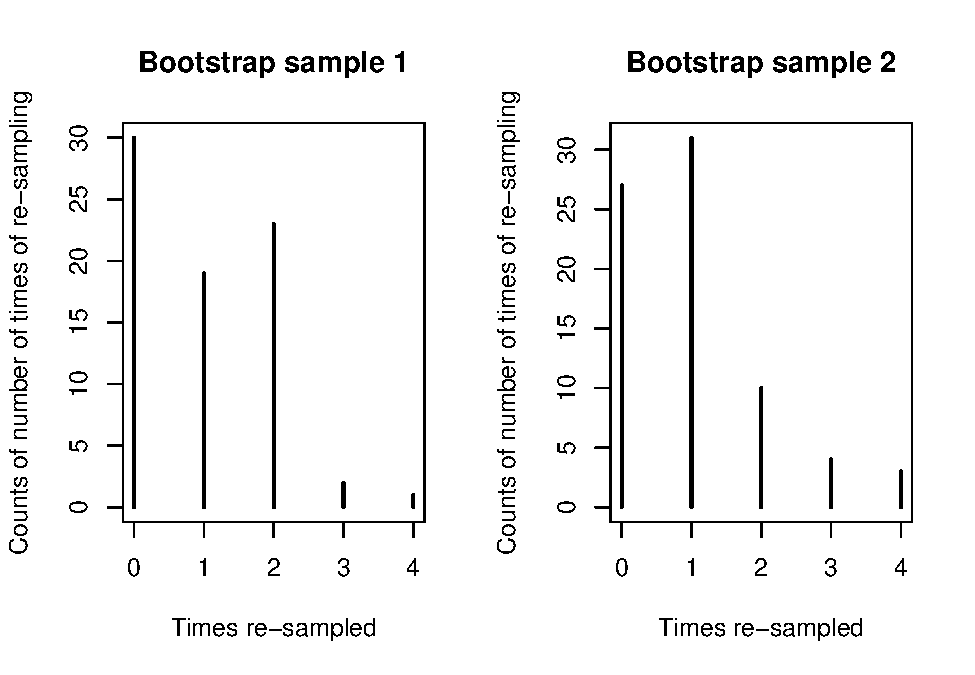
\includegraphics{GreenwoodBanner_files/figure-latex/Figure2-17-1.pdf}
\caption{\label{fig:Figure2-17}Counts of number of times of observation (or not observed
for times re-sampled of 0) for two bootstrap samples.}
\end{figure}

The main point of this exploration was to see that each run of the
\texttt{resample} function provides a new version of the data set.
Repeating this \(B\) times using another \texttt{for} loop, we will
track our quantity of interest, say \(T\), in all these new ``data
sets'' and call those results \(T^*\). The distribution of the
bootstrapped \(T^*\) statistics will tell us about the range of results
to expect for the statistic and the middle \_\_\% of the \(T^*\)'s
provides a\\
\textbf{\emph{bootstrap confidence interval}}\footnote{There are
  actually many ways to use this information to make a confidence
  interval. We are using the simplest method that is called the
  ``percentile'' method.} for the true parameter -- here the
\emph{difference in the two population means}.

To make this concrete, we can revisit our previous examples, starting
with the \texttt{MockJury2} data created before and our interest in
comparing the mean sentences for the \emph{Average}and
\emph{Unattractive} picture groups. The bootstrapping code is very
similar to the permutation code except that we apply the
\texttt{resample} function to the entire data set as opposed to the
\texttt{shuffle} function being applied to the explanatory variable.





\begin{Shaded}
\begin{Highlighting}[]
\KeywordTok{par}\NormalTok{(}\DataTypeTok{mfrow=}\KeywordTok{c}\NormalTok{(}\DecValTok{1}\NormalTok{,}\DecValTok{2}\NormalTok{))}
\NormalTok{Tobs <-}\StringTok{ }\KeywordTok{diffmean}\NormalTok{(Years ~}\StringTok{ }\NormalTok{Attr, }\DataTypeTok{data=}\NormalTok{MockJury2); Tobs}
\NormalTok{B <-}\StringTok{ }\DecValTok{1000}
\NormalTok{Tstar <-}\StringTok{ }\KeywordTok{matrix}\NormalTok{(}\OtherTok{NA}\NormalTok{,}\DataTypeTok{nrow=}\NormalTok{B)}
\NormalTok{for (b in (}\DecValTok{1}\NormalTok{:B))\{}
  \NormalTok{Tstar[b] <-}\StringTok{ }\KeywordTok{diffmean}\NormalTok{(Years ~}\StringTok{ }\NormalTok{Attr, }\DataTypeTok{data=}\KeywordTok{resample}\NormalTok{(MockJury2))}
  \NormalTok{\}}
\KeywordTok{hist}\NormalTok{(Tstar, }\DataTypeTok{labels=}\NormalTok{T)}
\KeywordTok{abline}\NormalTok{(}\DataTypeTok{v=}\NormalTok{Tobs, }\DataTypeTok{col=}\StringTok{"red"}\NormalTok{, }\DataTypeTok{lwd=}\DecValTok{2}\NormalTok{)}
\KeywordTok{plot}\NormalTok{(}\KeywordTok{density}\NormalTok{(Tstar), }\DataTypeTok{main=}\StringTok{"Density curve of Tstar"}\NormalTok{)}
\KeywordTok{abline}\NormalTok{(}\DataTypeTok{v=}\NormalTok{Tobs, }\DataTypeTok{col=}\StringTok{"red"}\NormalTok{, }\DataTypeTok{lwd=}\DecValTok{2}\NormalTok{)}
\end{Highlighting}
\end{Shaded}

\begin{figure}[htbp]
\centering
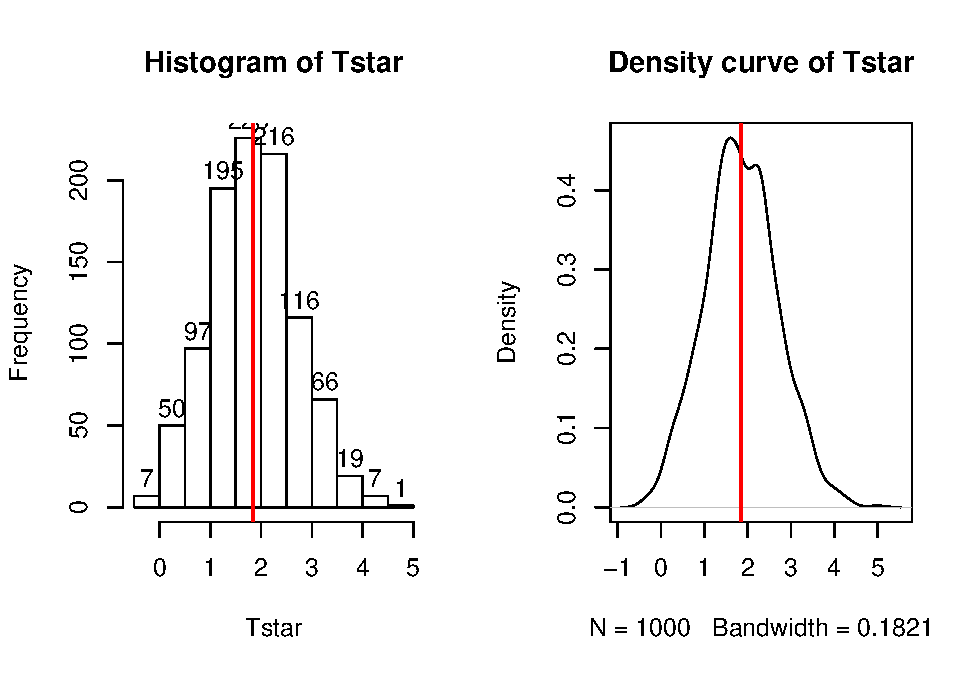
\includegraphics{GreenwoodBanner_files/figure-latex/Figure2-18-1.pdf}
\caption{\label{fig:Figure2-18}Histogram and density curve of bootstrap distributions of
difference in sample mean \texttt{Years} with vertical line for the
observed difference in the means of 1.84 years.}
\end{figure}

\begin{Shaded}
\begin{Highlighting}[]
\KeywordTok{favstats}\NormalTok{(Tstar)}
\end{Highlighting}
\end{Shaded}

\begin{verbatim}
## diffmean 
## 1.837127 
##         min       Q1   median       Q3      max     mean        sd    n
##  -0.3627312 1.305773 1.833091 2.385281 4.988756 1.854428 0.8438987 1000
##  missing
##        0
\end{verbatim}

In this situation, the observed difference in the mean sentences is 1.84
years (Unattractive-Average), which is the vertical line in Figure
\ref{fig:Figure2-18}. The bootstrap distribution shows the results for
the difference in the sample means when fake data sets are
re-constructed by sampling from the data set with replacement. The
bootstrap distribution is approximately centered at the observed value
(difference in the sample means) and is relatively symmetric.

The permutation distribution in the same situation (Figure
\ref{fig:Figure2-12}) had a similar shape but was centered at 0.
Permutations create sampling distributions based on assuming the null
hypothesis is true, which is useful for hypothesis testing.
Bootstrapping creates distributions centered at the observed result,
which is the sampling distribution ``under the alternative'' or when no
null hypothesis is assumed; bootstrap distributions are useful for
generating confidence intervals for the true parameter values.

To create a 95\% bootstrap confidence interval for the difference in the
true mean sentences (\(\mu_{Unattr}-\mu_{Avg}\)), select the middle 95\%
of results from the bootstrap distribution. Specifically, find the 2.5th
percentile and the 97.5th percentile (values that put 2.5 and 97.5\% of
the results to the left) in the bootstrap distribution, which leaves
95\% in the middle for the confidence interval. To find percentiles in a
distribution in R, functions are of the form
\texttt{q{[}Name\ of\ distribution{]}}, with the function \texttt{qt}
extracting percentiles from a \(t\)-distribution (examples below). From
the bootstrap results, use the \texttt{qdata} function on the
\texttt{Tstar} results that contain the bootstrap distribution of the
statistic of interest.

\begin{Shaded}
\begin{Highlighting}[]
\KeywordTok{qdata}\NormalTok{(Tstar, }\FloatTok{0.025}\NormalTok{)}
\end{Highlighting}
\end{Shaded}

\begin{verbatim}
##         p  quantile 
## 0.0250000 0.2414232
\end{verbatim}

\begin{Shaded}
\begin{Highlighting}[]
\KeywordTok{qdata}\NormalTok{(Tstar, }\FloatTok{0.975}\NormalTok{)}
\end{Highlighting}
\end{Shaded}

\begin{verbatim}
##        p quantile 
## 0.975000 3.521528
\end{verbatim}

These results tell us that the 2.5th percentile of the bootstrap
distribution is at 0.26 years and the 97.5th percentile is at 3.50
years. We can combine these results to provide a 95\% confidence for
\(\mu_{Unattr}-\mu_{Avg}\) that is between 0.26 and 3.50. We can
interpret this as with any confidence interval, that we are 95\%
confident that the difference in the true mean suggested sentences
(Unattractive minus Average group) is between 0.26 and 3.50 years. We
can also obtain both percentiles in one line of code using:

\begin{Shaded}
\begin{Highlighting}[]
\NormalTok{quantiles <-}\StringTok{ }\KeywordTok{qdata}\NormalTok{(Tstar, }\KeywordTok{c}\NormalTok{(}\FloatTok{0.025}\NormalTok{,}\FloatTok{0.975}\NormalTok{))}
\NormalTok{quantiles}
\end{Highlighting}
\end{Shaded}

\begin{verbatim}
##        quantile     p
## 2.5%  0.2414232 0.025
## 97.5% 3.5215278 0.975
\end{verbatim}

Figure \ref{fig:Figure2-19} displays those same percentiles on the
bootstrap distribution residing in \texttt{Tstar}.




\begin{Shaded}
\begin{Highlighting}[]
\KeywordTok{par}\NormalTok{(}\DataTypeTok{mfrow=}\KeywordTok{c}\NormalTok{(}\DecValTok{1}\NormalTok{,}\DecValTok{2}\NormalTok{))}
\KeywordTok{hist}\NormalTok{(Tstar, }\DataTypeTok{labels=}\NormalTok{T)}
\KeywordTok{abline}\NormalTok{(}\DataTypeTok{v=}\NormalTok{quantiles$quantile, }\DataTypeTok{col=}\StringTok{"blue"}\NormalTok{, }\DataTypeTok{lwd=}\DecValTok{3}\NormalTok{)}
\KeywordTok{plot}\NormalTok{(}\KeywordTok{density}\NormalTok{(Tstar), }\DataTypeTok{main=}\StringTok{"Density curve of Tstar"}\NormalTok{)}
\KeywordTok{abline}\NormalTok{(}\DataTypeTok{v=}\NormalTok{quantiles$quantile, }\DataTypeTok{col=}\StringTok{"blue"}\NormalTok{, }\DataTypeTok{lwd=}\DecValTok{3}\NormalTok{)}
\end{Highlighting}
\end{Shaded}

\begin{figure}[htbp]
\centering
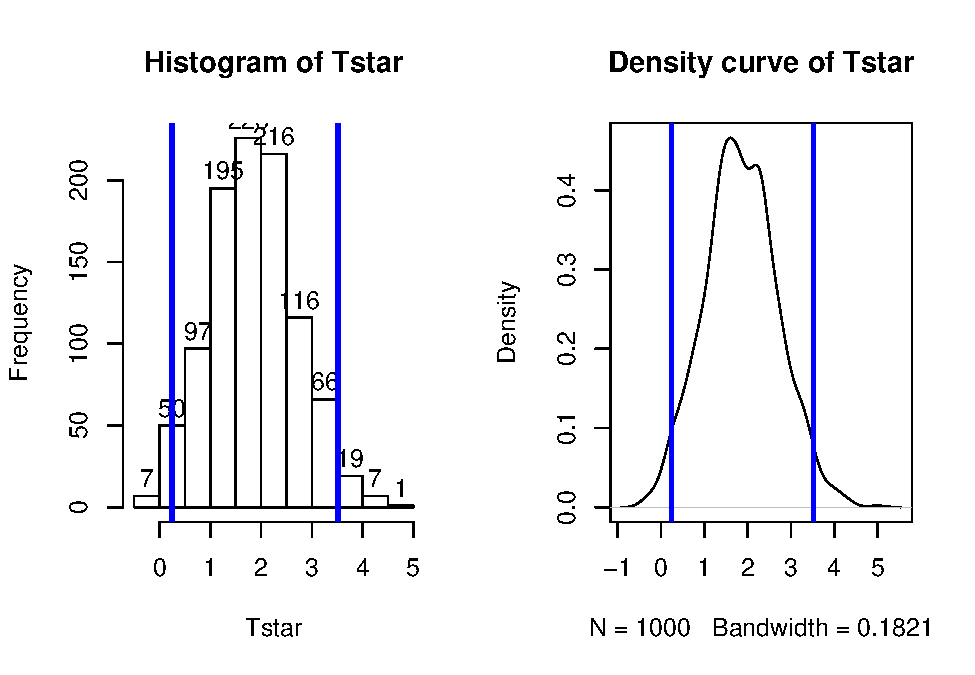
\includegraphics{GreenwoodBanner_files/figure-latex/Figure2-19-1.pdf}
\caption{\label{fig:Figure2-19}Histogram and density curve of bootstrap distribution with
95\% bootstrap confidence intervals displayed (vertical lines).}
\end{figure}

Although confidence intervals can exist without referencing hypotheses,
we can revisit our previous \(H_0: \mu_{Unattr} = \mu_{Avg}\). This null
hypothesis is equivalent to testing
\(H_0: \mu_{Unattr} - \mu_{Avg} = 0\), that the difference in the true
means is equal to 0 years. And the difference in the means was the scale
for our confidence interval, which did not contain 0 years. We will call
0 an interesting \textbf{\emph{reference value}} for the confidence
interval, because here it is the value where the true means are equal to
each other (have a difference of 0 years). In general, if our confidence
interval does not contain 0, then it is saying that 0 is not one of our
likely values for the difference in the true means. This implies that we
should reject a claim that they are equal. This provides the same
inferences for the hypotheses that we considered previously using both a
parametric and permutation approach. The general summary is that we can
use confidence intervals to test hypotheses by assessing whether the
reference value under the null hypothesis is in the confidence interval
(FTR \(H_0\)) or outside the confidence interval (Reject \(H_0\)).
P-values are more informative about hypotheses but confidence intervals
are more information about the size of differences, so both offer useful
information and, as shown here, can provide consistent conclusions about
hypotheses.

As in the previous situation, we also want to consider the parametric
approach for comparison purposes and to have that method available,
especially to help us understand some methods where we will only
consider parametric inferences in later chapters. The parametric
confidence interval is called the \textbf{\emph{equal variance,
two-sample t confidence interval}} and assumes that the populations
being sampled from are normally distributed and leads to using a
\(t\)-distribution to form the interval. The output from the
\texttt{t.test} function provides the parametric 95\% confidence
interval calculated for you:

\begin{Shaded}
\begin{Highlighting}[]
\KeywordTok{t.test}\NormalTok{(Years ~}\StringTok{ }\NormalTok{Attr, }\DataTypeTok{data=}\NormalTok{MockJury2, }\DataTypeTok{var.equal=}\NormalTok{T)}
\end{Highlighting}
\end{Shaded}

\begin{verbatim}
## 
##  Two Sample t-test
## 
## data:  Years by Attr
## t = -2.1702, df = 73, p-value = 0.03324
## alternative hypothesis: true difference in means is not equal to 0
## 95 percent confidence interval:
##  -3.5242237 -0.1500295
## sample estimates:
##      mean in group Average mean in group Unattractive 
##                   3.973684                   5.810811
\end{verbatim}

The \texttt{t.test} function again switched the order of the groups and
provides slightly different end-points than our bootstrap confidence
interval (both are made at the 95\% confidence level though), which was
slightly narrower. Both intervals have the same interpretation, only the
methods for calculating the intervals and the assumptions differ.
Specifically, the bootstrap interval can tolerate different distribution
shapes other than normal and still provide intervals that work
well\footnote{When hypothesis tests ``work well'' they have high power
  to detect differences while having Type I error rates that are close
  to what we choose a priori. When confidence intervals ``work well'',
  they contain the true parameter value in repeated random samples at
  around the selected confidence level}. The other assumptions are all
the same as for the hypothesis test, where we continue to assume that we
have independent observations with equal variances for the two groups.

The formula that \texttt{t.test} is using to calculate the parametric
\textbf{\emph{equal-variance two-sample t confidence interval}} is:

\[\bar{x}_1 - \bar{x}_2 \mp t^*_{df}s_p\sqrt{\frac{1}{n_1}+\frac{1}{n_2}}\]

In this situation, the \emph{df} is again \(n_1+n_2-2\) and
\(s_p = \sqrt{\frac{(n_1-1)s_1^2 + (n_2-1)s_2^2}{n_1+n_2-2}}\). The
\(t^*_{df}\) is a multiplier that comes from finding the percentile from
the \(t\)-distribution that puts \(C\)\% in the middle of the
distribution with \(C\) being the confidence level. It is important to
note that this \(t^*\) has nothing to do with the previous test
statistic \(t\). It is confusing and many of you will, at some point,
happily take the result from a test statistic calculation and use it for
a multiplier in a \(t\)-based confidence interval. Figure
\ref{fig:Figure2-20} shows the \(t\)-distribution with 73 degrees of
freedom and the cut-offs that put 95\% of the area in the middle.




\begin{Shaded}
\begin{Highlighting}[]
\KeywordTok{par}\NormalTok{(}\DataTypeTok{mfrow=}\KeywordTok{c}\NormalTok{(}\DecValTok{1}\NormalTok{,}\DecValTok{1}\NormalTok{))}
\NormalTok{x<-}\KeywordTok{seq}\NormalTok{(}\DataTypeTok{from=}\NormalTok{-}\DecValTok{4}\NormalTok{,}\DataTypeTok{to=}\DecValTok{4}\NormalTok{,}\DataTypeTok{length.out=}\DecValTok{200}\NormalTok{)}
\KeywordTok{plot}\NormalTok{(x,}\KeywordTok{dt}\NormalTok{(x,}\DataTypeTok{df=}\DecValTok{73}\NormalTok{),}\DataTypeTok{col=}\StringTok{"red"}\NormalTok{,}\DataTypeTok{lty=}\DecValTok{2}\NormalTok{,}\DataTypeTok{lwd=}\DecValTok{3}\NormalTok{,}\DataTypeTok{type=}\StringTok{"l"}\NormalTok{,}\DataTypeTok{xlab=}\StringTok{"t-values"}\NormalTok{,}\DataTypeTok{ylab=}\StringTok{"Density"}\NormalTok{,}
     \DataTypeTok{main=}\StringTok{"Plot of t(73) distribution"} \NormalTok{)}
\KeywordTok{abline}\NormalTok{(}\DataTypeTok{v=}\NormalTok{-}\FloatTok{2.1702}\NormalTok{,}\DataTypeTok{lwd=}\DecValTok{3}\NormalTok{)}
\KeywordTok{abline}\NormalTok{(}\DataTypeTok{v=}\FloatTok{2.1702}\NormalTok{,}\DataTypeTok{lwd=}\DecValTok{3}\NormalTok{)}
\end{Highlighting}
\end{Shaded}

\begin{figure}[htbp]
\centering
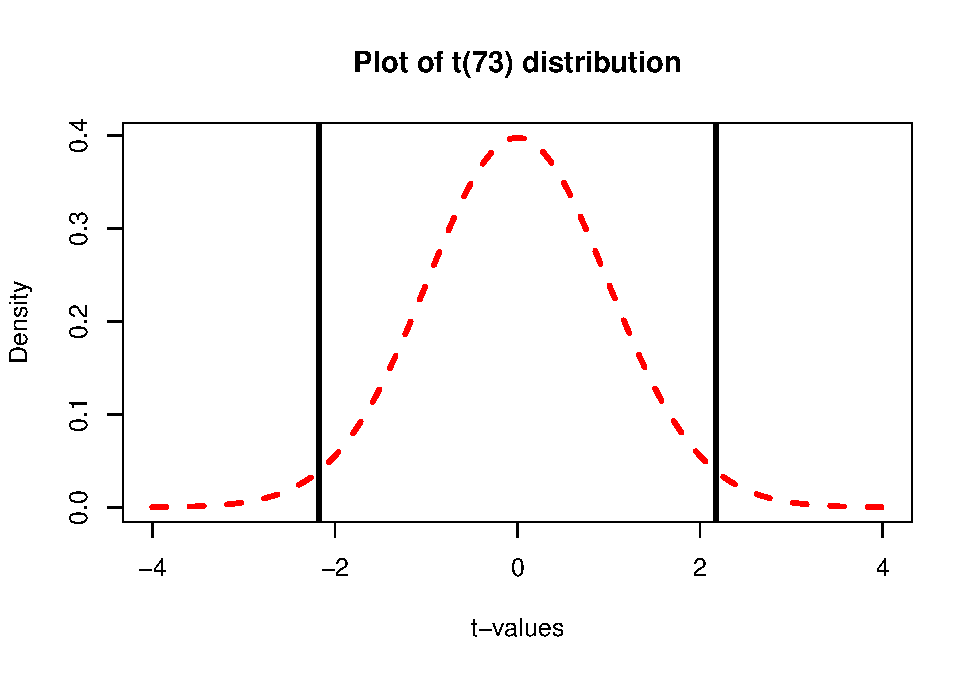
\includegraphics{GreenwoodBanner_files/figure-latex/Figure2-20-1.pdf}
\caption{\label{fig:Figure2-20}Plot of \(t(73)\) with cut-offs for putting 95\% of
distributions in the middle.}
\end{figure}

For 95\% confidence intervals, the multiplier is going to be close to 2
and anything else is a sign of a mistake. We can use R to get the
multipliers for confidence intervals using the \texttt{qt} function in a
similar fashion to how \texttt{qdata} was used in the bootstrap results,
except that this new value must be used in the previous confidence
interval formula. This function produces values for requested
percentiles, so if we want to put 95\% in the middle, we place 2.5\% in
each tail of the distribution and need to request the 97.5th percentile.
Because the \(t\)-distribution is always symmetric around 0, we merely
need to look up the value for the 97.5th percentile and know that the
multiplier for the 2.5th percentile is just \(-t^*\). The \(t^*\)
multiplier to form the confidence interval is 1.993 for a 95\%
confidence interval when the \(df=73\) based on the results from
\texttt{qt}:

\begin{Shaded}
\begin{Highlighting}[]
\KeywordTok{qt}\NormalTok{(}\FloatTok{0.975}\NormalTok{, }\DataTypeTok{df=}\DecValTok{73}\NormalTok{)}
\end{Highlighting}
\end{Shaded}

\begin{verbatim}
## [1] 1.992997
\end{verbatim}

Note that the 2.5th percentile is just the negative of this value due to
symmetry and the real source of the minus in the minus/plus in the
formula for the confidence interval.

\begin{Shaded}
\begin{Highlighting}[]
\KeywordTok{qt}\NormalTok{(}\FloatTok{0.025}\NormalTok{, }\DataTypeTok{df=}\DecValTok{73}\NormalTok{)}
\end{Highlighting}
\end{Shaded}

\begin{verbatim}
## [1] -1.992997
\end{verbatim}

We can also re-write the confidence interval formula into a slightly
more general form as

\[\bar{x}_1 - \bar{x}_2 \mp t^*_{df}SE_{\bar{x}_1 - \bar{x}_2}\ \text{ OR }\ 
\bar{x}_1 - \bar{x}_2 \mp ME\]

where
\(SE_{\bar{x}_1 - \bar{x}_2} = s_p\sqrt{\frac{1}{n_1}+\frac{1}{n_2}}\)
and \(ME = t^*_{df}SE_{\bar{x}_1 - \bar{x}_2}\). In some situations,
researchers will report the \textbf{\emph{standard error}} (SE) or
\textbf{\emph{margin of error}} (ME) as a method of quantifying the
uncertainty in a statistic. The SE is an estimate of the standard
deviation of the statistic (here \(\bar{x}_1 - \bar{x}_2\)) and the ME
is an estimate of the precision of a statistic that can be used to
directly form a confidence interval. The ME depends on the choice of
confidence level although 95\% is almost always selected.

To finish this example, R can be used to help you do calculations much
like a calculator except with much more power ``under the hood''. You
have to make sure you are careful with using \texttt{(\ )} to group
items and remember that the asterisk (*) is used for multiplication in
R. We need the pertinent information which is available from the
\texttt{favstats} output. Two versions of this output are provided
below, the first is how the output appears directly from R, the second
is a formatted table has the relevant information bolded which is needed
to calculate the confidence interval ``by hand'' using R.

\begin{Shaded}
\begin{Highlighting}[]
\KeywordTok{favstats}\NormalTok{(Years~Attr, }\DataTypeTok{data=}\NormalTok{MockJury2)}
\end{Highlighting}
\end{Shaded}

\begin{verbatim}
##           Attr min Q1 median Q3 max     mean       sd  n missing
## 1      Average   1  2      3  5  12 3.973684 2.823519 38       0
## 2 Unattractive   1  2      5 10  15 5.810811 4.364235 37       0
\end{verbatim}

\begin{longtable}[]{@{}cccccccccc@{}}
\toprule
\begin{minipage}[b]{0.15\columnwidth}\centering\strut
Attr\strut
\end{minipage} & \begin{minipage}[b]{0.05\columnwidth}\centering\strut
min\strut
\end{minipage} & \begin{minipage}[b]{0.04\columnwidth}\centering\strut
Q1\strut
\end{minipage} & \begin{minipage}[b]{0.08\columnwidth}\centering\strut
median\strut
\end{minipage} & \begin{minipage}[b]{0.04\columnwidth}\centering\strut
Q3\strut
\end{minipage} & \begin{minipage}[b]{0.05\columnwidth}\centering\strut
max\strut
\end{minipage} & \begin{minipage}[b]{0.08\columnwidth}\centering\strut
mean\strut
\end{minipage} & \begin{minipage}[b]{0.08\columnwidth}\centering\strut
sd\strut
\end{minipage} & \begin{minipage}[b]{0.06\columnwidth}\centering\strut
n\strut
\end{minipage} & \begin{minipage}[b]{0.08\columnwidth}\centering\strut
missing\strut
\end{minipage}\tabularnewline
\midrule
\endhead
\begin{minipage}[t]{0.15\columnwidth}\centering\strut
\textbf{Average}\strut
\end{minipage} & \begin{minipage}[t]{0.05\columnwidth}\centering\strut
1\strut
\end{minipage} & \begin{minipage}[t]{0.04\columnwidth}\centering\strut
2\strut
\end{minipage} & \begin{minipage}[t]{0.08\columnwidth}\centering\strut
3\strut
\end{minipage} & \begin{minipage}[t]{0.04\columnwidth}\centering\strut
5\strut
\end{minipage} & \begin{minipage}[t]{0.05\columnwidth}\centering\strut
12\strut
\end{minipage} & \begin{minipage}[t]{0.08\columnwidth}\centering\strut
\textbf{3.97}\strut
\end{minipage} & \begin{minipage}[t]{0.08\columnwidth}\centering\strut
\textbf{2.82}\strut
\end{minipage} & \begin{minipage}[t]{0.06\columnwidth}\centering\strut
\textbf{38}\strut
\end{minipage} & \begin{minipage}[t]{0.08\columnwidth}\centering\strut
0\strut
\end{minipage}\tabularnewline
\begin{minipage}[t]{0.15\columnwidth}\centering\strut
\textbf{Unattractive}\strut
\end{minipage} & \begin{minipage}[t]{0.05\columnwidth}\centering\strut
1\strut
\end{minipage} & \begin{minipage}[t]{0.04\columnwidth}\centering\strut
2\strut
\end{minipage} & \begin{minipage}[t]{0.08\columnwidth}\centering\strut
5\strut
\end{minipage} & \begin{minipage}[t]{0.04\columnwidth}\centering\strut
10\strut
\end{minipage} & \begin{minipage}[t]{0.05\columnwidth}\centering\strut
15\strut
\end{minipage} & \begin{minipage}[t]{0.08\columnwidth}\centering\strut
\textbf{5.81}\strut
\end{minipage} & \begin{minipage}[t]{0.08\columnwidth}\centering\strut
\textbf{4.36}\strut
\end{minipage} & \begin{minipage}[t]{0.06\columnwidth}\centering\strut
\textbf{37}\strut
\end{minipage} & \begin{minipage}[t]{0.08\columnwidth}\centering\strut
0\strut
\end{minipage}\tabularnewline
\bottomrule
\end{longtable}

Start with typing the following command to calculate \(s_p\) and store
it in a variable named \texttt{sp}:

\begin{Shaded}
\begin{Highlighting}[]
\NormalTok{sp <-}\StringTok{ }\KeywordTok{sqrt}\NormalTok{(((}\DecValTok{38-1}\NormalTok{)*(}\FloatTok{2.8235}\NormalTok{^}\DecValTok{2}\NormalTok{)+(}\DecValTok{37-1}\NormalTok{)*(}\FloatTok{4.364}\NormalTok{^}\DecValTok{2}\NormalTok{))/(}\DecValTok{38+37-2}\NormalTok{))}
\NormalTok{sp}
\end{Highlighting}
\end{Shaded}

\begin{verbatim}
## [1] 3.665036
\end{verbatim}

Then calculate the confidence interval that \texttt{t.test} provided
using:

\begin{Shaded}
\begin{Highlighting}[]
\FloatTok{3.974-5.811}\NormalTok{+}\KeywordTok{c}\NormalTok{(-}\DecValTok{1}\NormalTok{,}\DecValTok{1}\NormalTok{)*}\KeywordTok{qt}\NormalTok{(.}\DecValTok{975}\NormalTok{,}\DataTypeTok{df=}\DecValTok{73}\NormalTok{)*sp*}\KeywordTok{sqrt}\NormalTok{(}\DecValTok{1}\NormalTok{/}\DecValTok{38+1}\NormalTok{/}\DecValTok{37}\NormalTok{)}
\end{Highlighting}
\end{Shaded}

\begin{verbatim}
## [1] -3.5240302 -0.1499698
\end{verbatim}

The previous code uses \texttt{c(-1,\ 1)} times the margin of error to
subtract and add the ME to the difference in the sample means
(\(3.974-5.811\)), which generates the lower and then upper bounds of
the confidence interval. If desired, we can also use just the last
portion of the previous calculation to find the margin of error, which
is 1.69 here.

\begin{Shaded}
\begin{Highlighting}[]
\KeywordTok{qt}\NormalTok{(.}\DecValTok{975}\NormalTok{,}\DataTypeTok{df=}\DecValTok{73}\NormalTok{)*sp*}\KeywordTok{sqrt}\NormalTok{(}\DecValTok{1}\NormalTok{/}\DecValTok{38+1}\NormalTok{/}\DecValTok{37}\NormalTok{)}
\end{Highlighting}
\end{Shaded}

\begin{verbatim}
## [1] 1.68703
\end{verbatim}

\section{Bootstrap confidence intervals for difference in
GPAs}\label{section2-9}

We can now apply the new confidence interval methods on the STAT 217
grade data. This time we start with the parametric 95\% confidence
interval ``by hand'' in R and then use \texttt{t.\ test} to verify our
result. The \texttt{favstats} output provides us with the required
information to calculate the confidence interval:

\begin{Shaded}
\begin{Highlighting}[]
\KeywordTok{favstats}\NormalTok{(GPA~Sex,}\DataTypeTok{data=}\NormalTok{s217)}
\end{Highlighting}
\end{Shaded}

\begin{verbatim}
##   Sex  min  Q1 median   Q3 max     mean        sd  n missing
## 1   F 2.50 3.1  3.400 3.70   4 3.338378 0.4074549 37       0
## 2   M 1.96 2.8  3.175 3.46   4 3.088571 0.4151789 42       0
\end{verbatim}

The \(df\) are \(37+42-2 = 77\). Using the SDs from the two groups and
their sample sizes, we can calculate \(s_p\):

\begin{Shaded}
\begin{Highlighting}[]
\NormalTok{sp <-}\StringTok{ }\KeywordTok{sqrt}\NormalTok{(((}\DecValTok{37-1}\NormalTok{)*(}\FloatTok{0.4075}\NormalTok{^}\DecValTok{2}\NormalTok{)+(}\DecValTok{42-1}\NormalTok{)*(}\FloatTok{0.41518}\NormalTok{^}\DecValTok{2}\NormalTok{))/(}\DecValTok{37+42-2}\NormalTok{))}
\NormalTok{sp}
\end{Highlighting}
\end{Shaded}

\begin{verbatim}
## [1] 0.4116072
\end{verbatim}

The margin of error is:

\begin{Shaded}
\begin{Highlighting}[]
\KeywordTok{qt}\NormalTok{(.}\DecValTok{975}\NormalTok{,}\DataTypeTok{df=}\DecValTok{77}\NormalTok{)*sp*}\KeywordTok{sqrt}\NormalTok{(}\DecValTok{1}\NormalTok{/}\DecValTok{37+1}\NormalTok{/}\DecValTok{42}\NormalTok{)}
\end{Highlighting}
\end{Shaded}

\begin{verbatim}
## [1] 0.1847982
\end{verbatim}

All together, the 95\% confidence interval is:

\begin{Shaded}
\begin{Highlighting}[]
\FloatTok{3.338-3.0886}\NormalTok{+}\KeywordTok{c}\NormalTok{(-}\DecValTok{1}\NormalTok{,}\DecValTok{1}\NormalTok{)*}\KeywordTok{qt}\NormalTok{(.}\DecValTok{975}\NormalTok{,}\DataTypeTok{df=}\DecValTok{77}\NormalTok{)*sp*}\KeywordTok{sqrt}\NormalTok{(}\DecValTok{1}\NormalTok{/}\DecValTok{37+1}\NormalTok{/}\DecValTok{42}\NormalTok{)}
\end{Highlighting}
\end{Shaded}

\begin{verbatim}
## [1] 0.0646018 0.4341982
\end{verbatim}

So we are 95\% confident that the difference in the true mean GPAs
between females and males (females minus males) is between 0. 065 and 0.
434 GPA points. We get a similar\footnote{We rounded the means a little
  and that causd the small difference in results.} result from the
\texttt{t.test} output:

\begin{Shaded}
\begin{Highlighting}[]
\KeywordTok{t.test}\NormalTok{(GPA~Sex,}\DataTypeTok{data=}\NormalTok{s217,}\DataTypeTok{var.equal=}\NormalTok{T)}
\end{Highlighting}
\end{Shaded}

\begin{verbatim}
## 
##  Two Sample t-test
## 
## data:  GPA by Sex
## t = 2.6919, df = 77, p-value = 0.008713
## alternative hypothesis: true difference in means is not equal to 0
## 95 percent confidence interval:
##  0.06501838 0.43459552
## sample estimates:
## mean in group F mean in group M 
##        3.338378        3.088571
\end{verbatim}

Note that we can easily switch to 90\% or 99\% confidence intervals by
simply changing the percentile in \texttt{qt} or changing
\texttt{conf.\ level} in the \texttt{t.test} function. In the following
two lines of code, we added octothorpes\footnote{You can correctly call
  octothorpes \emph{number} symbols or, in the twitter verse,
  \emph{hashtags}. For more on this symbol, see
  ``\url{http://blog.dictionary.com/octothorpe/}''. I usually call them
  number symbols too.}(\#) and then some text after function calls to
explain what is being calculated. In computer code, octothorpes provide
a way of adding comments that tell the software (here R) to ignore any
text after a ``\#'' on a given line. In the color version of the text,
comments are also clearly distinguished.

\begin{Shaded}
\begin{Highlighting}[]
\KeywordTok{qt}\NormalTok{(.}\DecValTok{95}\NormalTok{,}\DataTypeTok{df=}\DecValTok{77}\NormalTok{) }\CommentTok{# For 90% confidence and 77 df}
\end{Highlighting}
\end{Shaded}

\begin{verbatim}
## [1] 1.664885
\end{verbatim}

\begin{Shaded}
\begin{Highlighting}[]
\KeywordTok{qt}\NormalTok{(.}\DecValTok{995}\NormalTok{,}\DataTypeTok{df=}\DecValTok{77}\NormalTok{) }\CommentTok{#For 99% confidence and 77 df}
\end{Highlighting}
\end{Shaded}

\begin{verbatim}
## [1] 2.641198
\end{verbatim}

\begin{Shaded}
\begin{Highlighting}[]
\KeywordTok{t.test}\NormalTok{(GPA~Sex,}\DataTypeTok{data=}\NormalTok{s217,}\DataTypeTok{var.equal=}\NormalTok{T,}\DataTypeTok{conf.level=}\FloatTok{0.90}\NormalTok{)}
\end{Highlighting}
\end{Shaded}

\begin{verbatim}
## 
##  Two Sample t-test
## 
## data:  GPA by Sex
## t = 2.6919, df = 77, p-value = 0.008713
## alternative hypothesis: true difference in means is not equal to 0
## 90 percent confidence interval:
##  0.09530553 0.40430837
## sample estimates:
## mean in group F mean in group M 
##        3.338378        3.088571
\end{verbatim}

\begin{Shaded}
\begin{Highlighting}[]
\KeywordTok{t.test}\NormalTok{(GPA~Sex,}\DataTypeTok{data=}\NormalTok{s217,}\DataTypeTok{var.equal=}\NormalTok{T,}\DataTypeTok{conf.level=}\FloatTok{0.99}\NormalTok{)}
\end{Highlighting}
\end{Shaded}

\begin{verbatim}
## 
##  Two Sample t-test
## 
## data:  GPA by Sex
## t = 2.6919, df = 77, p-value = 0.008713
## alternative hypothesis: true difference in means is not equal to 0
## 99 percent confidence interval:
##  0.004703598 0.494910301
## sample estimates:
## mean in group F mean in group M 
##        3.338378        3.088571
\end{verbatim}

As a review of some basic ideas with confidence intervals make sure you
can answer the following questions:

\begin{enumerate}
\def\labelenumi{\arabic{enumi}.}
\item
  What is the impact of increasing the confidence level in this
  situation?
\item
  What happens to the width of the confidence interval if the size of
  the SE increases or decreases?
\item
  What about increasing the sample size -- should that increase or
  decrease the width of the interval?
\end{enumerate}

All the general results you learned before about impacts to widths of
CIs hold in this situation whether we are considering the parametric or
bootstrap methods\ldots{}

To finish this example, we will generate the comparable bootstrap 90\%
confidence interval using the bootstrap distribution in Figure
\ref{fig:Figure2-21}.

\begin{Shaded}
\begin{Highlighting}[]
\NormalTok{Tobs <-}\StringTok{ }\KeywordTok{diffmean}\NormalTok{(GPA ~}\StringTok{ }\NormalTok{Sex, }\DataTypeTok{data=}\NormalTok{s217); Tobs}
\end{Highlighting}
\end{Shaded}

\begin{verbatim}
##   diffmean 
## -0.2498069
\end{verbatim}

\begin{Shaded}
\begin{Highlighting}[]
\KeywordTok{par}\NormalTok{(}\DataTypeTok{mfrow=}\KeywordTok{c}\NormalTok{(}\DecValTok{1}\NormalTok{,}\DecValTok{2}\NormalTok{))}
\NormalTok{B<-}\StringTok{ }\DecValTok{1000}
\NormalTok{Tstar<-}\KeywordTok{matrix}\NormalTok{(}\OtherTok{NA}\NormalTok{,}\DataTypeTok{nrow=}\NormalTok{B)}
\NormalTok{for (b in (}\DecValTok{1}\NormalTok{:B))\{}
  \NormalTok{Tstar[b]<-}\KeywordTok{diffmean}\NormalTok{(GPA ~}\StringTok{ }\NormalTok{Sex, }\DataTypeTok{data=}\KeywordTok{resample}\NormalTok{(s217))}
  \NormalTok{\}}
\KeywordTok{qdata}\NormalTok{(Tstar,.}\DecValTok{05}\NormalTok{)}
\end{Highlighting}
\end{Shaded}

\begin{verbatim}
##          p   quantile 
##  0.0500000 -0.4032273
\end{verbatim}

\begin{Shaded}
\begin{Highlighting}[]
\KeywordTok{qdata}\NormalTok{(Tstar,.}\DecValTok{95}\NormalTok{)}
\end{Highlighting}
\end{Shaded}

\begin{verbatim}
##           p    quantile 
##  0.95000000 -0.09521925
\end{verbatim}

\begin{Shaded}
\begin{Highlighting}[]
\NormalTok{quantiles<-}\KeywordTok{qdata}\NormalTok{(Tstar,}\KeywordTok{c}\NormalTok{(.}\DecValTok{05}\NormalTok{,.}\DecValTok{95}\NormalTok{))}
\NormalTok{quantiles}
\end{Highlighting}
\end{Shaded}

\begin{verbatim}
##        quantile    p
## 5%  -0.40322729 0.05
## 95% -0.09521925 0.95
\end{verbatim}

The output tells us that the 90\% confidence interval is from -0.393 to
-0.094 GPA points. The bootstrap distribution with the observed
difference in the sample means and these cut-offs is displayed in Figure
\ref{fig:Figure2-21} using this code:






\begin{Shaded}
\begin{Highlighting}[]
\KeywordTok{par}\NormalTok{(}\DataTypeTok{mfrow=}\KeywordTok{c}\NormalTok{(}\DecValTok{1}\NormalTok{,}\DecValTok{2}\NormalTok{))}
\KeywordTok{hist}\NormalTok{(Tstar,}\DataTypeTok{labels=}\NormalTok{T)}
\KeywordTok{abline}\NormalTok{(}\DataTypeTok{v=}\NormalTok{Tobs,}\DataTypeTok{col=}\StringTok{"red"}\NormalTok{,}\DataTypeTok{lwd=}\DecValTok{2}\NormalTok{)}
\KeywordTok{abline}\NormalTok{(}\DataTypeTok{v=}\NormalTok{quantiles$quantile,}\DataTypeTok{col=}\StringTok{"blue"}\NormalTok{,}\DataTypeTok{lwd=}\DecValTok{3}\NormalTok{,}\DataTypeTok{lty=}\DecValTok{2}\NormalTok{)}
\KeywordTok{plot}\NormalTok{(}\KeywordTok{density}\NormalTok{(Tstar),}\DataTypeTok{main=}\StringTok{"Density curve of Tstar"}\NormalTok{)}
\KeywordTok{abline}\NormalTok{(}\DataTypeTok{v=}\NormalTok{Tobs,}\DataTypeTok{col=}\StringTok{"red"}\NormalTok{,}\DataTypeTok{lwd=}\DecValTok{2}\NormalTok{)}
\KeywordTok{abline}\NormalTok{(}\DataTypeTok{v=}\NormalTok{quantiles$quantile,}\DataTypeTok{col=}\StringTok{"blue"}\NormalTok{,}\DataTypeTok{lwd=}\DecValTok{3}\NormalTok{,}\DataTypeTok{lty=}\DecValTok{2}\NormalTok{)}
\end{Highlighting}
\end{Shaded}

\begin{figure}[htbp]
\centering
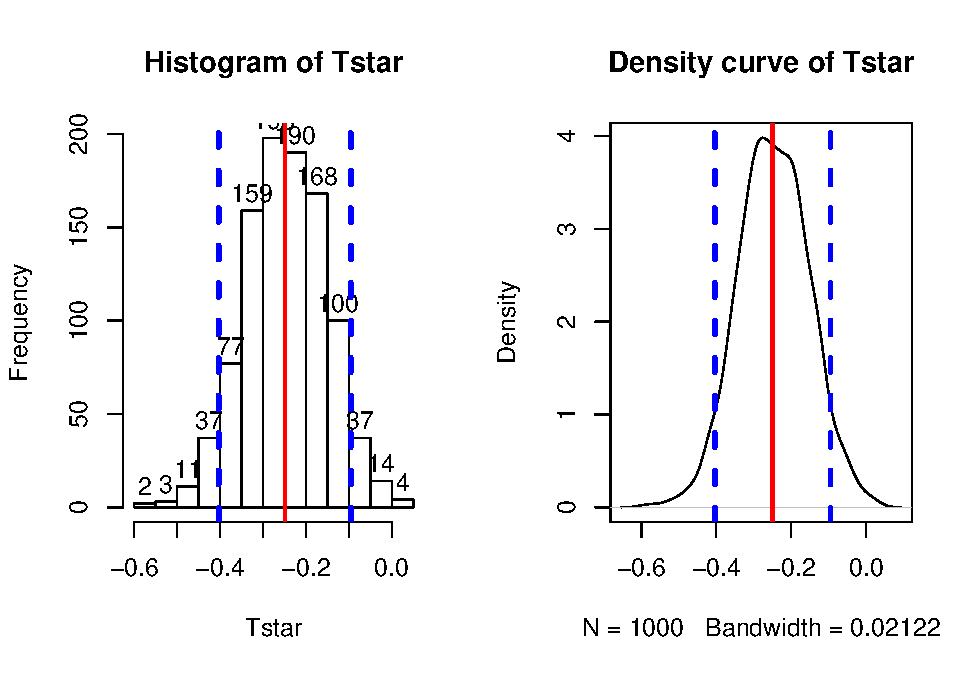
\includegraphics{GreenwoodBanner_files/figure-latex/Figure2-21-1.pdf}
\caption{\label{fig:Figure2-21}Histogram and density curve of bootstrap distribution of
difference in sample mean GPAs (male minus female) with observed
difference (solid vertical line) and quantiles that delineate the 90\%
confidence intervals (dashed vertical lines).}
\end{figure}

In the previous output, the parametric 90\% confidence interval is from
0.095 to 0.404, suggesting similar results again from the two approaches
once you account for the two different orders of differencing of the
groups. Based on the bootstrap CI, we can say that we are 90\% confident
that the difference in the true mean GPAs for STAT 217 students is
between -0.393 to -0.094 GPA points (male minus females). Because sex
cannot be assigned to the subjects, we cannot infer that sex is causing
this difference and because this was a voluntary response sample of STAT
217 students in a given semester, we cannot infer that a difference of
this size would apply to all STAT 217 students or even students in
another semester.

Throughout the semester, pay attention to the distinctions between
parameters and statistics, focusing on the differences between estimates
based on the sample and inferences for the population of interest in the
form of the parameters of interest. Remember that statistics are
summaries of the sample information and parameters are characteristics
of populations (which we rarely know). And that our inferences are
limited to the population that we randomly sampled from, if we randomly
sampled.

\section{Chapter summary}\label{section2-10}

In this chapter, we reviewed basic statistical inference methods in the
context of a two-sample mean problem. You were introduced to using R to
do permutation testing and generate bootstrap confidence intervals as
well as obtaining parametric \(t\)-test and confidence intervals in this
same situation. You should have learned how to use a \texttt{for} loop
for doing the nonparametric inferences and the \texttt{t.\ test}
function for generating parametric inferences. In the two examples
considered, the parametric and nonparametric methods provided similar
results, suggesting that the assumptions were at least close to being
met for the parametric procedures. When parametric and nonparametric
approaches disagree, the nonparametric methods are likely to be more
trustworthy since they have less restrictive assumptions but can still
have problems.

When the noted conditions are not met in a hypothesis testing situation,
the Type I error rates can be inflated, meaning that we reject the null
hypothesis more often than we have allowed to occur by chance.
Specifically, we could have a situation where our assumed 5\%
significance level test might actually reject the null when it is true
20\% of the time. If this is occurring, we call a procedure
\textbf{\emph{liberal}} (it rejects too easily) and if the procedure is
liberal, how could we trust a small p-value to be a ``real'' result and
not just an artifact of violating the assumptions of the procedure?
Likewise, for confidence intervals we hope that our 95\% confidence
level procedure, when repeated, will contain the true parameter 95\% of
the time. If our assumptions are violated, we might actually have an
80\% confidence level procedure and it makes it hard to trust the
reported results for our observed data set. Statistical inference relies
on a belief in the methods underlying our inferences. If we don't trust
our assumptions, we shouldn't trust the conclusions to perform the way
we want them to. As sample sizes increase and/or violations of
conditions lessen, then the procedures will perform better. In Chapter
\ref{chapter3}, we'll learn some new tools for doing diagnostics to help
us assess how much those conditions are violated.

\section{Summary of important R code}\label{section2-11}

The main components of R code used in this chapter follow with
components to modify in red, remembering that any R packages mentioned
need to be installed and loaded for this code to have a chance of
working:

\begin{itemize}
\item
  \texttt{summary}(\(\textcolor{red}{DATASETNAME}\))
\item
  \texttt{summary}({\texttt{DATASETNAME}})
\end{itemize}

\section{Practice problems}\label{section2-12}

\bibliography{packages,book}


\end{document}
